\documentclass[10pt]{report}

% Packages
\usepackage[dutch]{babel}
\usepackage[utf8]{inputenc}
\usepackage{datetime}
\usepackage[nottoc,numbib]{tocbibind}
\usepackage[table]{xcolor}% http://ctan.org/pkg/xcolor
\usepackage{graphicx}
\usepackage{caption}
\usepackage{fancyhdr}
\usepackage{wrapfig}
\usepackage{enumitem}
\usepackage{float}
\usepackage{afterpage}
\usepackage{dirtree}% https://ctan.org/pkg/dirtree
\usepackage[a4paper, margin=2cm]{geometry} % Margin eis: gemiddeld 2cm, breder mag, smaller niet.
\usepackage{booktabs}% http://ctan.org/pkg/booktabs
\usepackage{footnote}
\usepackage{bookmark}
\usepackage[toc,page]{appendix}
\usepackage{listings}
\usepackage{mathtools}
\usepackage{color}
\usepackage{hyperref}

% Configurations
\graphicspath{{assets/images/}}
\makesavenoteenv{tabular}
\makesavenoteenv{table}
\definecolor{background}{HTML}{EEEEEE}
% \colorlet{numb}{magenta!60!black}
\colorlet{numb}{white!60!black}

% XML listings
\definecolor{gray}{rgb}{0.4,0.4,0.4}
% \definecolor{darkblue}{rgb}{0.0,0.0,0.6}
% \definecolor{cyan}{rgb}{0.0,0.6,0.6}

\lstset{
  basicstyle=\ttfamily,
  columns=fullflexible,
  showstringspaces=false,
  commentstyle=\color{gray}\upshape
}

\lstdefinelanguage{XML}
{
  morestring=[b]",
  morestring=[s]{>}{<},
  morecomment=[s]{<?}{?>},
  stringstyle=\color{black},
  identifierstyle=\color{black},
  keywordstyle=\color{gray},
  morekeywords={xmlns,version,type}% list your attributes here,
  basicstyle=\normalfont\ttfamily,
  numbers=left,
  numberstyle=\scriptsize,
  stepnumber=1,
  numbersep=8pt,
  showstringspaces=false,
  breaklines=true,
  frame=lines,
  backgroundcolor=\color{background},
  literate=
     *{0}{{{\color{numb}0}}}{1}
      {1}{{{\color{numb}1}}}{1}
      {2}{{{\color{numb}2}}}{1}
      {3}{{{\color{numb}3}}}{1}
      {4}{{{\color{numb}4}}}{1}
      {5}{{{\color{numb}5}}}{1}
      {6}{{{\color{numb}6}}}{1}
      {7}{{{\color{numb}7}}}{1}
      {8}{{{\color{numb}8}}}{1}
      {9}{{{\color{numb}9}}}{1}
}

% JSON listings
\colorlet{punct}{black}
\definecolor{delim}{rgb}{0,0,0}
% \definecolor{delim}{RGB}{white!60!black}

\lstdefinelanguage{JSON}{
    basicstyle=\normalfont\ttfamily,
    numbers=left,
    numberstyle=\scriptsize,
    stepnumber=1,
    numbersep=8pt,
    showstringspaces=false,
    breaklines=true,
    frame=lines,
    backgroundcolor=\color{background},
    literate=
     *{0}{{{\color{numb}0}}}{1}
      {1}{{{\color{numb}1}}}{1}
      {2}{{{\color{numb}2}}}{1}
      {3}{{{\color{numb}3}}}{1}
      {4}{{{\color{numb}4}}}{1}
      {5}{{{\color{numb}5}}}{1}
      {6}{{{\color{numb}6}}}{1}
      {7}{{{\color{numb}7}}}{1}
      {8}{{{\color{numb}8}}}{1}
      {9}{{{\color{numb}9}}}{1}
      {:}{{{\color{punct}{:}}}}{1}
      {,}{{{\color{punct}{,}}}}{1}
      {\{}{{{\color{delim}{\{}}}}{1}
      {\}}{{{\color{delim}{\}}}}}{1}
      {[}{{{\color{delim}{[}}}}{1}
      {]}{{{\color{delim}{]}}}}{1},
}

% JavaScript listings
\lstdefinelanguage{JavaScript}{
  basicstyle=\normalfont\ttfamily,
  numbers=left,
  numberstyle=\scriptsize,
  stepnumber=1,
  numbersep=8pt,
  breaklines=true,
  frame=lines,
  backgroundcolor=\color{background},
  keywords={typeof, new, true, false, catch, function, return, null, catch, switch, var, if, in, while, do, else, case, break, constructor, instanceof, boolean, string, number},
  keywordstyle=\color{darkgray}\bfseries,
  ndkeywords={class, export, boolean, throw, implements, import, this},
  ndkeywordstyle=\color{darkgray}\bfseries,
  identifierstyle=\color{black},
  sensitive=false,
  comment=[l]{//},
  morecomment=[s]{/*}{*/},
  commentstyle=\color{black}\ttfamily,
  stringstyle=\color{gray}\ttfamily,
  morestring=[b]',
  morestring=[b]"
}

% Functionality
\newcommand{\tabitem}{~~\llap{\textbullet}~~}
\newcommand\blankpage{%
    \null
    \thispagestyle{empty}%
    \addtocounter{page}{-1}%
    \newpage}

% Literals
\newcommand{\versionnumber}{0.1}

\newcommand{\name}{Swen Meeuwes}
\newcommand{\studentnumber}{0887127}
\newcommand{\email}{0887127@hr.nl}
\newcommand{\mobilephone}{06 10 466 433}

\newcommand{\institution}{Hogeschool Rotterdam} %Rotterdam University of Applied Sciences
\newcommand{\organisation}{\&ranj}

\renewcommand{\title}{Een flexibele tool voor het vertellen van diverse digitale interactieve verhalen}
\newcommand{\subtitle}{}

% Lay-out
\renewcommand{\baselinestretch}{1.2} % Regelafstand eisen: minimaal 1.2; maximaal 1.5 regel
\pagestyle{fancy}
\fancyhf{}
\lhead{\leftmark}
\rhead{\name{}}
\lfoot{\title{}}
\rfoot{\thepage}


% Definitions
% hyperref
\def\figureautorefname{figuur}
\def\tableautorefname{tabel}
\def\appendixautorefname{bijlage}
\def\chapterautorefname{hoofdstuk}
\def\sectionautorefname{paragraaf}
\def\subsectionautorefname{alinea}

\begin{document}

\pagenumbering{roman}

\thispagestyle{empty}

\vspace*{4\baselineskip}

\begin{center}
    \Huge\title\\
    \Large\subtitle
\end{center}

\vspace{4\baselineskip}

\begin{center}
    \large
    {\name{}; \email}
\end{center}

\vspace{1\baselineskip}

\vfill


\vspace{1\baselineskip}

Studentennummer: \studentnumber{}\hfill\par
Datum: \today \hfill \par
Versie: \versionnumber{}\hfill
\afterpage{\blankpage}

\begin{titlepage}
    \begin{center}
      \Huge\title\\
      \Large\subtitle
    \end{center}

    \vspace{4\baselineskip}

    \Large \noindent
    {Auteur: \name{}; \email}\\
    {Bedrijf: \organisation{}}

    \vspace{1\baselineskip}

    \noindent
    {Bedrijfsbegeleider: I. Swartjes; ivo@ranj.nl}\\
    {1ste docent: I.S. Paraschiv; i.s.paraschiv@hr.nl}\\
    {2de docent: J. Grobben; j.grobben@hr.nl}\\

    % {Afstudeerscriptie voor ...}

    \vfill

    \begin{center}
      
\includegraphics[width=3cm]{University}

      \vspace{1\baselineskip}

      \Large
      CMI - Informatica\\
      \institution{}\\
      Nederland\\
      \today\\

      \vspace{1\baselineskip}

      \hfill Versie: \versionnumber\par
    \end{center}
\end{titlepage}

\afterpage{\blankpage}

\chapter*{Voorwoord}
Dit onderzoek is uitgevoerd en gedocumenteerd om de studie 'Informatica' aan de Hogeschool Rotterdam af te ronden. Hiervoor moet dit afstudeerverslag aantonen dat de student over de 4 competenties (Beheren, Analyseren, Adviseren, Ontwerpen) beschikt. Competenties en de lokaties waar zij worden aangetoond zijn opgenomen in de competentiewijzer (\autoref{app:competentiewzijer}).

\vspace{5mm}

\noindent
Allereerst wil ik mijn begeleiders, I. Swartjes en I.S. Paraschiv, bedanken voor de geweldige begeleiding die zij mij tijdens mijn afstudeerperiode hebben geboden. Wat heb ik het getroffen met jullie!

\vspace{5mm}

\noindent
Daarnaast wil ik \&ranj bedanken voor het aanbieden van een geweldige stageplek. Tijdens mijn afstudeerperiode was ik omringt door aardige en leuke collega's.

\vspace{5mm}

\noindent
Tenslotte wil ik Sofie, Elzeline, Gert-Jan, Anne en medestudenten Julian, Jesse, Corné bedanken voor alle feedback die zij mij hebben gegeven. In bijzonder wil ik Sofie, Elzeline en Gert-Jan bedanken voor alle steun die zij mij hebben geboden tijdens het afstuderen.
\afterpage{\blankpage}

\chapter*{Samenvatting}
In ontwikkelingsprocessen wordt er veel gebruik gemaakt van tooling om efficiëntie te verhogen. Dit onderzoek focust zich op tooling rondom het specificeren van content in het ontwikkelproces van narrative games. Deze tooling laat mensen zonder programmeerkennis content specificeren die later in de game getoond zal worden. Door een visual scripting interface aan te bieden kunnen gebruikers nodes met elkaar te verbinden om zo content te definiëren voor het narratief.
Tooling wordt over het algemeen geacht flexibel te zijn, zodat deze inzetbaar is in meerdere situaties.
\begin{quote} 
    \centering
    \large
    \textit{
        "Hoe kan er een flexibele tool worden opgezet voor het vertellen van diverse digitale interactieve verhalen?"
    }
\end{quote}

\noindent In dit onderzoek worden er stappen gezet richting een flexibelere tool voor het specificeren van content achter digitale interactieve verhalen. Typen content worden dynamische gedefinieerd, zodat de tool afgestemd kan worden op het project. Door in de tooling bij nodes en de structuur de scheiding te leggen tussen interpretatie en representatie kan er worden gewerkt met formalismen (e.g. story graphs, interactive behaviour trees) die aansluiten bij het project. In een overkoepelende projectstructuur komen overkoepelende constructen, zoals gedeelde variabelen, en de dynamische game content samen. Er is een prototype opgezet om deze concepten te ondersteunen en valideren.
%
% Het prototype is gebouwd met behulp van Electron, een ontwikkelplatform dat het gebruik van webtechnologieën voor het ontwikkelen van desktopapplicaties mogelijk maakt. Om de user interface synchroon te houden met de staat van de applicaties wordt er gebruik gemaakt van de React library. Tenslotte gebruikt het prototype de JointJS library om een visual scripting interface aan te bieden, zodat mensen zonder programmeerkennis de tool kunnen gebruiken.

Door middel van ‘content typen’ maakt het prototype onderscheid tussen verschillende soorten content. Dit zijn kleine datastructuren met een betekenis in de game. Door op een slimme manier gebruik te maken van JSON-schema kunnen deze content typen dynamisch worden gespecificeerd zonder de tool opnieuw te hoeven compileren. Dit maakt de tool flexibel en inzetbaar voor narrative games op een breed spectrum aan soorten content.

Het prototype legt een scheiding tussen formalisme en visuele componenten door gebruik te maken van het visitor design pattern. Het visitor pattern biedt context voor het transcompileren van visuele structuur naar dataformaat. Componenten worden gescheiden van hun representatie door het builder design pattern. Daarmee ondersteund de tool meerdere formalismen, zoals story graphs en interactive behaviour trees. Welke ieder gebruikt kunnen worden in een passende situatie. Dit maakt het onderhouden van meerdere tools met ieder zijn eigen formalisme overbodig en bevordert de flexibiliteit van de tool.

Wanneer er twee applicaties worden gebruikt voor het definiëren van het narratief (e.g. één voor het verhaal en één voor de dialoog) is het niet mogelijk om gedeelde variabelen in zowel verhaal als dialoog te gebruiken. Daarnaast weten deze applicaties niks af van bestanden (afbeeldingen, video's, geluiden) die in het narratief verworven worden. Naast dat het refereren naar deze bestanden foutgevoelig is, kunnen er geen previews van deze bestanden worden getoond in de tools. In een overkoepelende projectstructuur beheert de tooling haar bruikbare bestanden en kunnen overkoepelende constructen zoals gedeelde variabelen en content typen schema's ingericht worden per project.

% De tooling voor narrative games heeft te maken met vele bestanden (afbeeldingen, video’s, geluiden) die gebruikt worden in het narratief. Vooral grotere narrative games zijn gesplitst in bestanden die naast het verhaal ook dialogen bevatten. Deze bestanden die samen de game content vormen worden ook wel assets genoemd. Verder maken narrative games gebruik van variabelen om conditionaliteit af te dwingen. In dit onderzoek worden er stappen gemaakt richting een overkoepelende projectstructuur waarin game content geordend en met elkaar verbonden wordt. Zo kunnen overkoepelende variabelen gebruikt worden in zowel het verhaal als dialoog. Indien mogelijk kunnen assets worden gepreviewed in de editor. Hiernaast kunnen bestanden worden verplaatst binnen de assetsfolder zonder dat referenties gebroken worden. Tenslotte kunnen project specifieke configuraties worden opgenomen in de overkoepelende projectstructuur. Dit maakt het inrichten van content typen mogelijk per project.

Door slim gebruik te maken van JSON-schema’s voor het specificeren van content typen, een scheiding leggen tussen de editor en formalisme en het implementeren van een overkoepelende projectstructuur dienen allen als stap richting een flexibelere tool voor het vertellen van diverse digitale interactieve verhalen.

Dit onderzoek is uitgevoerd bij \&ranj, een serious game bedrijf dat zich specialiseert in narrative games. Met het maken van keuzes over ontwikkelplatformen wordt de huidige technology stack van \&ranj in kaart gebracht om te kijken of de keuze goed aansluit. Verder kan naast andere storytelling tools ook \&ranj gebruik maken van deze implementaties om hun tooling flexibeler te maken.

\chapter*{Management Summary}


\tableofcontents

\afterpage{
  \pagenumbering{arabic}
}

\chapter{Introductie}
\label{ch:introdcution}

\section{Achtergrond en aanleiding}
Rond 2008 begon \&ranj narratieven te verwerken in serious games om op verhalende wijze positieve gedragsverandering, zoals gezonder leven, toe te passen. Door gebruik te maken van de standaardisatie wist het bedrijf op een efficiënte manier meer dan 400 narrative game oplossingen te realiseren op klant specifieke problemen.

De narrative games van \&ranj dienen als een simulatie; een veilige omgeving waarin vooral soft skills beoefend kunnen worden. Soft skills zijn leiderschap, probleemgerichtheid en communicatieve vaardigheden. In het werkveld is er steeds meer vraag naar deze skills\cite{Gibert2017}\cite{Hirsch2017}\cite{Robles2012}. Echter zijn soft skills minder makkelijk te leren en te toetsen op scholen\cite{BishnuMurti2014}. Hiernaast kunnen dergelijke soft skills technische vaardigheden, ook wel hard skills genoemd, bevorderen\cite{Schulz2008}. Met deze games brengt \&ranj lastige onderwerpen ter tafel zoals peace building\footnote{https://ranj.com/projects/corporate/development\#missionzhobia} en discriminatie \footnote{https://ranj.com/projects/education\#fair-play}. Het doel van deze simulaties is dan ook om de speler bewust te maken van de gemaakte keuzes en positieve gedragsverandering te stimuleren.

\begin{wrapfigure}{r}{0.4\textwidth}
    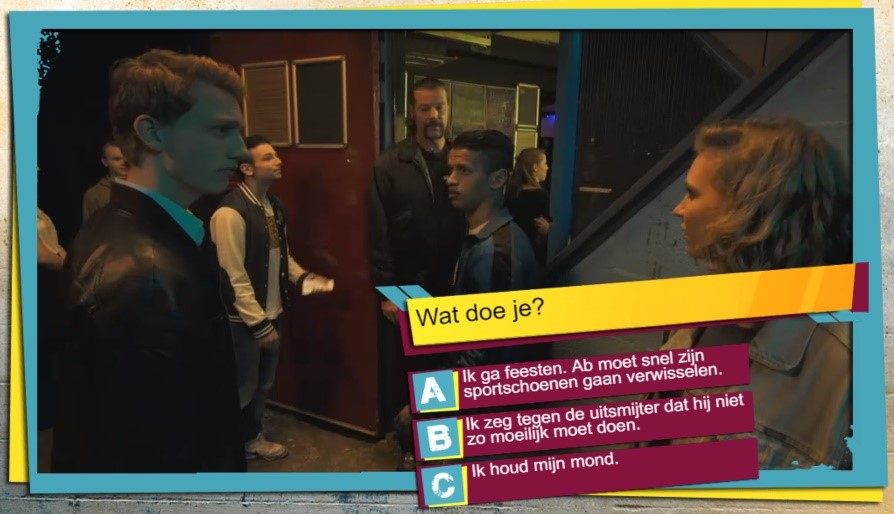
\includegraphics[width=0.38\textwidth]{FairPlayScreen}
    \caption{Een dialoog in de narrative game "Fair Play".}
    \label{fig:fairplayscreen}
    \centering
\end{wrapfigure}

Een narrative game bestaat uit een verhaallijn waarin de speler gesprekken voert met virtuele karakters om het verhaal te vorderen. Dit is goed terug te zien in de game “FairPlay” (\autoref{fig:fairplayscreen}). De games van \&ranj maken gebruik van fotografie, tekst en eventuele video en voice-overs om de speler in het verhaal te plaatsen (\autoref{fig:fairplayscreen}). Deze assets noemen we ook wel game content. Keuzes die de speler maakt hebben invloed op de loop en uitkomst van het verhaal. De speler krijgt directe feedback op zijn of haar gemaakte keuzes. Zo reflecteert het spel op eerder gemaakte keuzes in de vorm van een dialoog of report.

Met nieuwe hedendaagse technologieën wilt \&ranj haar narrative games naar het volgende niveau tillen. Deze toekomstblik noemen ze ‘narrative 2.0’ en staat op de roadmap van \&ranj. Als use case voor narrative 2.0 beschrijft het bedrijf een ‘bad news’ dialoog; een gesprek waarbij de speler slecht nieuws moet brengen. Een voorbeeld van een bad news gesprek is een ‘negatieve’ diagnose die als dokter gegeven moet worden. Deze dialogen willen ze zo realistisch mogelijk maken; succes hangt af van timing en gevoel. Realisme in games wil het bedrijf bereiken door onder andere artificial intelligence (AI) oplossingen toe te passen.

\pagebreak
Om narrative 2.0 te ondersteunen is er vraag naar tooling, externe hulpprogramma(s) die productiviteit bevorderen\cite{Pizzi}, die zal helpen bij het ontwikkelproces van de toekomstige narrative games. Het bedrijf beschikt over twee applicaties waarin narratieven geschreven kunnen worden zonder enige programmeerkennis. Deze applicaties heten de story- en dialog editor. In deze bewerkers kunnen verhalen worden gemoduleerd. Ze bestaan uit een interface waarin content types in nodes worden gerepresenteerd. Een content type is een datastructuur met een betekenis in de game. Het content type ‘ImageContent’ zou bijvoorbeeld als doel hebben om een afbeelding tonen. Tenslotte verbinden edges de content met elkaar (\autoref{fig:visualscriptingineditor}).

Deze story- en dialog editor heeft het bedrijf in 2008 opgezet met behulp van de Apache Flex SDK en ActionScript3. Over de jaren heen zijn de verwachtingen van de bewerkers veranderd, maar ze zijn niet uitgebreid omdat de achterliggende softwarearchitectuur niet houdbaar en flexibel is. Dit zorgt voor problemen bij het ontwikkelproces van zowel huidige als toekomstige narrative games zoals de ‘bad news’ game. \&ranj wilt inzicht krijgen in wat er nodig is om een nieuwe editor op te zetten die oplossingen biedt op de huidige problemen.

\begin{figure}[htb]
    \centering
    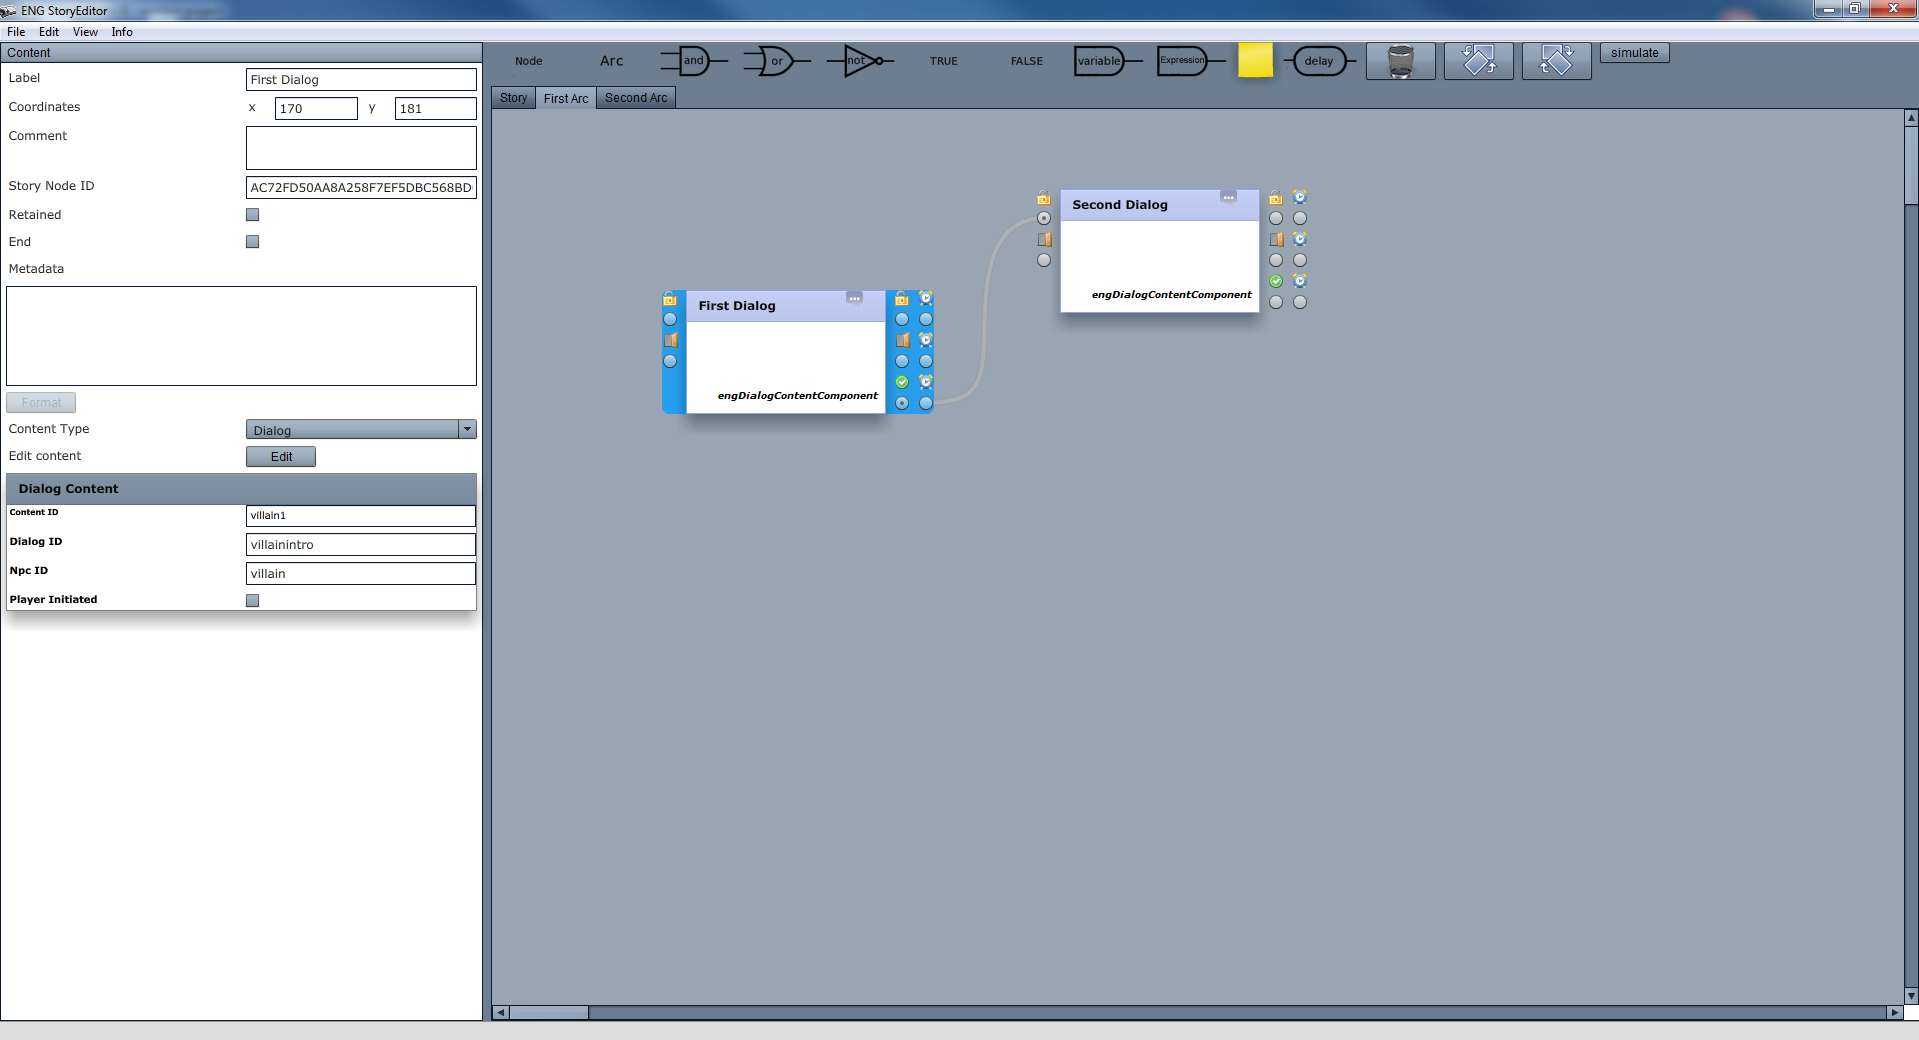
\includegraphics[width=0.92\textwidth]{VisualScriptingInEditor}
    \caption{Visual scripting in de Story Editor.}
    \label{fig:visualscriptingineditor}
\end{figure}

\pagebreak
\section{Probleemstelling}
De story- en dialog editor zijn opgezet om medewerkers zonder programmeerkennis game content zelfstandig te laten bewerken. Deze tooling wordt gebruikt in alle narrative game projecten en is essentieel voor het ontwikkelproces en productiviteit. Hiernaast bevordert het itereren over game content en maakt deze inzichtelijk door de game content te visualiseren. Hierbij speelt flexibiliteit een grote rol. De editors moeten flexibel genoeg zijn om bruikbaar te zijn voor verschillende narrative game projecten.

Het bedrijf werkt toe naar nieuwe tooling en wilt inzicht verkrijgen in het opzetten van flexibele oplossingen. Dit leidt dan ook tot de centrale onderzoeksvraag: 

\begin{quote} 
    \centering
    \large
    \textit{
        "Hoe kan er een flexibele tool worden opgezet voor het vertellen van diverse digitale interactieve verhalen?"
    }
\end{quote}

\subsection{De technology stack}
Het huidige gebruikte platform, Apache Flex, heeft weinig libraries die gebruikt kunnen worden voor de interface van de editors. Libraries zijn collecties aan code en configuraties die gebruikt kunnen worden in andere applicaties. Meestal richten ze zich op een veelvoorkomend probleem, zodat programmeurs niet telkens het wiel opnieuw uit hoeven te vinden. De libraries die beschikbaar zijn voor Apache Flex, zoals ‘Flex Wires’ die de verbindingen tussen nodes mogelijk maakt, hebben weinig functionaliteit en bevatten bugs. \&ranj wilt naar een platform met een grotere community en meer flexibiliteit in frameworks en libraries, zodat het wiel niet telkens opnieuw uitgevonden hoeft te worden.

Hiernaast is het ultieme einddoel om een webapplicatie te maken waarin meerdere personen tegelijk aan een narratief kunnen werken. Collaborative editing, het ondersteunen van aanpassingen door meerdere personen tegelijk, kan het makkelijker maken om samen met klanten te werken.

\subsection{Diversiteit in game content}
Uit eerdere projecten die verschillen in game content blijkt dat de huidige editors niet flexibel genoeg zijn. Het probleem ligt vooral aan de diversiteit in game content tussen projecten. Echter is dit wel een eis sinds \&ranj voor verschillende klanten werkt waarvan ieder een eigen beroepenveld heeft. Dit dwingt diversiteit in game content af.

In de game content speelt semantiek een grote rol. De interpretatie van een content type hangt af van haar semantische eigenschappen. In de huidige editors hebben content types een statische definitie. Om nieuwe content types toe te voegen moeten de content types gedefinieerd worden in de broncode; content types zijn hard gebakken in de editors. Het opzetten, uitbreiden, compileren en deployen van de editors is een langdurig proces dat met de hand uitgevoerd moet worden. Voor ieder project moeten er nieuwe editors met de benodigde content types worden gebouwd. Hierbij moet er ook nog eens op gelet worden dat oudere content types functioneel blijven, zodat de editors de data van oudere narrative games nog kunnen uitlezen. Dit maakt het erg lastig om de huidige story- en dialog editor in te zetten voor verschillende projecten vanwege de tijd en dus geld die het kost om content types toe te voegen. Vaak wordt dit ondanks de kosten wel gedaan wat resulteert in een uitbreidende selectie aan content types. Echter zijn deze content types meestal zo project specifiek dat ze niet in meer dan één project gebruikt worden. Dit resulteert in een onoverzichtelijke editor, omdat de niet gebruikte content types wel in de editor zitten.

\pagebreak
\subsection{Het ondersteunen van meerdere formalismen}
In de huidige editors bestaat er een nauwe koppeling tussen de visual scripting interface en het achterliggende formalisme. Dit maakt het lastig om van formalisme te veranderen, laat staan nieuwe formalisme te ondersteunen. Deze beperking verlaagd de flexibiliteit en inzetbaarheid van de editors. In de roadmap van het bedrijf wordt beschreven hoe \&ranj een ‘smart follower’ wilt zijn onder andere op het gebied van artificial intelligence (AI). Er gebeurt erg veel op het gebied van AI en \&ranj ziet mogelijkheden om deze nieuwe technologie toe te passen in toekomstige games. Door op de hoogte te blijven van AI kan het bedrijf nieuwe aantrekkelijke oplossingen verwerken in hun games en deze verkopen aan de klant. Met de huidige story- en dialog editor is het vrijwel onmogelijk om gebruik te maken van AI. Het achterliggende formalisme biedt alleen de mogelijkheid om content types aan elkaar te verbinden en zo een graph te vormen. Om AI toe te passen in narrative games moet er gebruik gemaakt worden van formalismen die dit ondersteunen. In tegenstelling tot het huidige formalisme waarin opeenvolgende instructies gedefinieerd worden bieden behaviour trees een meer AI georiënteerde oplossing\cite{Pizzi}\cite{Lim2010}.

\subsection{Overkoepelende projectstructuur}
Hoewel de dialog- en story editor het narratief ordent en aan elkaar verbindt beheert zij de bijbehorende game content niet; er is geen sprake van een overkoepelde projectstructuur. Een voorbeeld hiervan is hoe de huidige editors om gaan assets, bestanden die gebruikt worden in de game. Er moet handmatig een manifest worden bijgehouden waarin assets een sleutel (id) en semantiek toegekend krijgen (zie \autoref{fig:gamecontentmanifest}). Deze sleutel wordt gebruikt in de huidige editors om te kunnen refereren naar assets, zoals geluid, afbeeldingen en videos. Zo refereert het content type ‘image content’ naar een asset via een sleutel. Deze asset zou een afbeelding moeten zijn, maar er bestaat geen zekerheid over dat de asset een afbeelding is of überhaubt bestaat. Dit zorgt voor een zwakke link tussen de editors en game content, wat het erg gevoelig maakt voor (menselijke)fouten. Zo hoeft er maar één typefout gemaakt of het pad aangepast te worden om de referentie naar de game content te verliezen.

\begin{figure}[htb]
    \centering
    \lstset{language=JSON}
    \begin{lstlisting}
    {
        "scenario_test": [{
            "id": "story_scenario_test",
            "type": "json",
            "src": "assets/scenarios/scenario_test/story.json"
        }],
        "sounds": [{
            "id": "backgroundmusic",
            "type": "sound",
            "src": "assets/sounds/backgroundmusic.mp3"
        }]
    }
    \end{lstlisting}
    \caption{Game content manifest.}
    \label{fig:gamecontentmanifest}
\end{figure}

\pagebreak
\section{Doelstelling}
\subsection{Vanuit \&ranj}
Het bedrijf hoopt in 2019 nieuwe editor(s) op te zetten die het ontwikkelproces van narrative games zullen ondersteunen. Om de diversiteit in klanten en de toekomstplannen van de editors te ondersteunen moeten de nieuwe editor(s) flexibel opgezet zijn, zodat het op maat maken van de games mogelijk is. Zo moet de nieuwe editor kunnen omgaan met de diversiteit in game content, een deel uit maken van een overkoepelende projectstructuur en het achterliggende formalisme scheiden van de user interface.

\subsection{Uit persoonlijk interesse}
Een zelfstandig eigen project drie jaar terug was mijn eerst aanraking met het concept van een narrative game. Er was een duidelijke behoefte naar tooling om het verhaal in te schrijven. Het makkelijk kunnen aanpassen van het verhaal was een probleem, omdat er geen externe tooling voor bestond die goed aansloot bij de wensen van het project destijds. Hoewel het een erg leuk project was om naast mijn studie op te pakken, bracht het veel werk met zich mee waardoor het nooit gelukt is om het project af te ronden. Dit onderzoek kan inzicht bieden in hoe dit beter aangepakt had kunnen worden.

\subsection{Vanuit school}
Het onderzoek moet gedocumenteerd worden in de vorm van een scriptie. Deze scriptie moet voldoen aan de beoordelingscriteria die vooraf opgesteld zijn. Er moet tijdens het onderzoek voldaan worden aan 4 competenties: beheren, analyseren, adviseren en ontwerpen. Tenslotte moet er sprake zijn van een professionele houding en adequate communicatie met de stakeholders. De beoordeling volgt uit de scriptie en eindpresentatie.


\section{Onderzoeksvragen}
\subsection{Hoofdvraag}
Vanuit het probleem is de volgende centrale onderzoeksvraag opgesteld:
\begin{quote} 
    \centering
    \large
    \textit{
        "Hoe kan er een flexibele tool worden opgezet voor het vertellen van diverse digitale interactieve verhalen?"
    }
\end{quote}

\subsection{Deelvragen}
Om de centrale onderzoeksvraag te kunnen beantwoorden zijn de volgende deelvragen opgesteld:
\begin{itemize}
    \item Hoe kan er een ‘technology stack’ opgezet worden die een flexibele basis biedt voor een editor waarmee diverse digitale interactieve verhalen verteld kunnen worden?
    \item Hoe kan diverse game content ondersteund worden?
    \item Hoe kan de architectuur achter de editor zo worden opgezet dat er in latere stadia nieuwe narratieve formalismen makkelijk doorgevoerd kunnen worden?
    \item Hoe kan game content in de overkoepelende projectstructuur verbonden en geordend worden?
\end{itemize}

\pagebreak
\section{Scope}
Het onderzoek vindt plaats over een tijdsduur van 20 weken. Omdat er gewerkt wordt met een tijdslimiet is het belangrijk om een scope vast te leggen. Naast dat deze afbakening overzicht en focus biedt voorkomt deze misverstanden tussen de betrokken partijen.

\noindent Dit onderzoek omvangt:
\begin{itemize}
    \item Het doorspitten van de broncode achter de huidige editors.
    \item Eventuele prototypes om standpunten te onderbouwen.
    \item Advies op het gebied van ontwikkelplatformen, libraries en architectuur.
    \item Het in kaart brengen van de huidig gebruikte technologieën.
    \item Een scriptie schrijven met daarin adviezen en conclusies over het desbetreffende onderwerp.
\end{itemize}

\noindent Er zal geen aandacht besteed worden aan:
\begin{itemize}
    \item Het ontwikkelen van een productie klare editor die direct inzetbaar is voor toekomstige narrative game projecten.
    \item Een narrative game ontwikkelen met de eventuele gemaakte prototypes.
    \item Verdieping in klant co-creatie.
    \item Onderzoek naar ‘collaborative editing’.
    \item De deployment pipeline van de editors.
    \item Optimalisatie van de editors.
    \item Het dataformaat waarmee de editors communiceren met de game engine.
\end{itemize}

\pagebreak
\section{Structuur}
Deze paragraaf geeft inzicht in de komende hoofdstukken van de scriptie en dient als een kapstok voor de lezer. Zo wordt er bij ieder hoofdstuk beschreven wat de lezer kan verwachten.

\begin{description}
    \item[Hoofdstuk 2] omschrijft welke methodes er gebruikt zijn om tot de behaalde resultaten te komen.
    \item[Hoofdstuk 3] geeft context aan het onderzoek en plaats deze in een groter plaatje.
    \item[Hoofdstuk 4] betreft de onderliggende bouwblokken waarop de huidige applicatie gebouwd is en waarop de nieuwe applicatie gebouwd zal worden; de ‘technology stack‘. Het belang van een goedpassende tech stack komt ter sprake en er worden adviezen gedaan over benodigde veranderingen binnen de stack die aansluiten op het toekomstbeeld bij de editors.
    \item[Hoofdstuk 5] beschrijft hoe er onderscheid wordt gemaakt tussen game content. Hiernaast gaat dit hoofdstuk in op de diversiteit in game content en hoe deze ondersteund kan worden.  
    \item[Hoofdstuk 6] betreft de rol van formalisme binnen interactive story telling, de formalismen die gebruikt worden in de huidige editors en het leggen van een scheiding tussen de editors en achterliggende formalisme.
    \item[Hoofdstuk 7] gaat in op de behoefte aan een overkoepelende projectstructuur en eventuele stappen die gemaakt kunnen worden.
    \item[Hoofdstuk 8] beschrijft de eindconclusie van het onderzoek.
    \item[Hoofdstuk 9] geeft inzicht in de adviezen die voort zijn gekomen uit het onderzoek. Hiernaast komen ook eventuele aandachtspunten of vervolgonderzoek ter sprake.
    \item[Hoofdstuk 10] omvat een reflectie op de afstudeerstage het onderzoek.
    \item[Hoofdstuk 11] bevat een lijst met begrippen en verwijzingen naar waar het begrip staat uitgelegd.
\end{description}


\chapter{Bedrijf}
\label{ch:bedrijf}
Dit hoofdstuk biedt informatie over het bedrijf waarbij het onderzoek is uitgevoerd. Hiernaast geeft het inzicht in welke afdeling van het bedrijf het onderzoek gedaan is. 

\section{\&ranj}
\&ranj is een internationaal bedrijf dat sinds 1999 serious game oplossingen realiseert. Dit zijn spellen waarbij de speler spelenderwijs getraind wordt. Een voorbeeld hiervan is de serious game ‘Mission Zhobia – Winning the Peace’\footnote{\url{https://www.missionzhobia.org/}}. In deze game wordt de speler getraind in peace building. Het bedrijf heeft te maken met klanten in diverse vakgebieden. Hierdoor is het domein van de onderwerpen erg breed.

\&ranj wilt mensen helpen ontwikkelen op een effectieve en efficiënte manier. Met behulp van ‘serious games’ wilt het bedrijf voor de gebruiker een ervaring creëren waarin hij of zij kennis opdoet om in het echte leven uitdagingen aan te gaan en leert problemen te tackelen. Volgens \&ranj is de beste manier van leren het leren door te doen.

\section{Visie}
Met serious games past \&ranj op spelenderwijze gedragsverandering toe, om zo een betere toekomst te bouwen. De visies van \&ranj luiden:

\begin{quote} 
    \centering
    \large
    \textit{
        “Together we build a brighter future”
    }\\
    \&\\
    \textit{
        “We achieve positive behavioural change through play”
    }
\end{quote}

\section{Afdelingen}
\label{sec:afdelingen}
Het bedrijf specialiseert zich in drie verschillende richtingen met ieder zijn eigen specialiteit. Deze richtingen kunnen omschreven worden met verschillende keywords.
\begin{itemize}
    \item Gamification; gefocust op: “consultancy”, “leuk maken van minder leuke taken/ werk”, “fysiek”.
    \item Playground; gefocust op: “experimentatie” en “ervaringen”.
    \item Corporate Learning; gefocust op: “soft skills”, “volwassen organisaties”, “bewezen oplossingen” en “efficiëntie”.
\end{itemize}
Dit onderzoek vindt plaats in de 'corporate learning’ afdeling.

\section{Corporate learning}
\label{sec:corporatelearningafdeling}
De corporate learning afdeling van \&ranj realiseert oplossingen voor “volwassen” bedrijven die soft skills bij hun werknemers willen bevorderen. Bij deze afdeling ligt de nadruk op efficiëntie en het gebruikt van oplossingen waarvan het bedrijf weet dat ze werken. Meestal zijn deze oplossingen narrative games, spellen waarin op verhalende wijze kennis wordt overgebracht.

Het ontwikkelen van een narrative game is een grote compliceert proces. Dit onderzoek zal zich alleen focussen op de ontwikkelingsfase, omdat de editors daar een grote rol in spelen. In deze fase werkt het team samen om het product te realiseren.

\begin{wrapfigure}{r}{0.45\textwidth}
    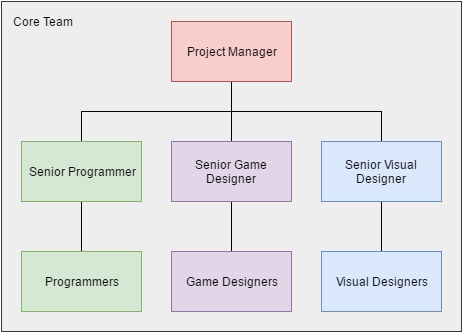
\includegraphics[width=0.43\textwidth]{CoreTeam}
    \caption{Anatomie van een core team bij \&ranj.}
    \label{fig:coreteam}
    \centering
\end{wrapfigure}

Een corporate learning development team bestaat uit de volgende disciplines:

\begin{description}
    \item[Programmeur] Is verantwoordelijk voor de technische implementatie van de game. Hiernaast biedt deze ondersteuning bij technische vraagstukken. 
    \item[Game designer] Is verantwoordelijk voor de mechanieken en het verhaal achter de game. Hij of zij probeert gedragsverandering toe te passen met de game als tool. Verder werken game designers nauw samen met de projectmanager om te zorgen dat de game aansluit bij de wensen van de klant.
    \item[Visual designer] Is verantwoordelijk voor de visuals binnen de game. Een visual designer wilt door middel van deze visuals meestal een gevoel bij de speler oproepen.
    \item[Projectmanager] Begeleid het ontwikkelproces en is regelmatig in contact met de klant. Hij of zij zorgt dat het project binnen het budget blijft en onderhandeld met de klant wanneer nodig. De projectmanager trekt aan de bel als het project niet aansluit bij de wensen van de klant en heeft veto op de keuzes binnen het project.    
\end{description}

\noindent Het kan zijn dat er meerdere programmeurs, game designers of visual designers aan een project werken. Als dit het geval is wordt er een senior als lead aangewezen. De lead begeleid de teamleden met dezelfde rol.

\pagebreak
\subsection{Ontwikkelproces van narrative games}
\label{subsec:ontwikkelprocesnarrativegames}
Het ontwikkelen van een narrative game kan een ingewikkeld proces zijn dat veel tijd kan kosten. Dit ligt aan de complexiteit van het verhaal en eventuele achterliggende modellen. In het verhaal kan de speler keuzes maken waarbij elke keuze meestal tot een ander pad in het verhaal leidt.

Dit maakt het onmogelijk om het verhaal te definiëren in code of een bestaand dataformaat. Tenslotte wordt het handmatig vast leggen van het verhaal in een dataformaat zoals JSON of XML al gauw onoverzichtelijk. Dit zorgt voor een probleem in het ontwikkelproces.

Om dit probleem te tackelen en het ontwikkelproces efficiënter te laten verlopen heeft het bedrijf in 2008 het ontwikkelproces van narrative games gestandaardiseerd. Onder efficiënt verstaan we in dit geval het versnellen van het proces en het voorkomen van fouten in de game. 

Ter ondersteuning en standaardisatie van het ontwikkelproces zijn de story- en dialog editor gebouwd. Deze editors laten game designers zonder enige programmeerkennis verhalen en dialogen schrijven.

Om de efficiëntie van het ontwikkelproces van een narrative game verder te verhogen heeft het bedrijf een template opgezet voor het ontwikkelen van narrative games. Dit template noemen ze het narrative game template (NGT) en dient als een geteste basis voor narrative games. Het NGT verwerkt geëxporteerde data uit de story- en dialog editor en is het deel dat uiteindelijk de verschillende content types toont/ evalueert. Een overzicht van de relaties tussen de editors en het NGT is terug te zien in \autoref{fig:ontwikkelomgevingnarrative}. 

\begin{figure}[htb]
    \centering
    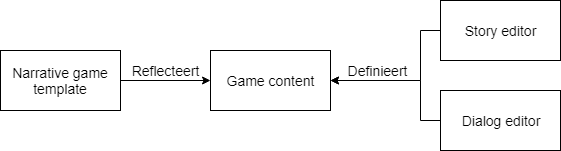
\includegraphics[width=0.7\textwidth]{OntwikkelOmgevingNarrative}
    \caption{Ontwikkelomgeving voor interactieve narratieve.}
    \label{fig:ontwikkelomgevingnarrative}
\end{figure}



\chapter{Methodiek}
\label{ch:methodes}
Dit hoofdstuk omschrijft de methodes en werkwijzen die toegepast zijn tijdens dit onderzoek om tot de behaalde resultaten te komen. Deze methodes en werkwijzen worden vervolgens gekoppeld aan toekomstige hoofdstukken en geven inzicht in hoe er te werk is gegaan.

\section{Onderzoeksmethodieken}
Tijdens het onderzoek is er gebruik gemaakt van verschillende onderzoekmethodieken om zowel kennis te vergaren als te valideren. In deze paragraaf worden de gebruikte onderzoeksmethodieken gelinkt aan de deelvragen waarvoor ze gebruikt zijn.

\subsection{Literatuuronderzoek}
Tijdens dit onderzoek is er gebruik gemaakt van literatuuronderzoek om informatie over het desbetreffende onderwerp te vergaren en eventuele oplossingen te valideren. Er is gebruik gemaakt van boeken, papers en wanneer deze schaars waren artikelen, blogs en fora. Hierbij is er goed gekeken naar de betrouwbaarheid van de bron. Bronnen zijn geëvalueerd op hun betrouwbaarheid door andere bronnen met hetzelfde of een overlappend onderwerp te vergelijken. Hiernaast is er gekeken naar objectiviteit van de schrijver, de datum van de bron en welke referenties gebruikt worden om argumenten te onderbouwen.

Hoewel dit onderzoek vrij niché is en er weinig bronnen bestaan over het onderwerp, wordt er literatuuronderzoek gebruikt waar dit nuttig en mogelijk is. Bij deelvragen 1, 2, 3 en 4 wordt er gebruik gemaakt van literatuuronderzoek.

\begin{itemize}
    \item De eerste deelvraag, \autoref{ch:technologystack}, maakt gebruik van literatuuronderzoek om de keuze achter de nieuwe technology stack te onderbouwen.
    \item De tweede deelvraag, \autoref{ch:diversiteitingamecontent}, maakt gebruik van literatuuronderzoek om kennis te vergaren over dataschema’s.
    \item De derde deelvraag, \autoref{ch:formalism}, maakt gebruik van literatuuronderzoek om design patterns en hun consequenties in kaart te brengen.
    \item De vierde deelvraag, \autoref{ch:overkoepelendeprojectstructuur}, maakt gebruik van literatuuronderzoek om te kijken hoe andere applicaties met een overkoepelende projectstructuur omgaan met bestanden.
\end{itemize}

\pagebreak
\subsection{Implementatie gedreven onderzoek}
Om eventuele oplossingen op architecturele vraagstukken te valideren is er gebruik gemaakt van implementatie gedreven onderzoek. Naast validatie geeft deze methode inzicht in eventuele consequenties en andere vraagstukken die opkomen. Dit is een van de sterkere vormen van validatie, omdat de oplossing gelijk in werking wordt gezet.

Aan deze onderzoeksmethode zitten wel 2 risico’s verbonden waarmee rekening gehouden moet worden\cite{ResearchSkillsInComputerScience}. Het vraagstuk moet (1) eerst duidelijk in kaart gebracht en vastgesteld worden. Als het vraagstuk veranderd, door eventuele nieuwe inzichten, is de validatie gehaald uit de implementatie niet meer geldig. Hiernaast is het (2) lastig om een generieke implementatie te gebruiker ter validatie, omdat de implementatie voor ieder system mogelijk zal verschillen.

Uit het ‘implementatie gedreven onderzoek’ zal een prototype komen die dient als ondersteuning en validatie van de onderzoeksresultaten en voorstellen. Dit prototype beschikt alleen over functionaliteiten waarvoor gebruik gemaakt is van deze onderzoeksmethode. Dit betekent dat het prototype \underline{\textbf{niet}} dient als een inzetbaar prototype, minimal viable product of basis voor het toekomstige product; het prototype is gebouwd op “weggooi code”.

Implementatie gedreven onderzoek is toegepast om deelvragen 1, 2 en 3 te valideren. Verder bracht deze methode vraagstukken naar boven die besproken zullen worden in de desbetreffende hoofdstukken.

\begin{itemize}
    \item De eerste deelvraag, \autoref{ch:technologystack}, maakt gebruik van implementatie gedreven onderzoek om het voorstel voor de nieuwe technology stack te valideren. Hierbij zullen de nieuwe technologieën gebruikt worden in het prototype en zo gevalideerd worden.
    \item De tweede deelvraag, \autoref{ch:diversiteitingamecontent}, maakt gebruik van implementatie gedreven onderzoek om de toepassing van JSON-schema’s te valideren. Het prototype zal gebruik maken van JSON-schema om diverse game content te ondersteunen.
    \item De derde deelvraag, \autoref{ch:formalism}, maakt gebruik van implementatie gedreven onderzoek om de architecturele keuze te valideren. Deze keuze betreft het omzetten van de visuele structuur naar een exportbestand, waarbij formalisme gescheiden wordt van de visuele representatie.
\end{itemize}
    
\subsection{Bureauonderzoek}
Tijdens dit onderzoek is er gebruik gemaakt van bureauonderzoek om informatie te vergaren over de populariteit en toekomst van bepaalde softwareoplossingen/ technologieën. Hiermee wordt de grootte en activiteit van community’s rondom technologieën ingeschat.

Bureauonderzoek wordt toegepast om informatie te vergaren in deelvragen 1 en 2.
\begin{itemize}
    \item De eerste deelvraag, \autoref{ch:technologystack}, maakt gebruik van bureauonderzoek om de populariteit en grootte van de community rondom ontwikkelplatformen in te schatten. Hiernaast wordt hetzelfde gedaan voor diagramming libraries en user interface libraries \& frameworks. 
    \item De tweede deelvraag, \autoref{ch:diversiteitingamecontent}, maakt gebruik van bureauonderzoek om de community rondom JSON-schema’s in te schatten. Er wordt gekeken of er bestaande oplossingen zijn betreft het manipuleren, valideren en reflecteren van JSON-schema’s die gebruikt kunnen worden voor de nieuwe editor.
\end{itemize}

\pagebreak
\section{Werkwijzen}
Tijdens dit onderzoek zijn er werkwijzen gedefinieerd die bijdragen aan het gewenste eindresultaat. In deze paragraaf wordt besproken hoe de verschillende werkwijzen toegepast zijn.

\subsection{Wekelijkse meetings}
Tijdens de stageperiode zijn er wekelijks meetings in gepland met de bedrijfsbegeleider die ook als opdrachtgever fungeerde. Deze meetings duurde rond een uur waarin de bedrijfsbegeleider op de hoogte werd gebracht. Hiernaast waren dit de momenten om een discussie aan te gaan over vraagstukken die op dat moment speelden.

Aan het begin van het onderzoek zijn deze meetings gebruikt om huidige problemen en vraagstukken in kaart te brengen. Hiernaast werd er een toekomstbeeld van de editors geschetst. Hieruit zijn de deelvragen geformuleerd en vervolgens gevalideerd met de bedrijfsbegeleider. Dit was noodzakelijk voor de scope en afbakening van het onderzoek.

Tijdens het ‘implementatie gedreven onderzoek’ diende de meetings als validatie. Hierbij werd de opgestelde hypothese onderbouwd met een prototype. Hiernaast werden bevindingen besproken en gevalideerd.

\subsection{Het doorspitten van broncode}
De vraag naar dit onderzoek kwam voort uit het gebruiken van de huidige editors. Om een beter beeld te krijgen van wat het probleem echt inhoud is er gekeken naar de broncode van de editors. Zo kon de huidige technology stack en de problemen die deze met zich meebracht in kaart worden gebracht. Ook werd het duidelijk waarom de grote diversiteit aan game content een probleem is in de huidige editor. Tenslotte kon er inzicht vergaard worden in verschillende formalisme achter de editors en hun nauwe koppeling met de visual scripting interface.

\subsection{Meewerken aan een narrative project}
Voorafgaand aan het afstudeertraject is er een jaar lang meegewerkt aan narrative game projecten. Tijdens deze projecten is er veel ervaring opgedaan met de story- en dialog editor en hun achterliggende concepten. Deze ervaring is erg waardevol voor dit onderzoek, omdat het inzicht gaf in de huidige stand van zaken. Hiernaast biedt het oplossen van veel voorkomende problemen met deze editors extra motivatie om het onderzoek af te nemen en te voltooien.

Naast deze positieve kant introduceert het ook een groot risico. Tijdens het onderzoek moest er goed op worden gelet dat er geen aannames gedaan werden en dat er niet vanuit eigen ervaring gekeken werd. Om dit tegen te gaan zijn er wekelijkse meetings ingepland met de opdrachtgever. Deze heeft een goed beeld van de huidige situatie en problemen die hierin spelen. Hij werkt samen met andere programmeurs en game designers die gebruik maken van de editors en bespreekt voorkomende problemen met de gebruikers.

\subsection{Versiebeheer}
Tijdens het onderzoek is er gebruik gemaakt van versiebeheer. Door gebruik te maken van GitHub waren de scriptie en het prototype overal en voor iedereen beschikbaar. Hierdoor kon het onderzoek uitgevoerd worden op meerdere computers en was het prototype makkelijk in te zien. Hiernaast biedt GitHub meer zekerheid dan een individuele computer op het gebied van data persistentie; als de computer crasht en alle data verloren gaat is het onderzoek niet verloren.

Voor het prototype was het van belang om eventueel terug te kunnen rollen naar een eerder werkende versie. Hiernaast kon er altijd een aftakking worden gemaakt waarin een feature geïmplementeerd kon worden zonder de werkende versie te breken.

Zowel de scriptie\footnote{https://github.com/swenmeeuwes/thesis} als het prototype\footnote{https://github.com/swenmeeuwes/concept-narrative-editor-framework} zijn beschikbaar op GitHub.



\chapter{Technologieën}
\label{ch:technologystack}
In dit hoofdstuk wordt er gekeken naar technologieën die eventueel toepasbaar zijn op het ontwikkelproces van de nieuwe editor. Eerst zullen de huidige gebruikte technologieën op een rijtje worden gezet. Hierna zal er gekeken worden naar de toekomst van de editors. Tenslotte zal het probleem in kaart worden gebracht waarop eventuele oplossingen zullen worden geadviseerd.

\section{Technology stack}
Onder een ‘technology stack’ (of ‘tech stack’) verstaan we de onderliggende bouwblokken waarop de desbetreffende applicatie gebouwd is. Deze bouwblokken bestaan uit onder andere frameworks, libraries, programmeertalen, softwareproducten en eventuele tooling\cite{BlogTechStack}.

\subsection{Waarom is dit belangrijk?}
Het is erg belangrijk om de tech stack in kaart te brengen omdat er elementaire informatie uit te halen is. De tech stack geeft inzicht in hoe het huidige product in elkaar steekt en eventuele consequenties wanneer er componenten in de stack aangepast worden. Dit is noodzakelijk voor het maken van een nieuwe editor die geïntegreerd moeten worden in een al bestaande tech stack. Door deze stap te nemen wordt er goed gekeken naar hoe de nieuwe editor in het totaal plaatje zou kunnen passen. Zo kan het voor komen dat er bepaalde software wordt gebruikt die nauw samenwerkt met de huidige editors. Dit heeft als gevolg dat de nieuwe editors deze samenwerking moeten ondersteunen.

\pagebreak
\section{De technology stack van \&ranj}
Om de ontwikkeling van narrative games te ondersteunen heeft het bedrijf een ontwikkelomgeving opgezet. Het doel van deze omgeving is om het ontwikkelingsproces inzichtelijk te maken voor verschillende disciplines en overtollig werk, zoals het opzetten van een nieuw project, te vermijden door een leeg raamwerk aan te bieden. Dit raamwerk bevat templates (het NGT), editors en programma’s om de efficiëntie en collaboratie tijdens het ontwikkelproces te bevorderen.

De ontwikkelomgeving voor narrative games heeft een onderliggende tech stack die bestaat uit verschillende programmeertalen, libraries, frameworks, Integrated development environments (IDE’s) en externe applicaties. Stackshare.io\footnote{https://stackshare.io/} een website waar stacks van (bekende) bedrijven kunnen worden ingezien, deelt deze op in de volgende lagen\cite{StackShareCategories}:

\begin{itemize}
    \item \textbf{Application and Data}, dit betreft onder andere programmeertalen, frameworks \& libraries.
    \item \textbf{Utilities}, hieronder vallen analytics en eventuele hulpmiddelen.
    \item \textbf{DevOps}, gaat over de build, test, deploy processen en het monitoren van het product.
    \item \textbf{Business Tools}, omvangt bestaande oplossingen voor samenwerking en marketing.
\end{itemize}

De onderliggende tech stack die de ontwikkelomgeving van narrative games ondersteund kan uiteen worden gezet volgens deze lagen. Hierdoor kan inzicht worden verkregen in hoe de huidige ontwikkelomgeving in elkaar steekt. Het bedrijf beschrijft de narrative game: ‘Mission Zhobia: Winning the Peace’ als een typische narrative game. Dit spel beschikt over een tech stack zoals uiteengezet in \autoref{tab:currentechstack}.

\begin{table}[htb]
    \centering
    \begin{tabular}{ | l | l | }
        \hline
        \multicolumn{2}{|c|}{\textbf{Narrative game - Technology stack}} \\
        \hline
        \multicolumn{2}{|c|}{Application and Data} \\
        \hline
        \&ranj JavaScript software library & \tabitem Javascript(ECMAScript5) \\
        & \tabitem CreateJS suite \\
        \hline
        Narrative game template & \tabitem Javascript(ECMAScript5) \\
        & \tabitem CreateJS suite \\
        & \tabitem SomaJS \\
        \hline
        \&ranj ActionScript3 software library\footnote{Bestaat uit 3 ActionScript3 libraries gemaakt door \&ranj, maar heeft één verzamelnaam} & \tabitem ActionScript3 \\
        \hline
        Story- \& dialog editor & \tabitem ActionScript3 \\
        & \tabitem Apache Flex \\
        & \tabitem Flex wires \\
        \hline
        \multicolumn{2}{|c|}{Utilities} \\
        \hline
        Analytics & \tabitem Google Analytics \\
        \hline
        \multicolumn{2}{|c|}{DevOps} \\
        \hline
        Source control & \tabitem Beanstalk \\
        & \tabitem SourceTree \\
        \hline
        Deployment & \tabitem Jenkins \\
        & \tabitem SourceTree \\
        \hline
        IDE'S & \tabitem Adobe Flashbuilder\footnote{Bouwt ook de editors} \\
        & \tabitem Netbeans \\
        \hline
        Monitoring & \tabitem Pingdom \\
        \hline
        \multicolumn{2}{|c|}{Business Tools} \\
        \hline
        Collaboratie & \tabitem Trello \\
        & \tabitem G Suite \\        
        & \tabitem Slack \\
        \hline
        Documentatie & \tabitem \&ranj wiki \\
        \hline
    \end{tabular}
    \caption{Huidige technology stack}
    \label{tab:currentechstack}
\end{table}

Dit onderzoek betreft het opzetten van (flexibele) editors, daarom is het essentieel om de relatie tussen de huidige editors en de andere componenten binnen de ‘Application and Data’ laag in kaart te brengen. Hier kunnen eventuele risico’s/ consequenties naar aanleiding van veranderingen worden uitgelicht. Het is van belang dat de nieuwe editor goed aansluit bij de rest van de stack, zodat er onderbouwd advies op het gebied van veranderingen in de tech stack uitgebracht kan worden. De relaties tussen de componenten in de ‘Application and Data’ laag zijn weergeven in \autoref{fig:editorrelations}.

\begin{figure}[htb]
    \centering
    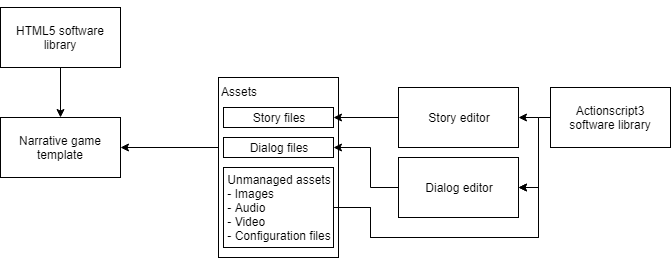
\includegraphics[width=0.75\textwidth]{StoryDialogEditorRelations}
    \caption{Story- en dialog editor relaties}
    \label{fig:editorrelations}
\end{figure}

\pagebreak
\section{Toekomst plannen}
\label{sec:editorfuture}
De toekomst van de editors zal, zoals in de inleiding beschreven, bestaan uit een web omgeving waarin meerdere personen tegelijk kunnen werken (collaborative editing). Hierin worden aanpassingen direct getoond aan teamleden wat het mogelijk maakt om met elkaar samen te werken aan dezelfde bestanden. Deze feature wordt nog interessanter wanneer klanten bij het ontwikkelproces betrokken worden. Zij zouden dan directe feedback of zelfs aanpassingen kunnen doen aan de game content. Het bedrijf geeft aan dat ze hier in de toekomst naar toe gaan werken, maar dat er meer onderzoek en resources nodig zijn om dit mogelijk te maken.

Hoewel dit vraagstuk niet in dit onderzoek past kan er wel rekening mee worden gehouden. Ook al zal het bedrijf voorlopig gebruik maken van een desktopapplicatie, moet er wel een blik op de toekomst geworpen worden. Bij het opzetten van een nieuwe editor vindt \organisation{} toekomstgerichtheid een belangrijk aspect; het bedrijf wil dan ook niet opnieuw een hele editor opzetten. Bij de keuzes die invloed hebben op de tech stack zal hier dan ook op worden gelet.

\pagebreak
\section{Pijnpunten in de huidige technology stack}
Beschikken over een stabiele en toekomstig gerichte tech stack is cruciaal voor een succesvol product. De tech stack heeft een directe invloed op de toegankelijkheid, schaalbaarheid en toekomstgerichtheid van de toekomstige editor. 

\subsection{Onzekerheid in de toekomst}
De huidige editors zijn gemaakt in Apache Flex. Dit is een omgeving waarin applicaties gemaakt kunnen worden met de hulp van ActionScript3 om logica te kunnen programmeren en MXML wat het definiëren van lay-outs toelaat in een XML-formaat\cite{WhatIsApacheFlex}. Projecten kunnen gecompileerd worden naar SWF-bestanden die kunnen worden uitgevoerd in een Flash- of Air run time. Vorig jaar, 25 juli, liet Adobe in een blog post weten dat ze ondersteuning voor Flash gaan beëindigen in 2020\cite{AdobeFlashFuture}. Hiernaast lijken er ook weinig updates plaats te vinden. Volgens de website van Apache Flex was de laatste update op 22 november 2017\cite{ApacheFlex}. Tenslotte werd Flash al eerder in meerdere populaire browsers standaard geblokkeerd vanwege veiligheidsredenen\cite{FlashWillBeBlocked}. Dit gaat tegen het toekomstbeeld van de editors in, het bedrijf wilt toewerken naar een webapplicatie. Verder leidt dit alles naar een onzekere toekomst van Apache Flex.

\subsection{Kleine community}
Het aanbod van libraries, klare oplossingen op veelvoorkomende problemen, is naar verhouding vrij minimaal omdat de community rond Apache Flex en ActionScript3 in vergelijking tot andere ontwikkelomgevingen relatief klein is. In de ‘populaire technologieën’ sectie van de enquête die Stack Overflow jaarlijks afneemt zijn Apache Flex en ActionScript3 niet te vinden\cite{StackOverflowSurvey2018}. Ondanks dat de Apache Flex community wel op Stack Overflow zit\cite{StackOverflowFlexQuestions}. Een kleinere community kan leiden tot minder hulp en een gebrek aan oplossingen voor veel voorkomende problemen. Dit is ook terug te zien aan ‘Flex Wires’, een library die de editors gebruiken om de nodes met lijnen aan elkaar te verbinden. De library is slecht aanpasbaar en biedt weinig functionaliteit. Verbindingen kunnen niet aangepast worden, er verschijnt altijd een grijze kromme lijn. Dit heeft als gevolg dat bepaalde features niet haalbaar zijn in de huidige editors. Hiernaast zitten er fouten in Flex Wires die alleen opgelost kunnen worden in de library zelf. Zo kunnen de verbindingen uit het niks verdwijnen, waardoor niet meer te zien is welke relaties er bestaan tussen nodes.

\subsection{Overtollige libraries}
Zowel de editors als het NGT maken gebruik van de \organisation{} software library welke generieke functionaliteiten en datastructuren bevat (zie \autoref{fig:editorrelations}). Echter moeten er twee libraries onderhouden worden omdat de huidige editors en het NGT geschreven zijn in verschillende programmeertalen. Het implementeren van nieuwe generieke functionaliteiten moet dubbel gedaan worden en de libraries moeten beide up-to-date zijn, omdat het NGT en de editors anders mogelijk niet meer goed samen kunnen werken.

\pagebreak
\section{Ontwikkelplatformen}
Het huidige ontwikkelplatform, Apache Flex, heeft een onzekere toekomst en sluit niet aan bij het toekomstbeeld van de editors die het bedrijf heeft. Het prototypen in een ontwikkelomgeving die die gericht op de toekomst is heeft meer waarde voor dit onderzoek.

\subsection{Aandachtspunten}
Bij het zoeken naar een gepast ontwikkelplatform werd er gelet op: de community om het platform heen, de toekomstgerichtheid van het platform en hoeveel werk het gaat kosten om deze te integreren in de huidige tech stack. Deze aspecten zijn gesorteerd op belang van hoog naar laag en worden hieronder vermeld met concrete vragen:

\begin{enumerate}
    \item Community
    \begin{itemize}
        \item Bestaat er een actieve community waarin mensen elkaar verder helpen met problemen?
        \item Zijn er bestaande oplossingen voor een visual scripting interface?
    \end{itemize}    
    \item Toekomstgerichtheid
    \begin{itemize}
        \item Door wie wordt het ontwikkelplatform onderhouden?
        \item Hoe ziet de toekomst van het ontwikkelplatform eruit?
        \item Kan er naast een desktopapplicatie ook uitgerold worden naar een web omgeving?
    \end{itemize}
    \item Integratie
    \begin{itemize}
        \item Sluit het ontwikkelplatform aan bij de rest van de tech stack?
        \item Sluit het ontwikkelplatform aan bij het bedrijf? Kunnen programmeurs overweg met het platform, zo niet hoe stijl is de leercurve?
    \end{itemize}
\end{enumerate}

\subsection{Selectie}
Er is een selectie gemaakt uit populaire en mogelijk passende ontwikkelplatformen:
\begin{enumerate}
    \item Haxe
    \item Electron
    \item NW
    \item Qt    
\end{enumerate}

\noindent Verder zullen de volgende ontwikkelplatformen kort worden behandeld, omdat deze potentie hadden maar al gauw niet de oplossing bleken te zijn.
\begin{enumerate}
    \item Unity
    \item Apache FlexJS
\end{enumerate}

\pagebreak
\subsubsection{Unity}
Het bedrijf wilt gebruik gaan maken van Unity voor de ontwikkeling van narrative games. Unity biedt een platform waarmee de verschillende disciplines in een projectteam beter samen kunnen werken. Het integreren van de nieuwe editor met Unity kan voordelen met zich meebrengen, zoals beter feedback en een betere workflow.
Echter is het niet aan te raden om een gehele editor in Unity te maken. Unity is van origine een game engine. Er kunnen simpele extensies gemaakt worden die getoond kunnen worden in Unity, maar een gehele narrative editor maken als Unity extensies vereist veel tijd. Hiernaast moeten extensies gemaakt worden op een manier die Unity afdwingt. Naast dat dit de oorzaak is van de grote hoeveelheid vereiste tijd brengt het ook limitaties met zich mee. Als de Unity API niet beschikt over een bepaalde benodigde functionaliteit is het niet mogelijk of gaat het erg veel tijd en creativiteit kosten.
Tenslotte heeft dit zware consequenties op de toekomst van de editor. Mocht het bedrijf ooit beslissen om van Unity weg te stappen dan zullen ze een deel van de editor opnieuw moeten ontwikkelen, omdat een groot deel van de code specifiek voor Unity geschreven zal zijn. Idealiter wilt het bedrijf niet afhankelijk zijn van Unity.

\subsubsection{Apache FlexJS}
Met de val van Flash is Apache een oplossing gaan zoeken om projecten van Apache Flex te compileren naar JavaScript. De oplossing die Apache heeft ontwikkeld heet Apache FlexJS, een variant op Apache Flex die code omzet naar JavaScript\cite{WhatIsApacheFlexJS}. Als \&ranj besluit componenten van de huidige editors te hergebruiken voor de nieuwe editors is het een optie om gebruik te maken van Apache FlexJS.
De nieuwe oplossing van Apache is echter nog niet getest in grotere applicaties en op de download pagina laat Apache weten dat er aardig wat features missen en bugs in zitten: “The Apache Flex team is pleased to offer this release, available as of 27 June 2017. Expect lots of bugs and missing features.”\cite{ApacheFlexJSDownload}. De laatste update was op 27 juni 2017, wat alweer bijna een jaar geleden is.
Tenslotte lijkt een groot deel van de web community al weg gestapt te zijn van Apache Flex en ActionScript3. Mogelijk omdat Apache niet snel genoeg met een oplossing kwam

\subsubsection{Haxe}
Haxe, een project dat gestart is op 22 oktober 2005, is een omgeving waarin applicaties geprogrammeerd kunnen worden in de Haxe programmeertaal. Deze programmeertaal is object georiënteerd, ‘strictly typed’ en de syntax lijkt op een mix tussen ActionScript3 en Java. Als de logica eenmaal geprogrammeerd is kan het ontwikkelplatform trans compileren, de Haxe programmeertaal omzetten, naar 12 verschillende programmeertalen\cite{CompilerTargetsHaxe}. De focus van Haxe lijkt dan ook te liggen op het ‘write once, run anywhere’ principe.

\textbf{Community}
Het open-source ontwikkelplatform lijkt klein maar actief. Dit blijkt uit fora en de aanwezigheid op social media\cite{HaxeCommunitySupport}. Hiernaast werd er op 3 tot 5 mei een Haxe bijeenkomst georganiseerd, waarin de community samen kwam en naar meerdere (gast)sprekers luisterde over de mogelijkheden die Haxe biedt\cite{HaxeSummit}. Deze bijeenkomsten, ook wel ‘summits’ genoemd worden gehouden sinds 2014\cite{HaxeSummitSince2014}, wat duidt op een vraag naar het ontwikkelplatform.
Hoewel de community aardig wat oplossingen en raamwerken heeft gecreëerd voor Haxe\cite{HaxeGithubTrending} mist er wel een oplossing voor een visual scripting interface die kan helpen bij het opzetten van de editors.

\textbf{Toekomstgerichtheid}
Het Haxe platform wordt ondersteund door een zo genaamde ‘Haxe Foundation’. Deze bestaat uit donaties en betaalde ondersteuningsabonnementen. De lijst van bedrijven die de ‘Haxe Foundation’ financieel ondersteunen bestaat uit 6 vrijwel onbekende bedrijven. Hiernaast is de roadmap die te vinden is op de website van Haxe vrij minimaal en achterhaald.
Doordat het ontwikkelplatform kan trans compileren naar 12 verschillende programmeertalen, waaronder Javascript, betekent dit wel dat er zowel desktopapplicaties als webapplicaties kunnen worden uitgerold.

\textbf{Integratie}
De huidige tech stack komen de Javascript en Actionscript programmeertalen terug. Hoewel de Haxe programmeertaal inspiratie heeft genomen van ActionScript3 kan het wel tijd kosten om de taal te leren. Hiernaast zal er kennis vergaart moeten worden van het ontwikkelplatform zelf en er zal een nieuwe deployment pipeline opgezet moeten worden.
Om de software library te kunnen gebruiken zal er een tussen laag geprogrammeerd moeten worden, zoals dit staat beschreven in de handleiding\cite{HaxeUsingExternalJavaScriptLibraries}.

\subsubsection{Electron}
Wat begon op 15 juli 2013 als een project genaamd ‘atom shell’\cite{StartOfAtomShell} die ter ondersteuning diende voor de populaire tekst bewerker genaamd ‘atom editor’\footnote{https://atom.io/}, is sinds 23 april 2015 bekend als Electron\cite{AtomShellIsNowElectron}. Dit raamwerk is open-source en geeft ontwikkelaars de mogelijkheid om cross-platform desktop apps te creëren met behulp van webtechnologieën, zoals HTML, CSS en JavaScript. Om dit alles mogelijk te maken faciliteert Electron Chromium\footnote{https://www.chromium.org/} (het browser project achter de populaire Chrome browser) en NodeJS\footnote{https://nodejs.org/}, een cross-platform JavaScript run-time omgeving. 

\textbf{Community}
Naast dat het project op GitHub 2.636 volgers, 59.906 favorieten en 7.844 forks\footnote{Een ‘fork’ is een copy van andermans project en wordt meestal gebruikt als startpunt van eventuele uitbreidingen en aanpassingen.}\footnote{Gemeten op: 11-05-2018 17:09} \cite{GithubElectron} heeft, weet Electron een gigantische community om zich heen te vormen door webtechnologieën en web ontwikkelaars te betrekken. Volgens het onderzoek naar ontwikkelaars van StackOverflow blijkt dat JavaScript, HTML en CSS de meest populaire technologieën van 2018 zijn\cite{StackOverflowAnnualSurvey2018}. JavaScript is al 6 jaar de meest gebruikte programmeertaal volgens de StackOverflow onderzoeken. Hiernaast wordt NodeJS het meest gebruikt van alle frameworks, libraries en tools\cite{StackOverflowAnnualSurvey2018}.
De populariteit van Javascript en NodeJS leidt tot vele diagramming libraries die een bestaande oplossing bieden op een visual scripting interface. Het is wenselijk om te beschikken over bestaande oplossingen die direct toepasbaar zijn, zodat het wiel niet opnieuw uit gevonden hoeft te worden.

\textbf{Toekomstgerichtheid}
Electron wordt onderhouden door GitHub\footnote{https://github.com/} een platform waarop software beheerd kan worden door middel van versie beheer (git). Github zegt te beschikken over een community van 27 miljoen mensen, gemeten in maart 2018\cite{GithubAbout}. Hiernaast biedt het platform opslag voor 80 miljoen verschillende softwareprojecten.
Verder wordt Electron gebruikt door bekende desktopapplicaties zoals: Skype, GitHub Desktop, Visual Studio Code, Slack en Atom\cite{ElectronJS}.
Door tijdens het ontwikkelproces van de editors een duidelijke scheiding te maken tussen de applicatie en Electron kan de toekomstgerichtheid bevorderd worden. De applicatie zonder Electron blijft een webapplicatie, wat betekend dat deze relatief makkelijk omgezet kan worden naar een web omgeving. Dit sluit goed aan bij de toekomstvisie van \&ranj besproken in \autoref{sec:editorfuture}.

\textbf{Integratie}
In de huidige tech stack wordt er veel gewerkt met JavaScript. Een groot probleem, zoals eerder, besproken zijn de overtollige software libraries. Deze libraries bevatten herbruikbare componenten voor zowel het NGT als de huidige editors. Echter zijn het NGT en de huidige editor ontwikkeld in verschillende programmeertalen, JavaScript en ActionScript3, waardoor er 2 verschillende versie bijgehouden moeten worden. Het overstappen van ActionScript naar JavaScript kost wat werk, maar omdat de syntax van ActionScript geïnspireerd is door Javascript zal het proces soepeler kunnen verlopen.
Door over te stappen naar Electron en ActionScript uit te sluiten hoeft de ActionScript library van \&ranj niet meer onderhouden te worden; er kan gebruik worden gemaakt van de JavaScript software library. Herbruikbare componenten bevinden zich hierdoor dan in één library.

\pagebreak
\subsubsection{NW}
NW.js, eerder bekend als ‘node-webkit’, is een open source run-time gebaseerd op Chromium en NodeJS. Het biedt de mogelijkheid om NodeJS modules direct aan te roepen in HTML-bestanden. Deze run time is erg vergelijkbaar met Electron in de zin dat ze beide een relaties hebben tot Chromium en NodeJS.

\textbf{Community}
Het GitHub project van NW.js heeft op het moment\footnote{Gemeten op: 11-05-2018 17:09} 1.812 volgers, 33.689 favorieten en 3.745 forks\cite{NWGitHub}. Om de community samen de brengen heeft NW.js een Gitter\footnote{https://gitter.im/nwjs/nw.js}, wat fungeert als een chatroom, opgezet waarin de community met elkaar kan praten en elkaar verder kan helpen. Hiernaast lijkt de community aanwezig te zijn op StackOverflow\cite{StackOverflowNW}.
Vanwege de grote community rondom web development met onder andere Javascript als veelgebruikte programmeertaal bestaan er genoeg libraries waarmee een visual scripting interface opgezet kan worden.

\textbf{Toekomstgerichtheid}
NW.js wordt gesponsord door Intel\footnote{https://www.intel.com/}, maar uit data van Github\footnote{https://github.com/nwjs/nw.js/graphs/contributors} blijkt dat er vooral één persoon actief aan werkt. Het project blijkt slow but steady uitgebreid te worden.
Er zijn een groot aantal applicaties gemaakt met NW.js\cite{NWJSApps}. De meest bekende is misschien wel de WhatsApp desktopapplicatie. Echter kwam deze applicatie ook naar boven in de lijst van Electron applicaties. Na de Whatsapp desktopapplicatie gedownload te hebben blijkt dat deze Electron gebruikt, wat te zien is aan de bestand structuur van de applicatie en het overduidelijke ‘electron.asar’ bestand.
Een NW.js applicatie is net zoals Electron een browser in een desktopapplicatie. Als er tijdens het ontwikkelingsproces een duidelijke scheiding wordt gelegd tussen de applicatie zelf en NW.js kan dezelfde met relatief kleine moeite ook ingezet worden als webapplicatie. Ook dit slaat goed aan bij de toekomst van de editors zoals beschreven in \autoref{sec:editorfuture}.

\textbf{Integratie}
Net zoals Electron zal NW de ActionScript3 library overbodig maken, waardoor alleen nog de JavaScript library onderhouden hoeft te worden. Het overstappen zal wat werk kosten, maar relatief makkelijk zijn vanwege de overeenkomsten tussen de ActionScript3 en JavaScript syntax.
Programmeurs binnen het bedrijf zijn meer bekend met JavaScript dan ActionScript3 wat het overstappen naar JavaScript makkelijker kan maken voor de ontwikkelaars.

\pagebreak
\subsubsection{Qt}
Qt is een raamwerk waarin crossplatform applicaties kunnen worden ontwikkeld. Hiernaast biedt het raamwerk een manier om graphical user interfaces (GUI) op te zetten\cite{Qt}. Qt is geschreven in C++, maar ontwikkelaars kunnen ook gebruik maken van andere programmeertalen\cite{QtLanguageBindings}. Echter wordt er aangeraden om in C++ te ontwikkelen.

\textbf{Community}
De Qt community is actief op StackOverflow\cite{StackOverflowQtQuestions} en het Qt forum\cite{QtForum}. Vooral op het Qt forum is de community actief. Hiernaast organiseert Qt jaarlijkse summits en Qt dagen.  
Er zijn geen libraries gevonden die kunnen helpen bij het opzetten van de visual scripting interface. Wel heeft Qt een voorbeeldje opgezet waarmee dit eventueel bereikt zou kunnen worden\cite{QtDiagramExample}. Dit neemt echter niet weg dat het veel werk zal gaan kosten.

\textbf{Toekomstgerichtheid}
Qt wordt ontwikkeld en onderhouden door het bedrijf zelf en biedt een open source en commerciële versie van het raamwerk\cite{QtLicense}. Verder maken bekende bedrijven zoals Valve\cite{ValveQt}, Blizzard\cite{BlizzardQt}, VideoLan\cite{VideoLanQt} en AMD\cite{AMDQt} gebruik van Qt. Wat er op duidt dat Qt over een goed getest ontwikkelplatform beschikt.
Er is een mogelijkheid om webapplicaties te ontwikkelen in Qt\cite{QtWebKit}\cite{QtCutelyst}\cite{WtQt}. Echter is het niet duidelijk of dezelfde codebase gebruikt kan worden voor zowel web- als desktopapplicatie.

\textbf{Integratie}
Als raamwerk geschreven in c++ past het minder goed bij een tech stack die vooral bestaat uit webtechnologieën. Hiernaast is het voor de editors lastig om voordeel te halen uit een low level programmeertaal zoals c++, omdat deze de fijne controle die c++ biedt niet benutten. De editors profiteren niet van kleine beetjes extra prestatie op het gebied van snelheid, omdat het slecht een tool is; het spel wordt uiteindelijk gebouwd in het NGT.
De huidige tech stack die alleen bestaat uit high level programmeertalen resulteert in programmeurs die hier goed mee op weg kunnen. Om vervolgens een low level programmeertaal, zoals c++, te introduceren kan lastig zijn zonder programmeurs met ervaring.

\pagebreak
\subsubsection{NW vs Electron}
NW en Electron lijken beide hetzelfde doel te delen: desktopapplicaties ontwikkelen in HTML, CSS en JavaScript. Echter blijkt Electron de populairdere optie te zijn van de twee. Dit blijkt uit de statistieken van GitHub (zie \autoref{tab:NWvsElectron}). Hiernaast laat een analyse tool genaamd “IS IT MAINTAINED?”\footnote{http://isitmaintained.com} zien dat er een significant verschil zit in de snelheid waarop vraagstukken van gebruikers beantwoord worden.

\begin{table}[htb]
    \centering
    \begin{tabular}{ | l | l | l | }
        \hline
        GitHub statistieken & \textbf{NW} & \textbf{Electron} \\
        \hline
        Volgers (Watches) & 1.812 & \cellcolor{green!15}2.636 \\
        \hline
        Favorieten (Stars) & 33.689 & \cellcolor{green!15}59.906 \\
        \hline
        Forks & 3.745 & \cellcolor{green!15}7.844 \\
        \hline
        Bijdragers (Contributors) & 98 & \cellcolor{green!15}751 \\
        \hline
        Gemiddelde oplossingstijd van gestelde vraagstukken & \cellcolor{orange!25}5 dagen & \cellcolor{green!15}22 uur \\
        \hline
        Open vraagstukken & \cellcolor{red!25}29\% & \cellcolor{green!15}5\% \\ 
        \hline
    \end{tabular}
    \caption{NW vs Electron (Gemeten op: 11-05-2018 17:09)}    
    \label{tab:NWvsElectron}
\end{table}

Zowel NW als Electron kunnen worden beschouwd als battle tested\cite{NWJSApps}\cite{ElectronApps}. Hiermee wordt bedoeld dat er meerdere applicaties bestaan die ontwikkeld zijn in deze ontwikkelplatformen. Echter zijn de meeste applicaties ontwikkeld in Electron, voorbeelden hiervan zijn: ‘Visual Studio Code’\footnote{https://code.visualstudio.com/}, ‘Slack’\footnote{https://slack.com/}, ‘Atom’\footnote{https://atom.io/} en ‘Discord’\footnote{https://discordapp.com/}.

In het gebruik van de ontwikkelplatformen zit er naast de API ook een verschil in het entry point. Beide definiëren het ingangspunt van de applicatie in het package.json bestand. In NW kan dit zowel een HTML-bestand als een JavaScript bestand zijn. Electron dwingt het gebruik van een JavaScript bestand af om meer controle te bieden over het frame waarin de applicatie zich bevindt.

Tenslotte viel er iets op aan de statistieken van GitHub. Hieraan is te zien dat een persoon met de gebruikersnaam “zcbenz” tussen 2012 en 2013 relatief actief was op het NW-project. Na deze periode is deze persoon, Cheng Zhao, gaan werken aan Electron. Cheng Zhao heeft gewerkt aan NW tijdens zijn stageperiode. Hij beschrijft Electron als een tweede poging op NW\cite{FromNWToElectronZhaoCheng}. 

\subsection{Deel conclusie en aanbevelingen}
De mogelijkheid om desktopapplicaties te kunnen ontwikkelen door middel van webtechnologieën is ideaal voor het bedrijf. Het sluit goed aan bij de toekomst van de editors, omdat deze met minimale aanpassingen in een web omgeving kunnen worden geplaatst. Verder biedt de community rondom JavaScript oplossingen voor de interface van de editors. Dit kan helpen bij het ontwikkelproces van de nieuwe editor en voorkomt het maken van al bestaande oplossingen. Tenslotte past een JavaScript raamwerk goed in de huidige tech stack, omdat dit het makkelijker maakt om met de JavaScript software library van \&ranj te communiceren. Daarnaast werkt het bedrijf vaak met JavaScript waardoor programmeurs bekend zijn met de programmeertaal.

Zowel Electron als NW laten het ontwikkelen van desktopapplicaties met behulp van webtechnologieën toe. Echter is de community rondom Electron groter, wat mogelijk komt door de ondersteuning van GitHub. Hiernaast biedt de ondersteuning van GitHub en het aantal populaire applicaties de zekerheid dat Electron voorlopig zal blijven bestaan. Tenslotte lost Electron sneller vraagstukken van gebruikers op.

Dit neemt niet weg dat NW niet zou kunnen werken in deze context. Het is niet rechtvaardig om dit ontwikkelplatform compleet af te schrijven. Om zeker te zijn van een juiste keuze zou er een demo gemaakt kunnen worden in zowel NW als Electron. Beide zullen hoogstwaarschijnlijk geen limitatie stellen aan de editor, omdat deze weinig gebruik maakt van native APIs. Vanwege het gebonden tijdslimiet aan dit onderzoek zal er gekozen worden voor Electron. Deze keuze is gemaakt op het gebied van community en toekomstgerichtheid; Electron heeft een grotere community om zich heen en met de ondersteuning van GitHub zal het product voorlopig blijven bestaan.

\section{User interface}
De user interface (UI) synchroon houden met de achterliggende staat kan erg rommelig en lastig zijn in standaard HTML en JavaScript. Code wordt al gauw onleesbaar en bij een kleine verandering in de staat van de applicatie wordt heel de UI geüpdatet. Om dit probleem op te lossen hebben meerdere bedrijven JavaScript UI libraries en raamwerken opgezet. Deze oplossingen delen de UI op in componenten waarin zich component specifieke logica bevindt; componenten bevorderen de encapsulatie van logica. Verder kunnen deze componenten, als de logica erachter goed ingekapseld is, in andere componenten gebruikt worden. Dit resulteert in een manier om een houdbare en flexibele UI op te zetten.

\subsection{User interface van de huidige editors}
De UI van de huidige editors kan worden opgedeeld in componenten met ieder haar eigen functionaliteit. Al deze UI-componenten bevinden zich op één pagina. De story- als dialog editor lijken te beschikken over vrijwel dezelfde (hoofd)componenten:
\begin{enumerate}
    \item Inspector
    \item Toolkit
    \item Tabs
    \begin{enumerate}
        \item Canvas
    \end{enumerate}
\end{enumerate}

\begin{figure}[H]
    \begin{minipage}[b]{0.45\textwidth}
        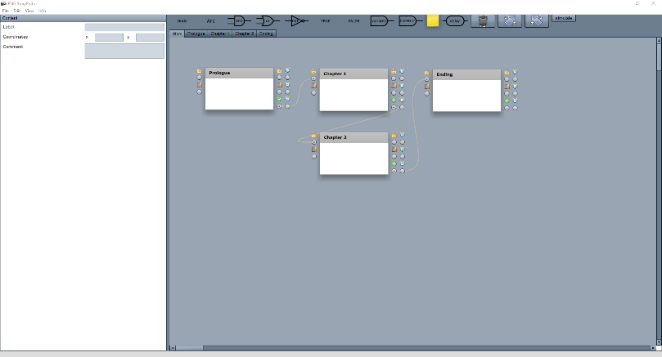
\includegraphics[width=\textwidth]{StoryEditor_SimpleStory}
        \caption{Story Editor interface}
        \label{fig:storyeditorinterface}
    \end{minipage}
    \hfill
    \begin{minipage}[b]{0.45\textwidth}
        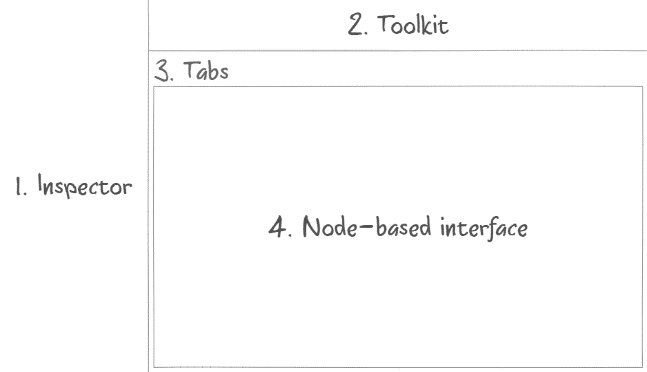
\includegraphics[width=\textwidth]{StoryEditor_ComponentWireFrame}
        \caption{Editor componenten}
        \label{fig:storyeditorcomponents}
    \end{minipage}
\end{figure}

Er bevindt zich een miniem aantal componenten op een enkele pagina. Dit duidt op de behoefte aan een kleine user interface library zonder navigatie functionaliteit.

% \begin{figure}[htb]
%     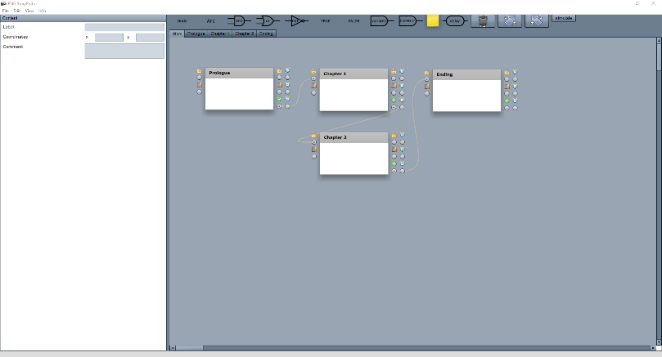
\includegraphics[width=\textwidth,height=\textheight,keepaspectratio]{StoryEditor_SimpleStory}
%     \caption{Story Editor interface}
%     \label{fig:storyeditorinterface}
%     \centering
% \end{figure}

% \begin{figure}[htb]
%     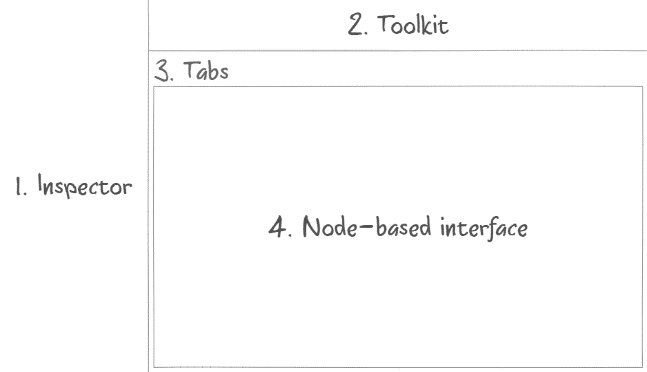
\includegraphics[width=\textwidth,height=\textheight,keepaspectratio]{StoryEditor_ComponentWireFrame}
%     \caption{Editor componenten}
%     \label{fig:storyeditorcomponents}
%     \centering
% \end{figure}

\clearpage
\subsection{User interface frameworks \& libraries}
Er zijn meerdere oplossingen beschikbaar voor het maken van user interfaces. Sommige bestaan uit een compleet raamwerk en een dwingen een bepaalde manier van werken af. Er kan gezegd worden dat deze een grote eigenzinnigheid hebben. Andere oplossingen zijn kleine libraries die zich alleen focussen op het inkapselen van componenten.

\subsubsection{Aandachtspunten}
Bij het zoeken naar een passende oplossing wordt er gekeken naar de volgende punten:
\begin{enumerate}
    \item De omvang van het ecosysteem
    \item Eigenzinnigheid
    \item Toekomstgerichtheid
    \begin{itemize}
        \item Wie onderhoudt/ steunt het project?
        \item Welke (populaire) producten gebruiken deze oplossing?
    \end{itemize}
    \item Snelheid
    \item Leercurve    
\end{enumerate}

\subsubsection{Verwachtingen}
Er wordt gezocht naar een oplossing waarmee componenten in gekapseld kunnen worden. Een ecosysteem met meerdere doeleinden kan worden beschouwd als overbodig. Zo bestaan de huidige editors uit één scherm wat een router\footnote{Een klasse die verantwoordelijk voor navigatie binnen een applicatie} overbodig maakt. Daarom zou een ecosysteem met een router redundant zijn.

Omdat er slechts gezocht wordt naar een component gebaseerde oplossing is het gewenst dat het raamwerk of de library vrijwel niet eigenzinnig is.

Verder is het belangrijk dat de ontwikkeling van het product actief is en dat deze niet snel zal verdwijnen. Een voorspelling kan gedaan worden op basis van (populaire) applicaties die het product gebruiken en of er (grote) bedrijven zijn die het product onderhouden of steunen.

Tenslotte zijn de snelheid en leercurve van het product minder belangrijk voor dit probleem, mits deze niet enorm afwijken van de rest. Bij de editor zal flexibiliteit en toekomstgerichtheid boven snelheid gaan. Hiernaast zal het ontwikkelen van een nieuwe editor moeten resulteren in een toekomstgerichte oplossing die nog voor jaren gebruik zal kunnen worden. Dit maakt het minder erg als de leercurve van het product iets hoger ligt.

\subsubsection{Selectie}
Om de staat van de applicatie synchroon te houden met de UI kan er gebruik worden gemaakt van bestaande oplossingen. Er is een selectie gemaakt uit populaire user interface raamwerken en libraries:
\begin{itemize}
    \item Vue
    \item Angular
    \item React
    \item Ember    
\end{itemize}

\pagebreak
\subsubsection{Resultaten}
De geselecteerde oplossingen zijn geanalyseerd op de eerdergenoemde aandachtspunten. Het resultaat wordt weergeven in \autoref{tab:uiframeworks}.

\begin{table}[htb]
    \centering
    \begin{tabular}{ l | p{2.5cm} p{2.5cm} p{2.5cm} p{2.5cm} }
    & \textbf{Vue}\footnote{https://vuejs.org/} & \textbf{Angular}\footnote{https://angular.io/} & \textbf{React}\footnote{https://reactjs.org/} & \textbf{Ember}\footnote{https://www.emberjs.com/}\\
    \hline
    \textbf{GitHub stats (05/03/2018)} & & &\\
    Volgers & 4.561 & 2.918 & 5.566 & 1.040\\
    Favorieten & 85.500 & 33.694 & 89.726 & 18.682\\
    Forks & 12.545 & 8.275 & 16.971 & 3.850\\
    \textbf{Gebacked door} & 1 persoon, Yuxi (Evan) You &Google & Facebook & LinkedIn, Netflix\\
    \textbf{"Native" language} & JavaScript & Typescript\footnote{TypeScript is een getypeerde ‘superset’ van JavaScript. Geschreven TypeScript code compileert naar JavaScript.} & JavaScript & JavaScript\\
    \textbf{TypeScript ondersteuning} & Ja, er zijn typing beschikbaar &Ja, out of the box & Ja, er zijn typing beschikbaar + typescript CLI\footnote{Command line interface tooling} & Ja, er zijn typing beschikbaar + typescript CLI\\
    \textbf{Ecosysteem} & Modulair, o.a. router, state management, cli, RxJS integration & Modulair, o.a. router, state management, cli, RxJS integration &	Modulair. Ecosysteem opgebouwd door community (e.g. community router) & Modulair, o.a. router, state management, cli\\
    \textbf{Leercurve} & \cellcolor{green!15}Makkelijk, door de flexibiliteit die Vue biedt & \cellcolor{red!25}Lastiger door de grote eigenzinnigheid dat het framework kent & \cellcolor{green!15}Makkelijk, het is een relatief kleine library & \cellcolor{red!25}Lastiger door de grote eigenzinnigheid dat het framework kent\\
    \textbf{Snelheid}\footnote{http://www.stefankrause.net/js-frameworks-benchmark7/table.html} & \cellcolor{green!15}Snel, Virtual DOM & \cellcolor{green!15}Snel & \cellcolor{green!15}Snel, Virtual DOM & \cellcolor{red!25}Langzaam\\
    \textbf{Eigenzinnigheid} & \cellcolor{green!15}Klein & \cellcolor{red!25}Groot, je moet in de kaders van angular werken & \cellcolor{green!15}Klein & \cellcolor{red!25}Groot\\
    \end{tabular}
    \caption[]{Inventarisatie van user interface frameworks en libraries \footnotemark}
    \label{tab:uiframeworks}
\end{table}
\footnotetext{Voor het laatst ingezien op: 05/03/2018}

\pagebreak
\subsubsection{Virtual DOM}
In het verleden waren webapplicaties statisch en relatief klein. Tegenwoordig wordt er veel gewerkt met (grotere) single page applications (SPA). Een SPA bestaat uit kleine individuele componenten die met elkaar kunnen communiceren en los van elkaar geüpdatet of vervangen kunnen worden\cite{SPA}. De webpagina wordt nooit in zijn geheel ververst of herladen. Hiernaast is een SPA verantwoordelijk voor het correct afhandelen van gebruikersinvoer.
Webapplicaties moet constant het document object model (DOM) achter de webpagina veranderen om feedback te kunnen tonen aan de gebruiker nadat deze input heeft geleverd. Voor grotere SPA-webapplicaties is dit een probleem, omdat DOM bestaat uit een boom. De nodes van de DOM boom zijn makkelijk af te gaan, maar in een grotere boom structuur (zoals in grote SPA applicaties) wordt dit al gauw een langdurig proces.
Hier komt virtual DOM in het spel. Dit is een abstractie van de ‘traditionele’ DOM\cite{Psaila2008}. Veranderingen in de virtual DOM resulteren in de executie van een verschil algoritme. Het resultaat van dit algoritme wordt vervolgens gereflecteerd in de “echte” DOM, waarin alleen de veranderde nodes aangepast worden. Door delen aan te passen in plaats van de gehele DOM kan de webapplicatie sneller reflecteren op de input van de gebruiker.
Zowel Vue als React maken gebruik van Virtual DOM.

\subsubsection{TypeScript}
Uit een onderzoek naar code kwaliteit op GitHub blijkt dat strongly typed programmeertalen minder gevoelig zijn voor fouten dan loosly typed programmeertalen\cite{Ray2014}. JavaScript is een voorbeeld van een loosly typed programmeertaal. Om code kwaliteit te verhogen en menselijke fouten te voorkomen wordt er geadviseerd om gebruik te maken van een strongly typed programmeertaal. Volgens onderzoek naar code kwaliteit op GitHub worden er minder fouten gemaakt in TypeScript projecten\cite{Ray2014}. TypeScript is een strongly typed superset van JavaScript, wat betekent dat TypeScript code gecompileerd kan worden naar JavaScript. Dit proces wordt ook wel transpiling genoemd.

TypeScript is ontwikkeld en wordt onderhouden door Microsoft. Hiernaast lijkt bijna iedere JavaScript library ondersteuning te bieden door typings aan te bieden. Typings zijn bestanden die TypeScript gebruikt om onderscheid te maken tussen verschillende types. Via deze typings kunnen JavaScript libraries samen werken met TypeScript code. 
Er is verder geen onderzoek gedaan naar alternatieven naast TypeScript, zo zou Flow\footnote{https://flow.org/} ook een oplossing kunnen zijn.

\subsection{Deel conclusie en aanbeveling}
Er wordt gezocht naar een kleine library die zich bezighoudt met het inkapselen van componenten. Alle vier de oplossingen beschikken over een modulair ecosysteem, maar React steekt hier bovenuit. React is een library wat betekend dat deze een relatief kleine omvang heeft in tegenstelling tot de andere oplossingen die gezien worden als frameworks. De oplossing van Facebook, React, regelt de synchronisatie tussen ingekapselde componenten en de staat van de applicatie.

Vue is een opkomende technologie die naast React ook een potentiele oplossing kan zijn. Net zoals React maakt Vue gebruik van virtual DOM, wat voor beide een positief effect op de snelheid waarmee componenten geüpdatet en vervangen worden. Hiernaast dwingen ze allebei geen strikte werkwijze af; ze kennen allebei een kleine eigenzinnigheid. Het ecosysteem van Vue biedt zelf meer “out of the box” functionaliteiten en heeft een bredere focus. Ondanks dat React zich alleen bezighoudt met het inkapselen van componenten heeft de community rondom React een eigen ecosysteem om React heen gebouwd.

Omdat er wordt gezocht naar een relatief kleine library die het mogelijk maakt om componenten te kunnen specificeren, is React in deze context een beter passende oplossing. React heeft een nauwe focus waar Vue een bredere focus heeft. Hiernaast wordt React gebruikt in producten van Facebook, Netflix\cite{NetflixReact} en in 2817+ andere tech stacks\footnote{https://stackshare.io/react/in-stacks}; de library heeft zichzelf bewezen. Vue is wat nieuwer en ondanks de toenemende populariteit wordt het minder gebruikt.

\section{Visual scripting interface}
Het doel van zowel de huidige als de nieuwe editor is om niet-programmeurs de game content aan te kunnen laten passen. Door gebruik te maken van een visual scripting interface kan de game content aangepast worden zonder enige programmeerkennis\cite{VisualScripting}. Stukken game content worden gezien als objecten met een visuele weergave die ook wel “nodes” genoemd worden. De eigenschappen van deze objecten kunnen vervolgens aanpast worden in de editor zelf.

Door nodes met elkaar te verbinden kan de gebruiker zonder een enkele lijn code het narratief moduleren.

\subsection{Diagramming libraries}
Visual scripting wordt toegepast op verschillende platformen\cite{UnityAssetStoreVisualScripting}\cite{NoFlo}\cite{GitHub3dVisualScripting}. Het wiel hoeft niet opnieuw uitgevonden te worden; bestaande oplossingen kunnen gebruikt worden voor het visualiseren van de nodes. Deze oplossingen gaan onder de naam ‘diagramming libraries’ omdat ze meestal gebruikt worden voor het tekenen van diagrammen. Er kan gebruik gemaakt worden van deze libraries om nodes te visualiseren.

\subsection{Eisen}
Voordat er een selectie aan libraries is gemaakt zijn er eisen opgesteld. Deze zijn gebaseerd op het MoSCoW principe. De eisen zijn verdeeld onder de volgende categorieën:

\begin{itemize}
    \item \textbf{M}ust have; randvoorwaarden en functionele eisen, vereist voor het product
    \item \textbf{S}hould have; operationele eisen met groot belang, behoeftes van het product
    \item \textbf{C}ould have; operationele eisen, behoeftes van het product
    \item \textbf{W}ould have; ontwerpbeperkingen, principes en (code)kwaliteitsbewaking
\end{itemize}

\subsubsection{Must have; de library moet}
\begin{itemize}
    \item Voorzien zijn van documentatie
    \item Restricties kunnen leggen op connecties tussen porten
    \item Nodes in elkaar kunnen voegen
    \item Nodes kunnen highlighten
    \item Controls (zoals input velden) op nodes kunnen leggen
\end{itemize}

\subsubsection{Should have; het is van belang dat de library}
\begin{itemize}
    \item Nodes kunnen copy/ pasten*
    \item Acties ongedaan kunnen maken*
    \item Een navigeerbaar canvas aanbieden**
    \item Group selectie mogelijk maakt*
    \item De mogelijkheid biedt om grafen in grafen in te kunnen maken (sub-graphs).
\end{itemize}

\subsubsection{Could have; het is mooi meegenomen als de library}
\begin{itemize}
    \item Een minimap kan tonen waarop alle nodes zichtbaar zijn
    \item Real-time collaboratie toelaat
    \item De nodes kan ordenen
    \item De nodes snapt op een raster
    \item Een zoekfunctie biedt
    \item Een verschil algoritme implementeert
    \item Het groeperen van nodes mogelijk maakt
\end{itemize}

\subsubsection{Would have; om de houdbaarheid van het product te verhogen moeten de library}
\begin{itemize}
    \item Typings aanbieden
\end{itemize}

\noindent \textit{* zou eventueel zelf met relatief weinig moeite geïmplementeerd kunnen worden}\\
\textit{** er kan gebruik gemaakt worden van andere oplossingen voor dit probleem}\footnote{https://github.com/ariutta/svg-pan-zoom}

\subsubsection{Selectie en analyse}
Er is een selectie gemaakt uit JavaScript diagramming libraries:
\begin{itemize}
    \item D3-node-editor\footnote{https://github.com/Ni55aN/d3-node-editor}
    \item wcPlay\footnote{https://github.com/WebCabin/wcPlay}
    \item JointJS\footnote{ https://github.com/clientIO/joint}
    \item JointJS + Rappid (commerciële versie van JointJS)\footnote{https://www.jointjs.com/}
    \item MxGraph\footnote{https://github.com/jgraph/mxgraph}
    \item GoJS\footnote{https://gojs.net/latest/index.html}
\end{itemize}

\noindent De selectie aan diagramming libraries is afgezet tegen de opgestelde eisen en op genomen in \autoref{tab:diagramminglibraryfunctionality}.

% \begin{landscape}
    \begin{sidewaystable}[p]
        % 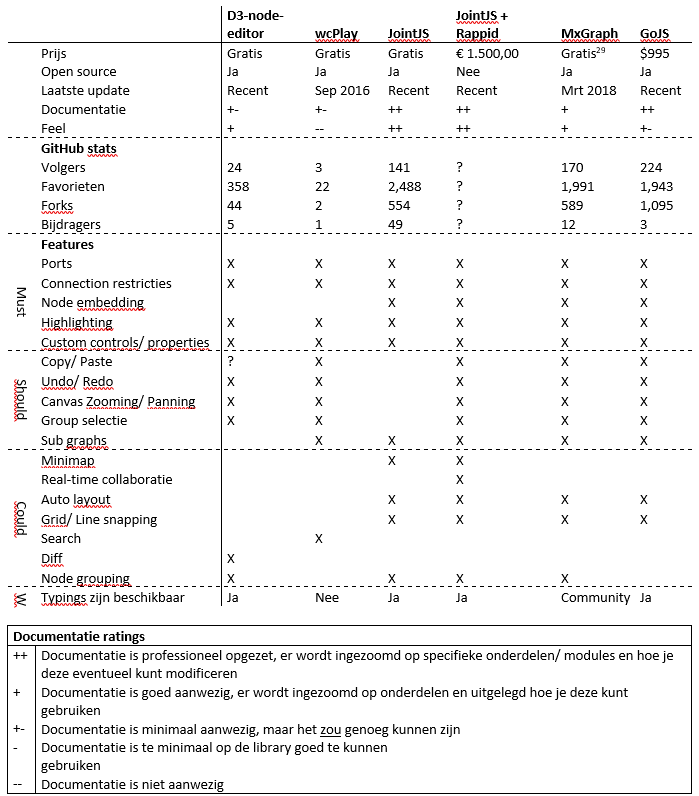
\includegraphics[width=\textwidth]{DiagrammingLibraryMatrix}
        \centering
        \resizebox{.82\columnwidth}{!}{
            \begin{tabular}{ l l | l l l l l l }
                \ & \ & \textbf{D3-node-editor} & \textbf{wcPlay} & \textbf{JointJS} & \textbf{JointJS + Rappid} & \textbf{MxGraph} & \textbf{GoJS}\\ \hline
                & Prijs & Gratis & Gratis & Gratis & \euro 1500 & Gratis & \euro 995 \\
                & Open source & Ja & Ja & Ja & Nee & Ja & Ja  \\ 
                & Laatste update & Recent & Sep 2016 & Recent & Recent & 01/03/2018 & Recent  \\
                & Documentatie & +-- & +-- & ++ & ++ & + & ++  \\
                & Feel & + & -- -- & ++ & ++ & + & +-- \\ \hdashline
                & \textbf{GitHub stats (16/05/2018)} &  &  &  &  &  &  \\ 
                & Volgers & 24 & 3 & 141 & - & 170 & 224 \\
                & Favorieten & 358 & 22 & 2.488 & - & 1.991 & 1.943 \\
                & Forks & 44 & 2 & 554 & - & 589 & 1.095 \\
                & Bijdragers & 5 & 1 & 49 & - & 12 & 3 \\ \hdashline
                & \textbf{Features} &  &  &  &  &  & \\
                \multirow{5}{*}{Must} & Ports & X & X & X & X & X & X \\ 
                & Connection restricties & X & X & X & X & X & X \\
                & Node embedding &  &  & X & X & X & X \\
                & Highlighting & X & X & X & X & X & X \\
                & Custom controls/ properties & X & X & X & X & X & X \\ \hdashline
                \multirow{5}{*}{Should} & Copy/ Paste & ? & X &  & X & X & X \\
                & Undo/ Redo & X & X &  & X & X & X \\
                & Canvas Zooming/ Panning & X & X &  & X & X & X \\
                & Group selectie & X & X &  & X & X & X \\
                & Sub graphs &  & X & X & X & X & X \\ \hdashline
                \multirow{6}{*}{Could} & Minimap &  &  & X & X &  &  \\
                & Real-time collaboratie &  &  &  & X &  &  \\
                & Auto layout &  &  & X & X & X & X \\
                & Grid/ Line snapping &  &  & X & X & X & X \\
                & Search &  & X &  &  &  &  \\
                & Diff & X &  &  &  &  &  \\
                & Node grouping & X &  & X & X & X &  \\ \hdashline
                \multirow{1}{*}{Would} & Typings zijn beschikbaar & Ja & Nee & Ja & Ja & Community & Ja \\
            \end{tabular}
        }
            
        \caption[]{Diagramming libraries en hun functionaliteiten (Voor het laatst ingezien op: 16/05/2018)}
        \label{tab:diagramminglibraryfunctionality}
    \end{sidewaystable}
    % \footnotetext{Voor het laatst ingezien op: 16/05/2018}
% \end{landscape}

\subsection{Deel conclusie en aanbevelingen}
Uit de analyse blijkt dat ‘D3-node-editor’ en ‘wcPlay’ niet voldoen aan de randvoorwaarden. Dit lag vooral aan de matige documentatie die de libraries meeleveren. Hierdoor is het erg lastig om de libraries toe te passen.

MxGraph en Rappid beschikken beide over een grote feature set die voldoen aan de requirements die vooraf opgesteld zijn. MxGraph was voorheen een commerciële oplossing, maar is nu gratis te gebruiken. Rappid met JointJS is de betaalde optie met collaborative editing functionaliteit. Hiernaast lijkt de community rondom JointJS groter; de library lijkt populairder te zijn dan MxGraph.

De commerciële optie, Rappid met JointJS, komt met betere documentatie en mogelijke ondersteuning. Dit kan essentieel zijn bij het opzetten van de editors. De collaborative editing functionaliteit van Rappid zou eventueel ook interessant kunnen zijn voor het bedrijf.

In het prototype is er gekozen voor de optie die voldoet aan de meeste eisen: JointJS + Rappid. Daarentegen is Rappid betaald en er zal daarom in het prototype gewerkt worden met JointJS. Deze voldoet aan de randvoorwaarden en biedt genoeg functionaliteit om het prototype te ondersteunen. Rappid is een laag bovenop JointJS en zou eventueel later toegevoegd kunnen worden.

\section{Conclusie}
Met dit hoofdstuk wordt de volgende deelvraag beantwoord: “Hoe kan er een ‘technology stack’ opgezet worden die een flexibele basis biedt voor een editor waarmee diverse digitale interactieve verhalen verteld kunnen worden?”.

Electron biedt een battle tested platform dat wordt onderhouden door GitHub. Door gebruik te maken van Electron als ontwikkelplatform kunnen desktopapplicaties worden ontwikkeld met behulp van webtechnologieën. Rondom webtechnologieën bevindt zich een grote community die oplossingen voor bestaande problemen realiseert. Daarnaast kan code hergebruikt worden wanneer deze wordt verplaatst naar een webomgeving. Het kunnen kiezen uit bestaande oplossingen en hergebruiken van code wanneer de editor gemigreerd wordt naar een webomgeving brengt veel flexibiliteit met zich mee.

Om de user interface (UI) synchroon te houden met de staat van de applicatie is er gekozen voor de React library die onderhouden wordt door Facebook. Deze library focust zich op het inkapselen van UI-componenten en helpt bij het houdbaar en flexibel opzetten van de editor UI.

De web development community biedt vele oplossingen op visual scripting interfaces. Deze diagramming libraries nemen veel werk uit handen bij het opzetten van de nieuwe editors. JointJS en Rappid worden aangeraden als diagramming library vanwege de documentatie, eventuele ondersteuning en collaborative editing functionaliteit.

Het voorstel voor de nieuwe technology stack van \&ranj wordt weergeven in \autoref{tab:newtechstack}. Hierin zijn veranderingen aangegeven in orange. Er wordt weg gestapt van Apache Flex en haar onzekere toekomst. Door weg te stappen van Apache Flex komt de verouderde AS3 software library te vervallen waardoor er nog maar één software library onderhouden hoeft te worden. Rappid beschikt over duidelijke documentatie en collaborative editing functionaliteiten, waarvan \&ranj in de toekomst gebruik van kan maken. Tenslotte kan er code hergebruikt worden wanneer er gemigreerd wordt naar een webomgeving, omdat het geheel geschreven is met behulp van webtechnologieën.

\begin{table}[htb]
    \centering
    \begin{tabular}{ | l | l | }
        \hline
        \multicolumn{2}{|c|}{\textbf{Narrative game - Technology stack}} \\
        \hline
        \multicolumn{2}{|c|}{Application and Data} \\
        \hline
        \&ranj JavaScript software library & \tabitem Javascript(ECMAScript5) \\
        & \tabitem CreateJS suite \\
        \hline
        Narrative game template & \tabitem Javascript(ECMAScript5) \\
        & \tabitem CreateJS suite \\
        & \tabitem SomaJS \\
        \hline            
        \cellcolor{orange!15}Editor(s) & \cellcolor{orange!15}\tabitem Electron \\
        \cellcolor{orange!15}& \cellcolor{orange!15}\tabitem React \\
        \cellcolor{orange!15}& \cellcolor{orange!15}\tabitem TypeScript \\
        \cellcolor{orange!15}& \cellcolor{orange!15}\tabitem JointJS + Rappid \\
        \hline
        \multicolumn{2}{|c|}{Utilities} \\
        \hline
        Analytics & \tabitem Google Analytics \\
        \hline
        \multicolumn{2}{|c|}{DevOps} \\
        \hline
        Source control & \tabitem Beanstalk \\
        & \tabitem SourceTree \\
        \hline
        Deployment & \tabitem Jenkins \\
        & \tabitem SourceTree \\
        \hline
        \cellcolor{orange!15}IDE'S & \cellcolor{orange!15}\tabitem Netbeans \\
        \hline
        Monitoring & \tabitem Pingdom \\
        \hline
        \multicolumn{2}{|c|}{Business Tools} \\
        \hline
        Collaboratie & \tabitem Trello \\
        & \tabitem G Suite \\        
        & \tabitem Slack \\
        \hline
        Documentatie & \tabitem \&ranj wiki \\
        \hline
    \end{tabular}
    \caption{Voorstel op de nieuwe technology stack}
    \label{tab:newtechstack}
\end{table}


\chapter{Diversiteit in game content}
\label{ch:diversiteitingamecontent}
De corporate learning afdeling van \&ranj houdt zich vooral bezig met het maken van narrative games op maat. Het bedrijf heeft een ontwikkelomgeving opgezet waarin narrative games efficiënter ontwikkelt kunnen worden. In dit hoofdstuk wordt er nader in gegaan op de story- en dialog editor. Dit zijn applicaties waarin het narratief achter het spel zonder enige programmeerkennis geschreven kan worden. 

De huidige editors moeten telkens aangepast worden om nieuwe game content te ondersteunen die geïntroduceerd wordt door de projecten op maat. Dit hoofdstuk stelt een oplossing voor waarmee de editors op een flexibele manier om kunnen gaan met de diversiteit aan game content.

\section{Story- en dialog editor}
Tijdens het ontwikkelproces van een narrative game werken game designers, visual designers en programmeurs nauw samen. Om game designers het verhaal te laten schrijven en hierin visuals te verwerken zijn er twee editors opgezet; de story- en dialog editor. De programmeurs kunnen vervolgens de game engine aanpassen om het geschreven verhaal te interpreteren, om zo het verhaal te visualiseren in het spel.


\begin{wrapfigure}{r}{0.35\textwidth}
    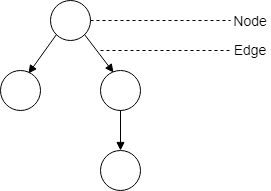
\includegraphics[width=0.33\textwidth]{Graph}
    \caption{Visuele representatie van een graaf}
    \label{fig:graph}
    \centering
\end{wrapfigure}

Game designers maken gebruik van de visual scripting interface die de editors bieden. Deze visual scripting interface bestaat uit visuele componenten die dienen als bouwblokken waaruit het verhaal is opgebouwd. Door deze bouwblokken op het canvas te plaatsen en met elkaar te verbinden kan er een verhaal worden geschreven. Zo zijn er bouwblokken waarmee conditionaliteit toegepast kan worden en bouwblokken die een content type vrij laten komen. Content typen zijn kleine datastructuurtjes met een betekenis in het verhaal. Een voorbeeld van zo’n content type is ‘text content’. Deze bevat een tekst die getoond zal worden in het spel. In \autoref{sec:contenttypen} zal er dieper worden ingegaan op content typen.

In de editors wordt een verhaal gerepresenteerd als een graph, in het Nederlands graaf genoemd\cite{Aho1983}. Een graaf bestaat uit nodes en edges, zoals weergeven in \autoref{fig:graph}. De nodes zijn de bouwblokken en de edges de verbindingen tussen deze bouwblokken. Aan de editors is het goed terug te zien dat het verhaal gerepresenteerd wordt als een graaf (\autoref{fig:storyeditorsimplegraph}).

In \autoref{ch:formalism} wordt er dieper ingegaan op het interpreteren van deze verhaal graaf. 

\begin{figure}[H]
    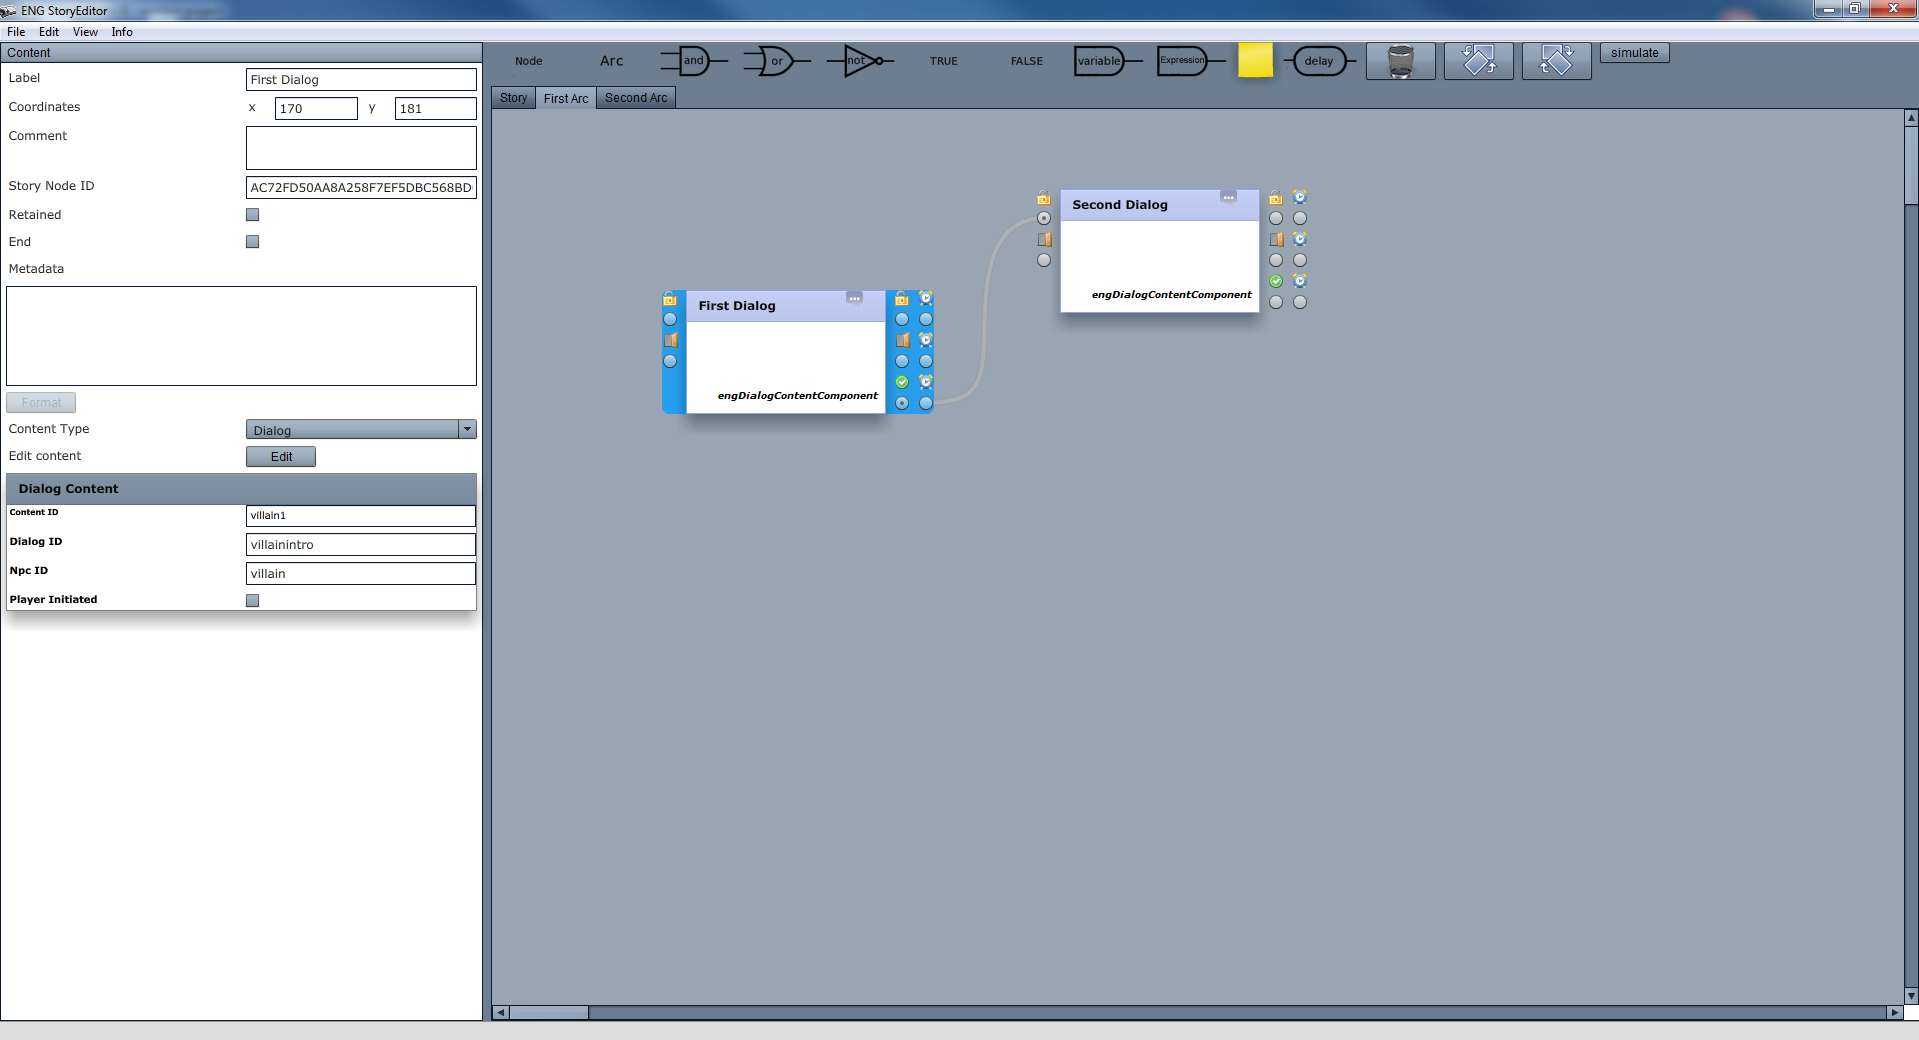
\includegraphics[width=\textwidth]{StoryEditor_SimpleStory_2dialogs}
    \caption{Een simpel verhaal gemaakt in de story editor}
    \label{fig:storyeditorsimplegraph}
    \centering
\end{figure}

\pagebreak

\section{Content typen}
\label{sec:contenttypen}
Iedere game bestaat uit game content. Dit is een verzamelnaam voor alle teksten, media en mechanieken die zich binnen het spel bevinden. Om onderscheid te maken tussen game content wordt er gebruik gemaakt van een bouwblok genaamd: content node. Deze bouwblokken bevatten een content type; een stukje game content. Denk hierbij aan een dialog, tekst of afbeelding. Ieder content type heeft een eigen betekenis en doel. In \autoref{fig:storyeditorsimplegraph} wordt er gebruik gemaakt van ‘dialog content’ welke een dialoog zal starten. Een ander voorbeeld van een content type is ‘text content’, deze kan als doel hebben om tekst te tonen. Verder bevatten content types ‘properties’. Dit zijn velden die verdere informatie geven over de eigenschappen van het doel. Zo heeft het content type ‘text content’ een property genaamd ‘Text' wat de tekst is die getoond zal worden door ‘text content’. Een content type is dus een datastructuur met een betekenis in de game. Door middel van content typen wordt er semantiek gebonden aan content nodes.

Door de semantische eigenschappen van een content node kunnen zowel de game designers als programmeurs onderscheid maken tussen game content. Programmeurs schrijven code om deze content types af te vangen en te interpreteren. Als er geen onderscheid bestaat weet de game engine niet wat er getoond moet worden wanneer er een content node vrijkomt.

Echter hebben de meeste content typen een vrij impliciet doel. Zo kan ‘text content’ een tekst bevatten die uitgesproken wordt door een karakter in het verhaal, maar het kan ook een mogelijk antwoord zijn dat de speler kan geven op een vraag. Om duidelijk onderscheid te maken is het belangrijk dat content typen zo expliciet mogelijk zijn in hun doel. Dit leidt naar content typen zoals ‘answer content’ en ‘quiz content’. Het is belangrijk dat er weinig ruimt is voor verschillende interpretaties.

\subsection{Vervuiling van de scope}
Een nadeel van content typen met een expliciet doel is dat ze meestal maar bruikbaar zijn voor een enkel project; de herbruikbaarheid van content typen is erg laag. Vooral in projecten waarin game content erg van elkaar verschild is dit een probleem. Per project worden er nieuwe content types aangemaakt, omdat de game content niet overeenkomt met vorige projecten. Echter kunnen al bestaande content typen niet worden verwijderd uit de editors, omdat de editor dan niet meer gebruikt kan worden voor oudere projecten. Dit alles zorgt voor een vervuiling van de content typen scope; content typen zijn beschikbaar in projecten die deze content niet benutten.

\pagebreak

\subsection{Statische definities}
\begin{wrapfigure}{r}{0.4\textwidth}
    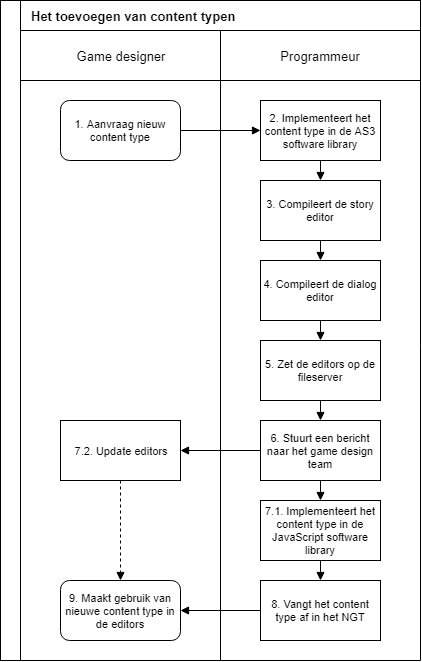
\includegraphics[width=0.38\textwidth]{Proces_ToevoegenContentTypeHuidig}
    \caption{Proces: het toevoegen van content types}
    \label{fig:procesaddcontenttypescurrent}
    \centering
\end{wrapfigure}
De editors maken gebruik van content types die gedefinieerd zijn in de \&ranj software library. In de software library bevinden zich klassen die ieder een content type vormen; content types hebben een statische definitie, ze zijn in de editor gebakken. Dit biedt wel meer controle over het content type, maar deze hoeveelheid controle overtollig, content types blijven datastructuren. Hiernaast maakt dit het proces van het toevoegen en verwijderen van content types lastiger. Om dit te bereiken moet de broncode van de editor worden aangepast en vervolgens moet de editor opnieuw worden gecompileerd. Het huidige proces voor het toevoegen van een content type ziet eruit als in \autoref{fig:procesaddcontenttypescurrent}.

\begin{enumerate}
    \item De game designer wilt onderscheid maken tussen quiz tekst die gebonden staat aan een tijdslimiet en vragen die de hoofdpersoon zichzelf stelt, waarbij de speler geen tijdsdruk heeft. De game designer heeft aparte content typen nodig om onderscheid te maken tussen deze twee typen game content.
    \item De programmeur implementeert deze content typen in de \&ranj ActionScript3 (AS3) software library. Uit deze library halen de editors de content types. In de software library wordt aan gegeven welke editors gebruik mogen maken van het content type. Hieruit kan geconcludeerd worden dat er geen encapsulatie van content typen bestaat. De editors zouden zelf aan moeten geven van welke content typen ze gebruik maken.
    \item De programmeur haalt de nieuwe versie van de AS3 library binnen en past het versie nummer aan. Hierna compileert de programmeur handmatig de story editor. Hierna wordt er “clone” achter de applicatie sleutel (application identifier) geplakt en de story editor voor de tweede keer gecompileerd. Dit maakt het openen van twee story editor schermen mogelijk. Anders kunnen er geen twee instanties van Apache Flex applicaties tegelijk openstaan.
    \item Stap 3 wordt herhaald door de programmeur, maar dan voor de dialog editor.
    \item De installers van de vier editors worden op de file server van \&ranj gezet. Dit is een gedeelde folder waar medewerkers van het bedrijf toegang tot hebben.
    \item De programmeur stuurt een mail naar het game design team waarin staat dat er een nieuwe versie van de editors beschikbaar is. Hiernaast staan veranderingen en de locatie van de nieuwe editor in de mail.
    \item Terwijl de game designers de editors updaten (7.2), implementeert de programmeur het content type in de JavaScript software library, zodat deze gebruikt kan worden in het 'narrative game template' (NGT).
    \item De programmeur vangt het nieuwe content type af in het NGT en linkt deze aan de correcte actie.
    \item De game designer kan gebruik maken van het nieuwe content type. De game interpreteert het content type.
\end{enumerate}

\noindent De programmeur moet eerst de Apache Flex editor projecten opgezet hebben en daarnaast kennis hebben van deze projecten. Hiernaast moet de editor handmatig getest worden na het toevoegen van de nieuwe content typen om te kijken of deze nog werkt.
Een geautomatiseerde deployment pipeline zou kunnen helpen en veel werk uithanden nemen van de programmeur. Hiernaast moet het compilatie en deployment proces zoveel mogelijk vermeden worden, omdat dit tijd kost. Content typen blijven datastructuurtjes en het toevoegen of aanpassen van deze structuren zou geen compilatie van beide editors moeten vereisen.

\subsection{Misbruik van content types}
Omdat het toevoegen of aanpassen van content typen een langdradig proces is wordt dit het liefst vermeden. Vaak worden er content typen uit oudere project misbruikt om onderscheid te kunnen maken tussen game content. Zo wordt ‘MinigameContent’ regelmatig gebruikt voor het tonen van hele andere dingen dan minigames.
Door content typen bij projecten op verschillende manieren te gebruiken kan er nooit op de eerste blik zeker gezegd worden wat voor doel het content type heeft.

\section{Dataschema’s}
Vanwege de diversiteit in game content verschillen de content typen sterk per project. De selectie aan content types wordt geacht om dynamisch te zijn. Deze staan echter statisch gedefinieerd in de \&ranj AS3 software library. Er moet een manier komen om per project een selectie aan content typen te kunnen specificeren.
Een content type is een (kleine) datastructuur die bestaat uit een aantal velden. Zo bestaat ‘sms content’, een content type die een SMS vrij laat komen, uit een afzender, datum en inhoud. Door in ActionScript3 een type aan een veld toe te kennen kan er worden afgedwongen dat afzender en inhoud een tekst zijn en dat de datum een datum is. Vervolgens verbiedt de user interface foutief gebruik; de datum moet in een correct formaat staan. Restricties opleggen aan de user interface als validatie is gevaarlijk, want het is nog steeds niet zeker of de data valide is omdat deze mogelijk ook op andere manier kan ontstaan. Er wordt dus gezocht naar een oplossing waarmee velden in een content type gespecificeerd kunnen worden. Hiernaast moeten deze velden gevalideerd kunnen worden.

\begin{wrapfigure}{r}{0.5\textwidth}
    \fbox{
        \parbox{0.48\textwidth}{
            \textbf{SMSContent} bestaat uit\\
            een \textbf{afzender} weergeven in \textbf{tekst}\\
            een \textbf{ontvang datum} weergeven als \textbf{datum}\\
            een \textbf{inhoud} weergeven als \textbf{tekst}
        }
    }
    \caption{Pseudo dataschema voor 'sms content'}
    \label{fig:pseudosmscontent}
\end{wrapfigure}

\pagebreak
\noindent Om de velden van de content typen te specificeren zal er gebruik gemaakt worden van dataschema’s. Met dataschema’s kan er een set aan regels worden opgelegd aan de datastructuur. Hierbij is het belangrijk dat het zowel leesbaar is voor mens als machine. Een pseudo dataschema voor ‘sms content’ zou eruit kunnen zien als in \autoref{fig:pseudosmscontent}.
Dit pseudo dataschema is leesbaar voor mensen, maar niet voor computers. Computers hebben een gestandaardiseerd formaat nodig om data te kunnen interpreteren, zoals Extensible Markup Language (XML) of JavaScript Object Notation (JSON).
Door gebruik te maken van een dataschema kan het proces voor het toevoegen van content typen sterk worden versimpeld. Het nieuwe proces wordt weergeven in \autoref{fig:procesaddcontenttypesnew}.

\begin{figure}[htb]
    \centering
    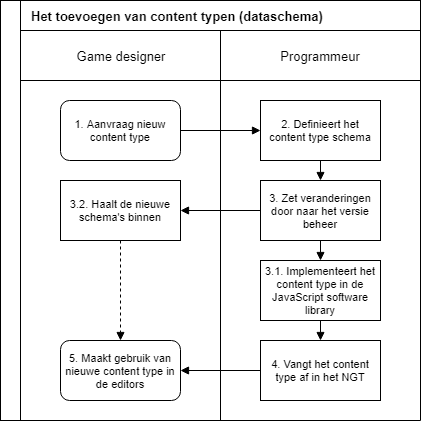
\includegraphics[width=0.72\textwidth]{Proces_ToevoegenContentTypeNieuw}
    \caption{Een versimpeld proces voor het toevoegen van content typen.}
    \label{fig:procesaddcontenttypesnew}
\end{figure}

\pagebreak
\subsection{XML-dataschema}
XML heeft dataschema functionaliteit; de onderliggende structuur van een XML-object kan worden gespecificeerd. Dit bereikt XML door middel van elementen en attributen. De eerder beschreven ‘sms content’ kan worden beschreven in een XML-dataschema als in \autoref{fig:xmlschemasmscontent}. Vervolgens kunnen XML-objecten gevalideerd worden door het schema. Het XML-object in \autoref{fig:xmlsmscontent} is valide, want de structuur komt overeen met die van het dataschema in \autoref{fig:xmlschemasmscontent}. JSON mist deze functionaliteit.

\begin{figure}[htb]
    \centering
    \lstset{
    language=XML,
    morekeywords={encoding,
        xs:schema,xs:element,xs:complexType,xs:sequence,xs:attribute}
    }
    \begin{lstlisting}
    <?xml version="1.0" encoding="UTF-8"?>
    <xs:schema xmlns:xs="http://www.w3.org/2001/XMLSchema">
        <xs:element name="smscontent">
            <xs:complexType>
                <xs:sequence>
                    <xs:element name="sender" type="xs:string" />
                    <xs:element name="receiveDate" type="xs:dateTime" />
                    <xs:element name="content" type="xs:string" />
                </xs:sequence>
            </xs:complexType>
        </xs:element>
    </xs:schema>                
    \end{lstlisting}
    \caption{XML-dataschema voor 'sms content'.}
    \label{fig:xmlschemasmscontent}
\end{figure}

\begin{figure}[htb]
    \centering
    \lstset{language=XML}
    \begin{lstlisting}[firstnumber=1]
    <?xml version="1.0" encoding="UTF-8"?>
    <smscontent>
        <sender>Harold</sender>
        <receiveDate>2018-04-21T11:00:00</receiveDate>
        <content>Great moves, keep it up!</content>
    </smscontent>              
    \end{lstlisting}
    \caption{Valide XML-object van 'sms content'.}
    \label{fig:xmlsmscontent}
\end{figure}

\pagebreak
\subsection{JSON-dataschema}
JSON is een populaire keuze; het is klein en snel. Er kwam steeds meer vraag naar nieuwe functionaliteiten, zoals het kunnen specificeren van schema’s\cite{Severance2012}. 
Vanwege de vraag naar schema’s in JSON is het er een woordenboek opgezet waarmee JSON-schema’s opgezet kunnen worden\cite{JsonSchemaOrg}. In dit woordenboek staan afspraken over keywords en hun functionaliteit. Door gebruik te maken van deze keywords, met name type en properties, kan het schema voor ‘sms content’ wordt opgezet zoals in \autoref{fig:jsonschemasmscontent}. Het JSON-document in \autoref{fig:jsonsmscontent} is valide volgens het schema in \autoref{fig:jsonschemasmscontent}.

\begin{figure}[htb]
    \centering
    \lstset{language=JSON}
    \begin{lstlisting}
    {
        "type": "object",
        "properties": {
            "sender": {
                "type": "string"
            },
            "date": {
                "type": "string",
                "format": "date-time"
            },
            "content": {
                "type": "string"
            }
        }
    }             
    \end{lstlisting}
    \caption{JSON-schema voor 'sms content'.}
    \label{fig:jsonschemasmscontent}
\end{figure}

\begin{figure}[htb]
    \centering
    \lstset{language=JSON}
    \begin{lstlisting}
    {
        "sender": "Harold",
        "date": "2018-04-21T11:00:00",
        "content": "Great moves, keep it up!"
    }                   
    \end{lstlisting}
    \caption{Valide JSON-document van 'sms content'.}
    \label{fig:jsonsmscontent}
\end{figure}

\pagebreak
\section{Een schaalbaar dataschema voor content types}
XML komt met out of the box dataschema functionaliteit, in JSON worden dataschema gemaakt op basis van afspraken. Echter zal er gebruik worden gemaakt van JSON-schema’s, omdat deze beter integreert met de nieuwe tech stack. JavaScript zelf komt direct met JSON ondersteuning wat het makkelijk maakt om deze om te zetten in objecten en uit te lezen. Verder blijkt uit benchmarking tests dat JSON lichter en sneller is dan XML\cite{Nurseitov}. 

\subsection{JSON-schema structuur}
Ieder JSON-schema beschikt over de volgende structuur:
\begin{itemize}
    \item \$schema; geeft aan dat een JSON-document een JSON-schema is. Hiernaast geeft de waarde aan welke schema versie dit schema voldoet\cite{Droettboom2016}. Dit kan ook een aangepast schema zijn die afwijkt van het originele schema, om bijvoorbeeld, uitgebreide functionaliteit te ondersteunen.
    \item \$id; Definieert een Uniform Resource Identifier (URI) voor het schema. Deze URI kan gebruikt worden om te refereren naar het bijbehorende schema.
    \item title; Titel van het schema
    \item description; Omschrijving van het schema; waar het schema voor staat.
    \item definitions; Optionele sectie waarin schema definities geplaatst kunnen worden die in het daadwerkelijke schema hergebruikt kunnen worden\cite{FoundationsJSONSchema}.
    \item Het daadwerkelijk schema waartegen JSON-documenten gevalideerd worden. Een voorbeeld is terug te zien in \autoref{fig:jsonschemasmscontent}.
\end{itemize}

\subsection{Referenties}
Om het schema schaalbaar op te zetten zullen mogelijke properties van content typen gedefinieerd worden onder ‘definitions’. Een voorbeeld hiervan is terug te zien in \autoref{fig:contenttypejsonschemaexample}. Deze properties kunnen vervolgens worden (her)gebruikt in de daadwerkelijke content typen, door gebruik van het \$ref keyword\cite{Droettboom2016}. Dit keyword refereert naar een ander schema via het schema \$id.

\begin{figure}[H]
    \centering
    \lstset{language=JSON}
    \begin{lstlisting}
    {
        "$schema": "http://json-schema.org/draft-07/schema#",
        "$id": "http://www.ranjnet.nl/content#",
        "definitions": {
            "propertyTypes": {
                "stringProperty": {
                    "$id": "#/definitions/propertyTypes/stringProperty",
                    "type": "string",
                    "default": ""
                }
            }
        }
    }                            
    \end{lstlisting}
    \caption{Voorbeeld content type JSON-Schema.}
    \label{fig:contenttypejsonschemaexample}
\end{figure}

\noindent Met deze properties kan er een basis content schema worden opgezet. Deze bevat properties die in elk concrete content type terugkomen. In \autoref{fig:basecontentjsonschema} staat een voorbeeld van een simpel base content schema die gebruik maakt van de eerder gedefinieerde string property.

\begin{figure}[htb]
    \centering
    \lstset{language=JSON}
    \begin{lstlisting}
    {
        "baseContent": {
            "type": "object",
            "properties": {
                "type": {
                    "$ref": "#/definitions/propertyTypes/stringProperty"
                }
            }
        }
    }               
    \end{lstlisting}
    \caption{JSON-schema van base content.}
    \label{fig:basecontentjsonschema}
\end{figure}

\subsection{Combinaties}
Door een ‘base content’ schema te definiëren met properties die voorkomen in ieder content type schema wordt de grootte van het JSON-schema minimaal gehouden. Hergebruikt van andere schema’s vergroot de schaalbaarheid van het schema.
Het ‘base content’ schema moet gecombineerd kunnen worden met de daadwerkelijke content types die gebruikt zullen worden in de editor en het NGT. Hiervoor maakt JSON-schema gebruik van het ‘allOf’ keyword. Een schema met het ‘allOf’ keyword is pas valide wanneer de onderliggende schema’s, gespecificeerd in ‘allOf’, valide zijn\cite{Droettboom2016}. Het schema in \autoref{fig:jsonschemaallofexample} definieert ‘text content’, welke valide is als de twee onderliggende schema’s valide zijn.
De ‘\$ref’ en ‘allOf’ keywords brengen complicaties met zich mee die in een later hoofdstuk besproken zullen worden.

\begin{figure}[htb]
    \centering
    \lstset{language=JSON}
    \begin{lstlisting}
    {
        "textContent": {
            "allOf": [
                {
                    "$ref": "#/definitions/baseContent"
                },
                {
                    "$id": "#/contentTypes/textContent",
                    "title": "Text content",
                    "description": "Textual content",
                    "properties": {
                        "text": {
                            "$ref": "#/definitions/propertyTypes/stringProperty"
                        }
                    }
                }
            ]
        }
    }
    \end{lstlisting}
    \caption{Een content schema die gebruik maakt van het 'allOf' keyword.}
    \label{fig:jsonschemaallofexample}
\end{figure}

\section{Het aanpassen van content type properties}
De properties van een content node kunnen worden aangepast door de gebruiker. Het selecteren van een content node resulteert in het tonen van de bijbehorende properties. De inspector (te zien in \autoref{fig:storyeditorinspector}) is verantwoordelijk voor het tonen van deze properties.

\begin{figure}[htb]
    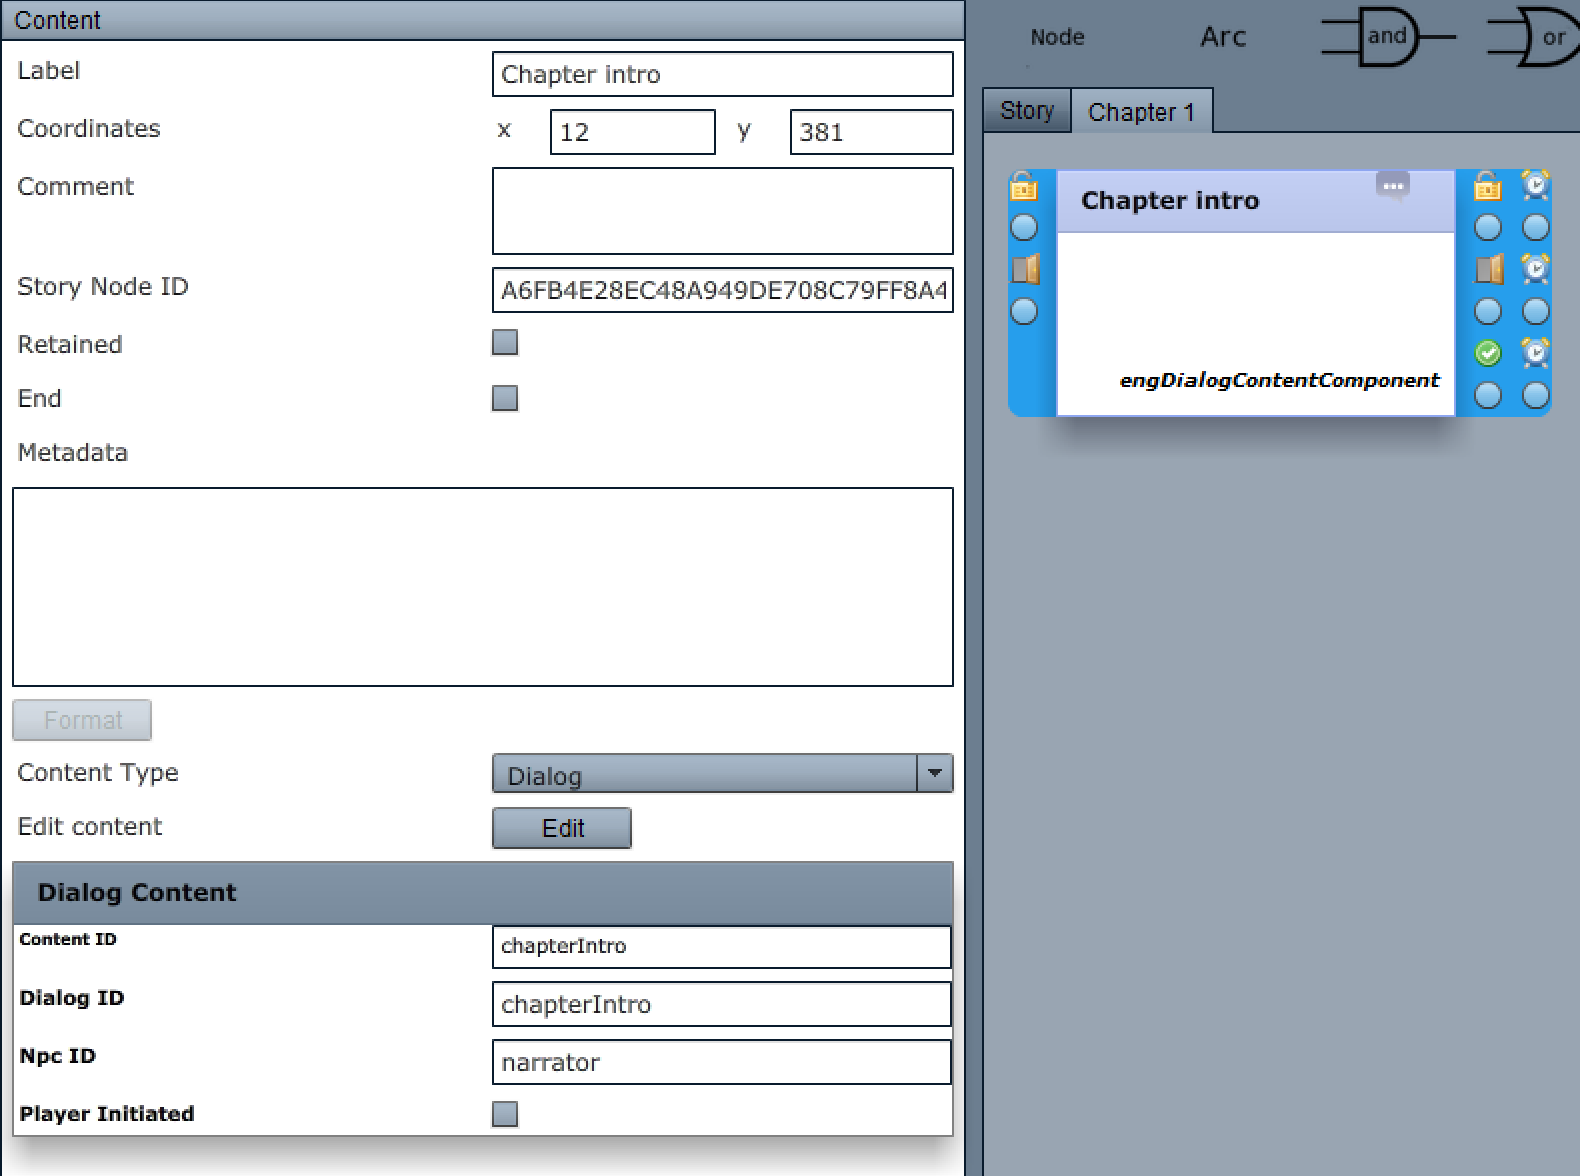
\includegraphics[width=\textwidth,height=\textheight,keepaspectratio]{StoryEditor_Inspector}
    \caption{De inspector die een geselecteerde dialog node toont.}
    \label{fig:storyeditorinspector}
    \centering
\end{figure}

In de nieuwe editor moet de inspector de properties tonen van het bijbehorende schema. Bij het opzetten van het content schema is er gebruik gemaakt van referenties om properties toe te kennen aan content typen. Dit resulteert in een schaalbaar JSON-schema, maar introduceert een probleem voor de inspector. Deze kan niet omgaan met referenties en combinaties van schema’s.

\subsection{Het content schema voorbereiden}
Om het content schema bruikbaar te maken voor de inspector moeten de volgende stappen worden ondernomen:

\begin{enumerate}
    \item Referenties resolven; ‘\$ref’ keywords vervangen door het daadwerkelijke gerefereerde object.
    \item Combinaties platslaan; ‘allOf’ keywords vervangen door een samenvoeging van onderliggende schema’s.
\end{enumerate}

Deze stappen moeten worden uitgevoerd wanneer de editor opstart, omdat het wenselijk is om deze functionaliteit te hebben bij het opzetten van het schema. De editor maakt dan een interne copy van het schema en zet deze om naar een schema zonder referenties en combinaties.

\subsubsection{Het oplossen van referenties}
Om referenties te resolven moet er eerst gekeken worden naar hoe het \$id keyword werkt. In de root, het hoogste niveau, van het JSON-schema wordt de locatie van het schema aangegeven. Het schema zelf dient toegankelijk te zijn op deze locatie om referenties vanuit andere schema’s toe te laten \cite{DraftJSONSchema07}. Binnen content type schema’s kan gebruik gemaakt worden van een hashtag (\#) om te refereren naar het root schema.

Als voorbeeld voor het resolven van referenties wordt er gekeken naar \autoref{fig:jsonschemrefexample}. Deze specificeert een schema voor ‘base content’ waarin gerefereerd wordt naar een ander schema, namelijk ‘string property’. Het pad van de referentie luidt: “\#/definitions/propertyTypes/stringProperty”. Hierin verwijst de hashtag naar de root van het schema: “http://www.ranjnet.nl/content”. Het bijbehorende object kan gevonden worden door vanaf de root te reduceren volgens het pad. Vervolgens wordt het \$ref keyword vervangen door het gevonden schema.
De community rondom JSON-schema leidt ook tot bestaande oplossingen zoals ‘json-schema-ref-parser’\footnote{https://github.com/BigstickCarpet/json-schema-ref-parser} en ‘json-schema-deref’\footnote{https://github.com/bojand/json-schema-deref }. Beide oplossingen zijn libraries die \$ref keywords resolven.


\begin{figure}[htb]
    \centering
    \lstset{language=JSON}
    \begin{lstlisting}
    {
        "$schema": "http://json-schema.org/draft-07/schema#",
        "$id": "http://www.ranjnet.nl/content#",
        "definitions": {
            "propertyTypes": {
                    "stringProperty": {
                    "$id": "#/definitions/propertyTypes/stringProperty",
                    "type": "string",
                    "default": ""
                }
            }
        },
        "baseContent": {
            "type": "object",
            "properties": {
                "type": {
                    "$ref": "#/definitions/propertyTypes/stringProperty"
                }
            }
        }
    }          
    \end{lstlisting}
    \caption{Een JSON-Schema met referentie.}
    \label{fig:jsonschemrefexample}
\end{figure}


\subsubsection{Het platslaan van combinaties}
Combinaties gemaakt door het ‘allOf’ keyword kunnen worden platgeslagen door de onderliggende schema’s samen te voegen in één schema object. Er wordt een object gemaakt waarnaar de velden van de onderliggende schema’s gekopieerd worden. Dit proces begint bij het eerste onderliggende schema wat betekent latere schema’s eventuele al bestaande velden zullen overschrijven.
Hoewel deze stap nodig is om het schema bruikbaar te maken voor de inspector is het samenvoegen van onderliggende schema’s niet juist volgens de definitie van het ‘allOf’ keyword. Volgens JSON-schema is een schema met ‘allOf’ pas valide wanneer elk onderliggend schema valide is\cite{FoundationsJSONSchema}. Dit betekent dat onderliggende schema’s niks van elkaar af weten. Door onderliggende schema’s plat te slaan naar één schema wordt deze barrière gebroken wat leidt tot een overtreding van JSON-schema.

\pagebreak
\subsection{Reflecteren van content types in de inspector}
De inspector moet het content type van een geselecteerde content node inzichtelijk en bewerkbaar maken. Bij ‘text content’ schema, die bestaat uit een string property, moet de inspector dan ook een tekstveld tonen waarmee de tekst in het content type kan worden aangepast.
\subsubsection{Primitieve types}
Omdat content types gedefinieerd zijn in JSON-schema’s, moet de inspector alle zes primitieve types\cite{Droettboom2016} ondersteunen om het schema te kunnen reflecteren. De selectie van primitieve types in JSON-schema bestaan uit:

\begin{enumerate}
    \item string
    \item boolean
    \item number
    \item object
    \item array
    \item null
\end{enumerate}

Ieder type heeft een eigen representatie. Met React kan de representatie van ieder type worden ingekapseld in componenten.

In \autoref{fig:representationschematypes} wordt een voorstel gedaan voor de representatie van de types\footnote{“null” heeft geen representatie}.

\subsubsection{Compositie}
Het voorstel in \autoref{fig:representationschematypes} maakt gebruik van een compositie structuur; types kunnen voorkomen in andere types. Zo komen de types ‘string’ en ‘number’ terug in het object type. Een compositie structuur bestaat uit een boom van ‘composites’ en ‘leaves’. Composite objecten bevatten andere composite- en leaf objecten (\autoref{fig:compositetree}), zo zijn de types ‘object’ en ‘array’ composities. Leaf objecten beheren geen onderliggende objecten. De boom is valide wanneer deze begint met een composite en eindigt met leaves.

\begin{figure}[H]
    \centering
    \begin{minipage}{.5\textwidth}
        \centering
        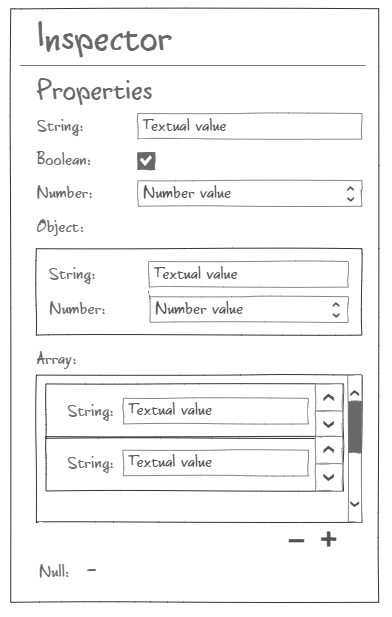
\includegraphics[width=.82\linewidth]{WireframeInspector}
        \caption{Representatie van primitieve JSON-schema types.}
        \label{fig:representationschematypes}    
    \end{minipage}%
    \begin{minipage}{.5\textwidth}
        \centering
        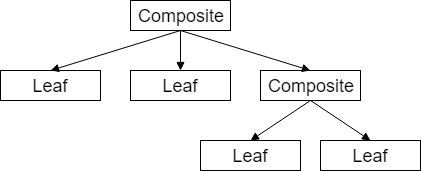
\includegraphics[width=.82\linewidth]{CompositeTree}
        \caption{Een valide compositie boom.}
        \label{fig:compositetree}
    \end{minipage}
\end{figure}

\pagebreak

\section{Conclusie}
Met deze conclusie wordt de deelvraag “Hoe kan diverse game content ondersteund worden?” beantwoord.

Diverse game content kan worden ondersteund door gebruik te maken van content typen. Het specificeren van content typen door middel van dataschema’s maakt het beheren van content typen mogelijk en draagt bij aan de flexibiliteit van de editors. JSON-schema is een licht en snel dataschema formaat geschreven in JSON. Door middel van referenties en combinaties kan er een schaalbaar dataschema worden opgezet. Omdat JavaScript JSON out-of-the-box ondersteunt is deze goed te integreren met de nieuwe technology stack die gebruik maakt van JavaScript. Hiernaast zijn er bestaande oplossingen in de vorm van libraries voor het valideren, manipuleren en reflecteren van JSON-schema’s.

\section{Vervolgonderzoek}
\paragraph{Vervuiling van de content typen selectie}
Om vervuiling van de content typen selectie te voorkomen zullen de JSON-schema’s deel uit gaan moeten maken van het project. Zo beschikt iedere game over een selectie aan content typen die voor haar relevant is. In de huidige situatie staan de editors los van de game engine. Om game content te kunnen bewerken die specifiek is voor een project zullen de editors opgenomen moeten worden in een overkoepelde projectstructuur.

\paragraph{JSON-schema combinatie keywords}
Met deze oplossing kan er geen gebruik gemaakt worden van andere combinatie keywords die JSON-schema biedt. Naast het ‘allOf’ keyword zijn er ook nog de combinatie keywords: ‘anyOf’, ‘oneOf’ en ‘not’.


\chapter{Formalismen}
\label{ch:formalism}
In dit hoofdstuk wordt er gekeken naar formalisme binnen interactive story telling. Er wordt een voorstel gedaan op de softwarearchitectuur van de nieuwe editor om meerdere formalisme te ondersteunen in één omgeving. Deze softwarearchitectuur betreft het leggen van een scheiding tussen de editor en het achterliggende formalisme. Het ondersteunen van meerdere formalismen maakt het onderhouden van twee aparte editors overbodig.

\section{Formalismen binnen interactive story telling}
\subsection{De rol van formalisme}
Het formaliseren van het narratief speelt een grote rol tijdens het ontwikkelproces van narrative games. Volgens een vastgesteld formalisme wordt er betekenis gegeven aan de structuur achter het narratief. Een formalisme is een theorie die bepaalde richtlijnen afdwingt en waarde koppelt aan syntax. In \autoref{fig:simplestorytree} is een voorbeeld van een formalisme terug te zien. Dit formalisme wordt ook wel een story graph genoemd.

Een formalisme dient als een communicatiemiddel tussen zowel mens als computer. Mensen en computers die kennis hebben van het formalisme interpreteren deze vrijwel hetzelfde. Hierdoor kunnen teamleden efficiënt samenwerken aan een narratief; ze zitten op dezelfde lijn en structureren beide volgens het formalisme.

\subsection{Formalismen voor verschillende doeleinden}
\subsubsection{Story graphs}

\begin{wrapfigure}{r}{0.4\textwidth}
    \centering
    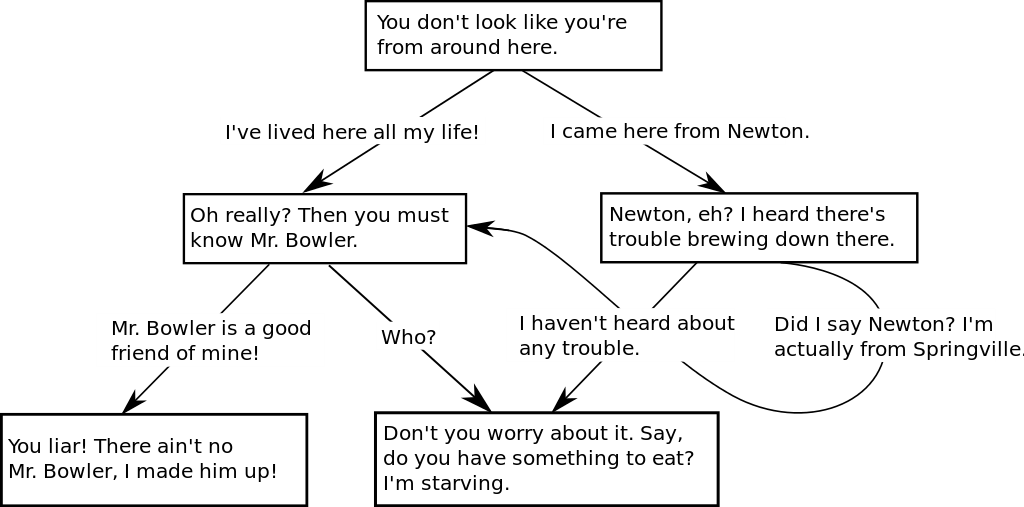
\includegraphics[width=0.38\textwidth]{SimpleStoryTree}
    \caption[]{Een simpele story tree. \footnotemark}
    \label{fig:simplestorytree}
\end{wrapfigure}
\footnotetext{Bron: \url{https://commons.wikimedia.org/wiki/File:Dialog_tree_example.svg}}


Veel interactieve verhalen met vertakkingen kunnen worden gerepresenteerd als een boom\cite{GalyeanIII1995}. Deze bestaat uit nodes (ook wel vertices genoemd) die de uiting van de gesprekspartner representeren. Na de evaluatie van deze nodes kan er een keuze gemaakt worden. Deze discrete set van keuzes zijn terug te zien in de story tree als edges, hetgeen dat de nodes met elkaar verbindt. De gemaakte keuze bepaald de volgende node die geëvalueerd zal worden en dus de uitkomst van het verhaal. Dit formalisme laat ons toe om een inzichtelijk en simpele dialoog tussen twee personen te modelleren (\autoref{fig:simplestorytree}).

\subsubsection{Behaviour tree}
// todo

\pagebreak
\subsection{Syntactische vormen}

\begin{wrapfigure}{r}{0.4\textwidth}
    \centering    
    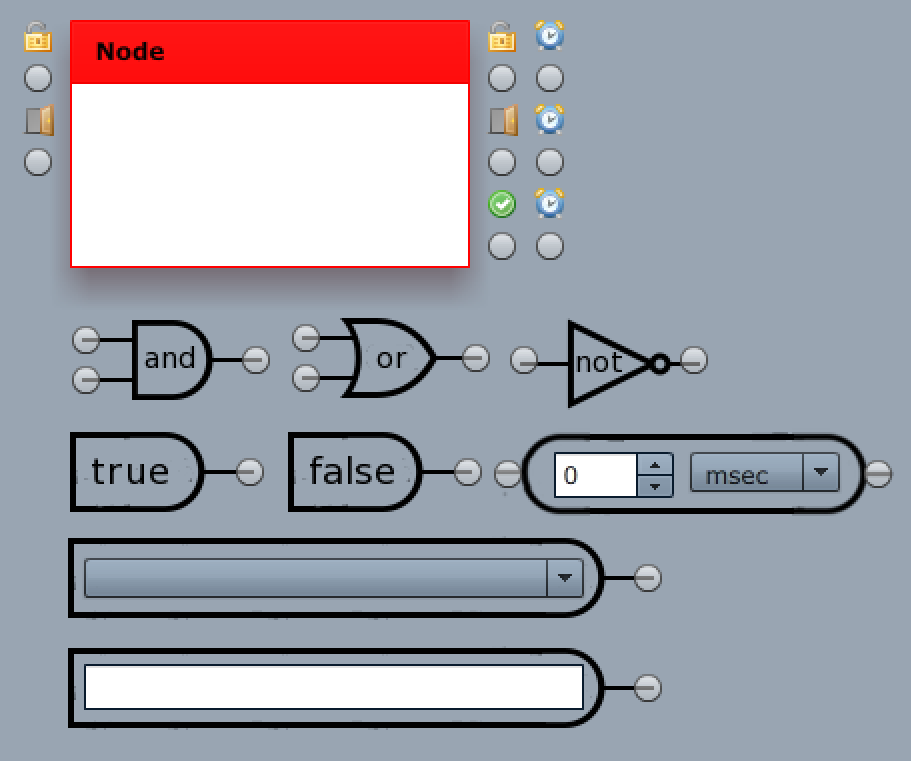
\includegraphics[width=0.38\textwidth]{SyntactischeVormen}
    \caption{Bouwblokken in de story editor.}
    \label{fig:syntactischevormen}
\end{wrapfigure}

Volgens formalisme kan een narratief uitgedrukt worden in syntactische vormen. Deze hebben verder geen waarde of betekenis, totdat er een interpretatie op losgelaten wordt. Een goed voorbeeld hiervan is terug te zien in de wiskunde. 

Zo bestaat de stelling van Pythagoras ook uit syntactische vormen die weergeven worden als letters:

\[ a^2 + b^2 = c^2 \]

Binnen de wiskunde hebben deze letters volgens het formalisme zelf geen betekenis. Dit wordt onderbouwd door het feit dat letters gebruikt kunnen worden voor andere stellingen, functies en vergelijkingen. De interpretatie op de eigenschappen van letter, zoals positie binnen de stelling, geven betekenis aan deze syntactische vorm.

Dit begrip komt ook terug in de editors in de vorm van nodes. Met deze nodes wordt er een narratief geformuleerd die de richtlijnen van het formalisme respecteert. We kunnen ook wel zeggen dat deze syntactische vormen bouwblokken zijn in de editors. In \autoref{fig:syntactischevormen} zijn enkele bouwblokken die in de story editor voorkomen te zien.

\section{Formalisme binnen de story- en dialog editor}
De story- en dialog editor maken beide gebuikt van een ander formalisme. Dit is duidelijk te zien aan hoe het narratief representeert wordt door de editors (zie \autoref{fig:storyeditorvisualisationofstorydata} en \autoref{fig:dialogeditorvisualisationofstorydata}). 

% \begin{figure}
%     \centering
%     \begin{minipage}{.45\textwidth}
%         \centering
%         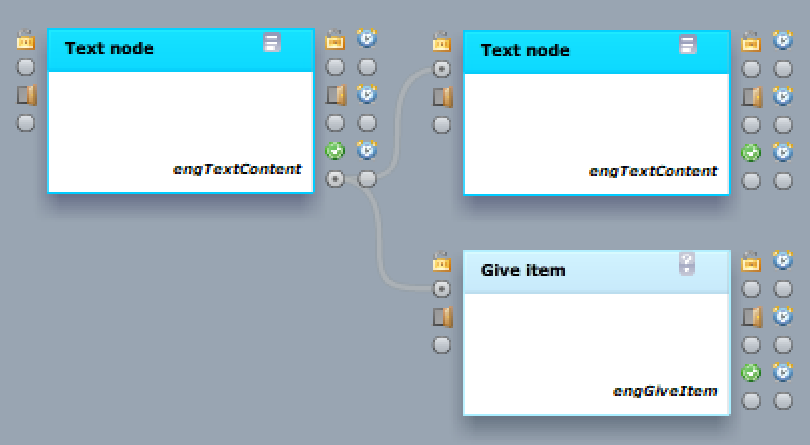
\includegraphics[height=0.4\linewidth]{StoryEditorVisualisationOfStoryData}
%         \caption{Story editor visualisatie van achterliggende data.}
%         \label{fig:storyeditorvisualisationofstorydata}
%     \end{minipage}%
%     \begin{minipage}{.45\textwidth}
%         \centering
%         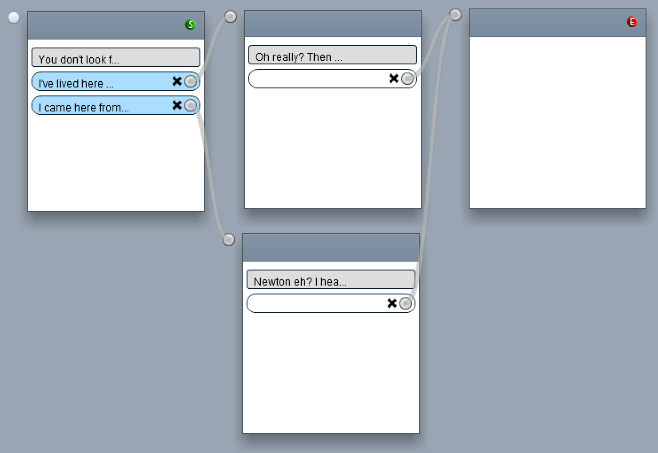
\includegraphics[height=0.4\linewidth]{DialogEditorVisualisationOfStoryData}
%         \caption{Dialog editor visualisatie van achterliggende data.}
%         \label{fig:dialogeditorvisualisationofstorydata}
%     \end{minipage}
% \end{figure}

\begin{figure}[htb]
    \centering
    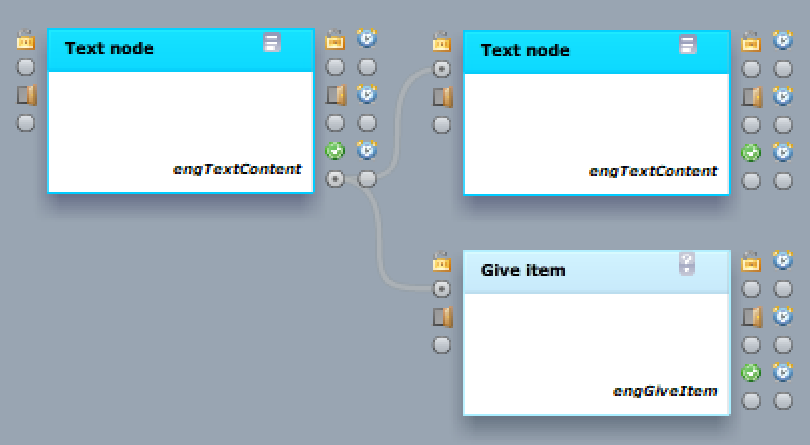
\includegraphics[width=0.45\textwidth]{StoryEditorVisualisationOfStoryData}
    \caption{Story editor visualisatie van achterliggende data.}
    \label{fig:storyeditorvisualisationofstorydata}
\end{figure}

\begin{figure}[htb]
    \centering
    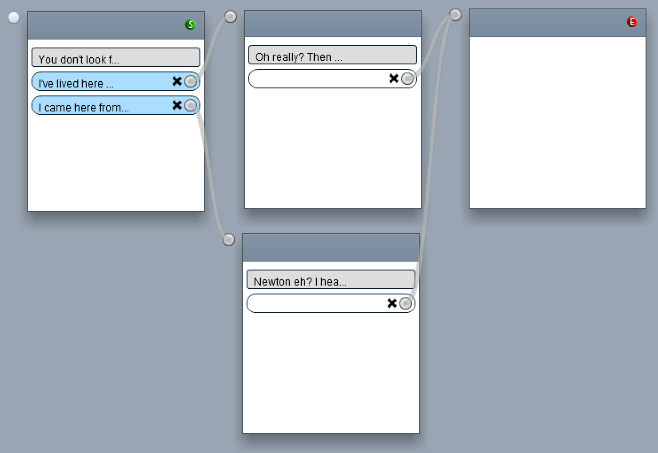
\includegraphics[width=0.45\textwidth]{DialogEditorVisualisationOfStoryData}
    \caption{Dialog editor visualisatie van achterliggende data.}
    \label{fig:dialogeditorvisualisationofstorydata}
\end{figure}

Aan de huidige code base is te zien dat er een nauwe koppeling bestaat tussen de interface en het achterliggende formalisme. Dit maakt het lastig om meerdere formalismen te ondersteunen.

Dit kan een reden zijn geweest waarom er twee editors zijn opgezet; om de scheiding te maken tussen formalismen. Het is een uitdaging om in één omgeving meerdere formalismen te ondersteunen, omdat deze bestaat uit andere syntactische vormen en gebruik maken van andere principes.

Wel is het wenselijk om meerdere formalismen in één omgeving te ondersteunen om de volgende voorkomende problemen op te kunnen lossen:

\begin{itemize}
    \item Houdbaarheid; er hoeft nog maar één omgeving onderhouden te worden in plaats van twee wat schilt in kosten.
    \item Houdbaarheid; generieke editor functionaliteit (copy/ paste, verplaatsen van nodes) kan worden hergebruikt en hoeft maar één keer geïmplementeerd te worden.
    \item Future proofing; benodigde formalismen kunnen in de toekomst worden toegevoegd. Er hoeft niet nog een nieuwe editor gemaakt te worden.
    \item Co-creatie; er zou eventueel een versimpeld formalisme toegevoegd kunnen worden waar klanten mee overweg kunnen. Hiernaast kan het versimpelde formalisme gebruikt worden om de volledige flow van het verhaal in kaart te brengen. Bij \&ranj is er al onderzoek gedaan naar formalisme voor klant co-creatie \cite{Schipper2015}.
\end{itemize}

\section{De scheiding leggen tussen de editor en formalisme}
Om een flexibele tool op te zetten voor het vertellen van diverse digitale interactieve verhalen is het nodig om verschillende formalisme voor diverse doeleinden te kunnen gebruiken. Met de toekomst blik van \&ranj en het ‘bad news’ dialoog moet er een formalisme ondersteund worden waarin een meer AI-benadering toegepast kan worden. Om dit mogelijk te maken moet er een manier komen om formalismen toe te kunnen voegen aan de editors.

Om de scheiding te leggen tussen de editor en het achter liggende formalisme zijn de volgende vragen opgesteld:

\begin{itemize}
    \item Hoe kunnen er bouwblokken worden geformuleerd per formalisme?
    \item Hoe kunnen er regels worden opgelegd aan het verbinden en het in elkaar voegen van deze bouwblokken?
    \item Hoe zou een algoritme eruitzien om vanuit een visuele structuur te compileren naar een formalisme?
\end{itemize}

\subsection{Het formuleren van bouwblokken}
\label{subsec:formulerenvanbouwblokken}
Ieder formalisme wordt ondersteund door syntactische vormen. Een concretere naam die aansluit bij de editors hiervoor is ‘bouwblokken’. Gebruikers van de editors zullen deze bouwblokken gebruiken om een narratief te definiëren volgens een vooraf vastgesteld formalisme. De representatie en interpretatie van deze bouwblokken verschillen dan ook per formalisme. Maar voor de editors zijn het allemaal ‘nodes’ (met eventuele porten) waarmee de node verbonden kan worden aan andere nodes; voor de editor hebben deze nodes geen verdere waarde noch betekenis. Als programmeur moet het mogelijk zijn om op een makkelijke manier bouwblokken te kunnen formuleren. Voor deze use case zijn de volgende requirements opgesteld:

\begin{enumerate}
    \item Ieder formalisme moet onderbouwd worden door een set aan bouwblokken, zodat de gebruiker deze kan gebruiken om binnen de richtlijnen van het formalisme te werken.
    \item Het constructie proces van de bouwblokken moet losstaan van de representatie, zodat verschillende representaties gebruikt kunnen worden voor diverse doeleinden.
    \item De representatie van deze bouwblokken moeten losgekoppeld worden van enige waarde of betekenis, zodat deze later volgens het formalisme geïnterpreteerd kunnen worden.
\end{enumerate}

\noindent De voornaamste manier om een node te construeren is om de bijbehorende klasse te instantiëren. Dit geeft ons een node object waarvan de representatie statisch is; het instantiëren van de node klassen resulteert altijd in hetzelfde object. Dit schendt requirements 2 en 3. Om constructie van representatie los te koppelen, en zo te voldoen aan de tweede requirement, kunnen er parameters de constructor van de node klasse gedefinieerd worden die de eigenschappen en representatie van de node beschrijven. In \autoref{fig:storyeditorvisualisationofstorydata} is een van de bouwblokken in het formalisme van de story editor terug te zien: de ContentTypeNode. Dit bouwblok heeft een label en 8 porten. Het zojuist beschreven constructie proces voor deze node zou er als volgt uit kunnen zien:\\


% listings cannot be used inside a frame box ;c
% \noindent\fbox{
%     \parbox{\textwidth}{
        \textbf{Functie handtekening}
        \lstset{language=JavaScript,breaklines=true}
        \begin{lstlisting}
            constructor Node(label: string, markup: string, allowBodyConnections: boolean, ports: Port[]): Node
        \end{lstlisting}

        \textbf{Voorbeeld}
        \lstset{language=JavaScript,breaklines=true}
        \begin{lstlisting}
            new Node('ContentType', '<rect class="node-body" width="100" height="100"><text/></rect>', false, [new Port(...), new Port(...), ...);
        \end{lstlisting}
%     }
% }

\noindent Deze manier van construeren heeft de volgende consequenties:
\begin{itemize}
    \item Een node moet geconstrueerd worden met argumenten die voldoen aan de parameters van de constructor. 
    \item Om achter de betekenis van de argumenten te komen moet er gekeken worden naar de constructor handtekening; argumenten zijn niet expliciet.
    \item Het stimuleert een nauwe koppeling tussen de node klasse en de achterliggende ‘diagramming library’ die de nodes visualiseert.
    \item Het stimuleert het aanroepen van het constructie proces op diverse plekken in de code.
    \item Er kunnen nodes worden gemaakt met verschillende representaties, door verschillende argumenten mee te geven.
\end{itemize}

\noindent Deze manier van construeren wordt al gauw ingewikkeld en onduidelijk ondervonden. Vooral omdat het constructie proces niet leesbaar en expliciet genoeg is. Daarnaast zal het constructie proces op verschillende plekken plaatsvinden, omdat er geen klasse bestaat die hier verantwoordelijk voor is. Dit heeft een grote invloed op de houdbaarheid van het product. Als er later een aanpassing aan een bouwblok gedaan moet worden zal dit relatief veel werk kosten en mogelijk fouten introduceren. Het constructie proces moet geabstraheerd worden, zodat het system onafhankelijk is van hoe de node objecten geïnstantieerd en gerepresenteerd worden. Door gebruikt te maken van ‘Creational design patterns’ kan er een abstractie laag worden geplaatst waardoor de gezochte scheiding kan worden gelegd\cite{DesignPatterns}.

Er is een kleine selectie aan patronen opgesteld die in aanmerking komen om het eerder beschreven probleem op te lossen. Deze design patterns zullen naast het probleem gelegd worden om de toepasselijkheid en consequenties in kaart te brengen. Uiteindelijk zal er een conclusie getrokken worden waarin het best passende design pattern ter sprake komt. De selectie aan design patterns die besproken zal worden bestaat uit:

\begin{itemize}
    \item Abstract factory
    \item Builder
    % \item Prototype
\end{itemize}

%% ABSTRACT FACTORY %%

\subsubsection{Abstract factory}
\noindent\textbf{Intentie}\\
De intentie van dit patroon wordt beschreven als volgt\cite{DesignPatterns}\cite{SourceMakingAbstractFactory}:
\begin{quote} 
    \centering    
    \textit{
        "Provide an interface for creating families of related or depent objects without specifying their concrete classes."       
    }
\end{quote}

\noindent\textbf{Toepasselijkheid}\\
Dit patroon helpt de editor onafhankelijk zijn van de manier waarop de nodes geconstrueerd en gerepresenteerd worden \cite{DesignPatterns}, wat inhaakt op een deel van de tweede requirement. Verder is het wenselijk om meerdere formalismen te ondersteunen. Hierbij spelen bouwblokken een grote rol: deze ondersteunen het gebruik van een formalisme binnen de editor. Volgens de eerste requirement moet de editor een set aan bouwblokken kunnen aanbieden die de gebruiker kan gebruiken. Het abstract factory patroon maakt het mogelijk om families van nodes te creëren \cite{DesignPatterns}. Hierbij is de familie het formalisme.
\newline

\noindent\textbf{Structuur}

\begin{figure}[H]
    \centering    
    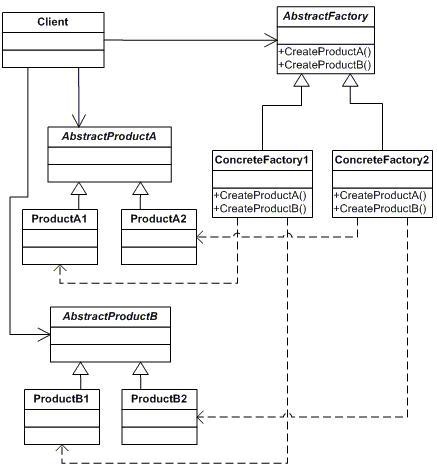
\includegraphics[width=0.55\textwidth]{AbstractFactoryUML}
    \caption[]{Klasse diagram van het abstract factory pattern. \footnotemark}
    \label{fig:abstractfactoryuml}
\end{figure}
\footnotetext{Bron: \url{http://www.dofactory.com/net/abstract-factory-design-pattern}}

\noindent\textbf{Deelnemers}
\begin{itemize}
    \item \textbf{AbstractFactory} (NodeFactory)
    \begin{itemize}
        \item Biedt een interface aan met methodes voor het maken van node objecten.
    \end{itemize}

    \item \textbf{ConcreteFactory} (StateMachineNodeFactory, BehaviourTreeNodeFactory)
    \begin{itemize}
        \item Implementeert de ‘NodeFactory’ om concrete node objecten te kunnen maken.
    \end{itemize}

    \item \textbf{AbstractProduct} (Node, mogelijke extra abstractie laag: StateMachineNode, BTNode ...)
    \begin{itemize}
        \item Biedt de interface voor een type van concrete node objecten.
    \end{itemize}
    \item \textbf{ConcreteProduct} (ContentNode, SelectorNode, ...)
    \begin{itemize}
        \item Implementeert ‘Node’ en maakt onderscheid tussen verschillende type nodes mogelijk.
        \item Definieert een product dat gemaakt zal worden door het desbetreffende concrete factory object.
    \end{itemize}
    \item \textbf{Client}
    \begin{itemize}
        \item Gebruikt de interfaces die gedefinieerd zijn door de ‘AbstractFactory’ en de ‘AbstractProduct’ klassen.
    \end{itemize}
\end{itemize}

\noindent\textbf{Consequenties}
\begin{itemize}
    \item Het isoleert de concrete node klassen; de factory heeft de verantwoordelijkheid en het proces om nieuwe nodes te maken.
    \item Het maakt het verwisselen van verschillende formalisme makkelijk; Elk formalisme zou een eigen factory kunnen hebben. De factory wordt op één plek in de code geïnstantieerd en omdat de concrete factories allemaal dezelfde interface implementeren kunnen we makkelijk van concrete factory verwisselen.
    \item Het dwingt het implementeren van interface af; elke concrete node zal de node interface moeten implementeren. Om subklasse specifieke operaties aan te kunnen roepen zal er gebruik gemaakt moeten worden van casting.
    \item Nieuwe nodes toevoegen is lastig; per type node zal er een methode bijkomen in zowel de abstract factory als de concrete factories. Hiernaast kan dit zorgen voor concrete factories die operaties bevatten met een lege body, omdat bepaalde type nodes niet van toepassing zijn in het formalisme dat de concrete factory ondersteund.
\end{itemize}

\noindent\textbf{Conclusie}\\
Het is wenselijk om het constructie proces te isoleren en te scheiden van de rest van de applicatie. Dit maakt het makkelijker om later eventueel van diagramming library te wisselen en nodes aan te passen. Verschillende implementaties van ‘AbstractFactory’ kunnen ieder nodes voor een formalisme aanbieden. Echter omdat elke ‘ConcreteFactory’ de ‘AbstractFactory’ implementeert zullen deze moeten voldoen aan de interface van de geabstraheerde factory. Dit kan zorgen voor lege methodes die verder geen waarde hebben. Hiernaast kan dit de illusie wekken dat elke node terugkomt in ieder formalisme. Tenslotte is het toevoegen van nieuwe nodes lastig. Volgens requirement 1 moet er een set aan bouwblokken aangeboden worden. Als er een nieuwe bouwblokken in de vorm van nodes aan de set toegevoegd moeten worden zal de interface van de ‘AbstractFactory’ ook aangepast moeten worden. Dit heeft als gevolg dat iedere ‘ConcreteFactory’ deze nieuwe methode ook moet implementeren. Hoe meer formalismen er zijn, des te moeilijker het zal zijn om nieuwe bouwblokken toe te voegen. Dit maakt het ‘Abstract Factory’ design pattern ongeschikt voor deze use case.

%% BUILDER %%
\subsubsection{Builder}
\noindent\textbf{Intentie}\\
De intentie van dit patroon wordt beschreven als volgt\cite{DesignPatterns}\cite{SourceMakingBuilder}:
\begin{quote} 
    \centering    
    \textit{
        "Separate the construction of a complex object from its representation so that the same construction process can create different representations."        
    }
\end{quote}

\noindent\textbf{Toepasselijkheid}\\
Het builder patroon is interessant omdat nodes een vrij complex object zijn die meerdere representaties zal hebben in de editor. Er moeten verschillende bouwblokken ondersteund worden (requirement 1) die ieder een eigen presentatie hebben (requirement 2). Hiernaast maakt het patroon het constructie proces expliciet door een interface aan te bieden waarmee nodes opgebouwd kunnen worden.
\newline

\noindent\textbf{Structuur}

\begin{figure}[H]
    \centering    
    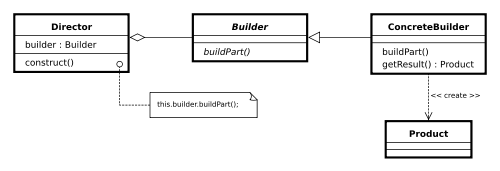
\includegraphics[width=0.7\textwidth]{BuilderUML}
    \caption[]{Klasse diagram van het builder pattern. \footnotemark}
    \label{fig:builderyuml}
\end{figure}
\footnotetext{Bron: \url{https://en.wikipedia.org/wiki/Builder_pattern}}

\noindent\textbf{Deelnemers}
\begin{itemize}
    \item \textbf{Builder} (NodeBuilder)
    \begin{itemize}
        \item Biedt een interface voor het maken van node onderdelen (e.g. porten, labels, visuals).
    \end{itemize}

    \item \textbf{ConcreteBuilder} (StateMachineNodeBuilder, BehaviourTreeNodeBuilder)
    \begin{itemize}
        \item Implementeert de ‘Builder’ interface en maakt het mogelijk om onderdelen te maken.
        \item Definieert en houdt bij hoe de representatie gemaakt wordt. 
        \item Biedt een interface om de uiteindelijke node te verkrijgen.

    \end{itemize}

    \item \textbf{Director} (StateMachineDirector, BehaviourTreeDirector)
    \begin{itemize}
        \item Gebruikt de ‘Builder’ interface om de verschillende bouwblokken per formalisme te construeren.
    \end{itemize}
    \item \textbf{Product} (ContentNode, SelectorNode, ...)
    \begin{itemize}
        \item Representeert de node waaraan de ‘ConcreteBuilder’ bouwt.
        \item Bevat de aangebouwde onderdelen en achterliggende model (e.g. content type of een expressie).
    \end{itemize}
\end{itemize}

\noindent\textbf{Consequenties}
\begin{itemize}
    \item Het isoleert het constructie proces en de representatie van nodes; de node editor hoeft niet te weten hoe een node gemaakt en gerepresenteerd wordt. De builder biedt een interface voor het construeren van nodes die de concrete builder implementeert. Deze code om nodes te creëren hoeft maar één keer geschreven te worden. Directors kunnen deze interface gebruiken om verschillende varianten van nodes te maken.
    \item Het constructie proces van nodes is explicieter; de builder biedt een interface met methodes die direct beschrijven welk onderdeel er gemaakt wordt. Zo is de constructie die plaats vindt in \autoref{fig:builderconstruction} explicieter dan \autoref{fig:constructionbyconstructor}.
    \item Fijnere controle over constructie proces van nodes; nodes worden stap voor stap in elkaar gezet. In tegenstelling tot andere creational design patterns worden nodes niet in één keer gemaakt.
\end{itemize}

\begin{figure}[htb]
    \centering
    \lstset{language=JavaScript}
    \begin{lstlisting}
        return this._builder
            .build<ContentNode>()
            .label('ContentNode')
            .addPort(CompletedPort)
            .addPort(UnlockedPort)
            .getNode();
    \end{lstlisting}
    \caption{Constructie stap voor stap door de 'Director', geschreven in TypeScript.}
    \label{fig:builderconstruction}
\end{figure}

\begin{figure}[htb]
    \centering
    \lstset{language=JavaScript}
    \begin{lstlisting}
        return new Node('ContentNode', [new Port(...)]);
    \end{lstlisting}
    \caption{Directe instantiatie door constructor.}
    \label{fig:constructionbyconstructor}
\end{figure}

\noindent\textbf{Conclusie}\\
Het builder patroon biedt de mogelijkheid om nodes stapsgewijs te construeren. Door middel van de interface die de ‘NodeBuilder’ klasse biedt kunnen nodes expliciet en modulair opgebouwd worden (zie \autoref{fig:builderconstruction}). Dit maakt het makkelijk om nieuwe bouwblokken te definiëren, zonder iets af te weten van hoe de nodes gemaakt worden. Deze code is één keer geschreven en bevind zich in de concrete builders. De ‘Director’ klasse kan geabstraheerd worden die per formalisme geïmplementeerd kan worden. Deze concrete directors kunnen een set aan bouwblokken opbouwen die makkelijk aan te passen is, waarmee voldaan wordt aan de eerste requirement. Het patroon biedt ook een fijnere controle over het constructie proces, omdat nodes stapsgewijs op gebouwd kunnen worden. Dit maakt het makkelijk om bouwblokken met verschillende representaties te creëren en hiermee wordt voldaan aan de tweede requirement.

%% PROTOTYPE %%
% \subsubsection{Prototype}
% \noindent\textbf{Intentie}\\
% De intentie van dit patroon wordt beschreven als volgt\cite{DesignPatterns}\cite{SourceMakingAbstractFactory}:
% \begin{quote} 
%     \centering    
%     \textit{
               
%     }
% \end{quote}

% \noindent\textbf{Toepasselijkheid}\\

% \newline

% \noindent\textbf{Structuur}

% \begin{figure}[H]
%     \centering    
%     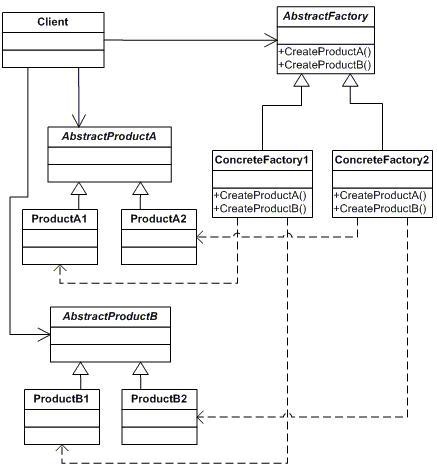
\includegraphics[width=0.8\textwidth]{AbstractFactoryUML}
%     \caption[]{Klasse diagram van het abstract factory pattern. \footnotemark}
%     \label{fig:abstractfactoryuml}
% \end{figure}
% \footnotetext{Bron: \url{http://www.dofactory.com/net/abstract-factory-design-pattern}}

% \noindent\textbf{Deelnemers}
% \begin{itemize}
%     \item \textbf{AbstractFactory} (NodeFactory)
%     \begin{itemize}
%         \item Biedt een interface aan met methodes voor het maken van node objecten.
%     \end{itemize}

%     \item \textbf{ConcreteFactory} (StateMachineNodeFactory, BehaviourTreeNodeFactory)
%     \begin{itemize}
%         \item Implementeert de ‘NodeFactory’ om concrete node objecten te kunnen maken.
%     \end{itemize}

%     \item \textbf{AbstractProduct} (Node, mogelijke extra abstractie laag: StateMachineNode, BTNode ...)
%     \begin{itemize}
%         \item Biedt de interface voor een type van concrete node objecten.
%     \end{itemize}
%     \item \textbf{ConcreteProduct} (ContentNode, SelectorNode, ...)
%     \begin{itemize}
%         \item Implementeert ‘Node’ en maakt onderscheid tussen verschillende type nodes mogelijk.
%         \item Definieert een product dat gemaakt zal worden door het desbetreffende concrete factory object.
%     \end{itemize}
%     \item \textbf{Client}
%     \begin{itemize}
%         \item Gebruikt de interfaces die gedefinieerd zijn door de ‘AbstractFactory’ en de ‘AbstractProduct’ klassen.
%     \end{itemize}
% \end{itemize}

% \noindent\textbf{Consequenties}
% \begin{itemize}
    
% \end{itemize}

% \noindent\textbf{Conclusie}\\

%\subsubsection{Conclusie}
% todo ...

% \subsubsection{Porten aan bouwblokken}

% \begin{wrapfigure}{r}{0.4\textwidth}
%     \centering    
%     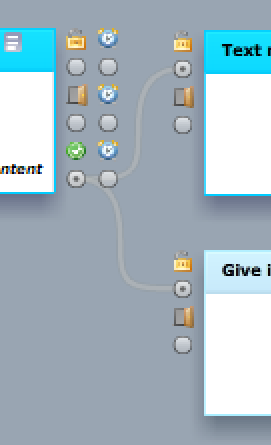
\includegraphics[width=0.38\textwidth]{StoryEditor_LinksBetweenNodes}
%     \caption{Verbonden porten in de huidige story editor.}
%     \label{fig:linksinstoryeditor}
% \end{wrapfigure}

% Formalismen kunnen gebruik van maken porten om relaties te leggen tussen bouwblokken, een voorbeeld hiervan is de huidige story editor (zie \autoref{fig:linksinstoryeditor}). Deze porten bevinden zich op een bepaalde positie relatief aan een bouwblok, voornamelijk: boven, onder, links of rechts. Hiernaast zullen er zeldzame gevallen voorkomen waarbij porten op een andere positie zullen staan.

% In de huidige editors lijken de porten uit groepen te bestaan. Zo staan de ‘in’ porten links en de ‘uit’ porten rechts. Er lijkt een behoefte te zijn aan port groepen die naast de positie ook de semantiek achter de porten bepaald. Deze semantische eigenschappen zouden ook gebruikt kunnen worden voor het opleggen van verbinding restricties. Hiernaast bieden port groepen een goed overzicht.

\subsection{Restricties opleggen aan het verbinden en in elkaar voegen van bouwblokken}

\begin{wrapfigure}{r}{0.2\textwidth}
    \centering    
    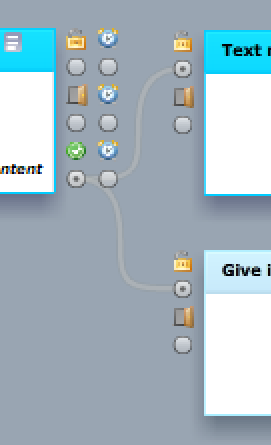
\includegraphics[width=0.18\textwidth]{StoryEditor_LinksBetweenNodes}
    \caption{Verbonden porten in de huidige story editor.}
    \label{fig:linksinstoryeditor}
\end{wrapfigure}

Door de bouwblokken aan elkaar te kunnen verbinden kunnen er een of meerdere verhaallijnen worden gemoduleerd. Verschillende bouwblokken worden met elkaar verbonden om volgorde en relatie tussen elkaar aan te geven. 

Formalismen leggen restricties op zowel het verbinden als het in elkaar voegen van bouwblokken. Dit kan duidelijk teruggezien worden in de huidige editors. Hierin wordt er gebruik gemaakt van porten om de nodes met elkaar te verbinden (\autoref{fig:linksinstoryeditor}). Zowel de story- als dialog editor lijkt gebruik te maken van semantische port groepen. Dit maakt het mogelijk om een betekenis te geven aan de porten. Beide hebben een 'in' en 'uit' groepen, waarbij de er geen verbinden kunnen worden gevormd tussen dezelfde groep; 'in' kan niet verbonden worden met een andere 'in'. Hiernaast werken sommige porten met tijd (zie de porten met klokjes in \autoref{fig:linksinstoryeditor}) en andere met logische expressies.

\begin{wrapfigure}{r}{0.32\textwidth}
    \centering    
    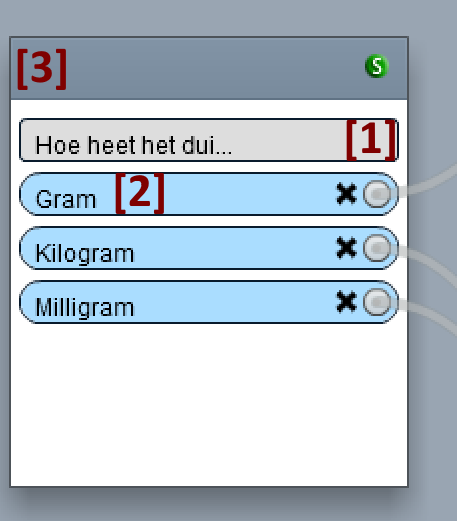
\includegraphics[width=0.28\textwidth]{DialogStateNodeEmbedding}
    \caption{Dialog editor: bouwblokken gevoegd in andere bouwblokken.}
    \label{fig:embeddedcomponents}
\end{wrapfigure}

In de dialog editor kunnen bouwblokken in elkaar gevoegd worden (zie \autoref{fig:embeddedcomponents}). Hier zitten wel bepaalde regels aan vast. Zo kunnen er alleen 'commands' (1) en 'options' (2) gevoegd worden in een 'state' (3). De 'command' en 'option' bouwblokken kunnen alleen bestaan als ze gevoegd zijn.

\subsubsection{Het valideren van verbindingen}
\noindent\textbf{Niveau}\\
Eerst moet er gekeken worden naar op welke niveau gevalideerd moet worden. Het niveau bepaald de granulariteit waarop de controle uitgevoerd wordt. Als er gekeken wordt op groepsniveau is het makkelijker om de rule set, of terwijl de verschillende restrictie regels, overzichtelijk en houdbaar in te delen. Hiertegenover staat dat er sprake is van een validatie op hoog niveau. Er wordt gekeken naar semantische groepen en niet naar de individuele porten. Dit maakt het moeilijk om eventuele uitzonderingen in de restricties toe te laten. Veel uitzonderingen kunnen echter weer zorgen voor onoverzichtelijkheid.

Het vastleggen van een rule set op groep niveau bevorderd de houdbaarheid, maar maakt het systeem ook minder flexibel. Het uitgangspunt van dit onderzoek is om alles zo flexibel mogelijk op te zetten, zolang dit geen hevige negatieven gevolgen heeft. Daarom zal het werken met semantische port groepen worden gestimuleerd, maar wanneer er een fijnere maten van controle vereist is moet het mogelijk zijn om op individueel niveau te valideren. Hierbij zal de validatie op individueel niveau de groepsvalidatie overschrijven.
\newline

\noindent\textbf{Validatie}\\
Om volledige controle te geven over het validatie proces zal het systeem gebruik maken van een validatie functie. Deze functie zal worden uitgevoerd wanneer de gebruiker een verbindingen gaat maken. De validatie functie kan uitgedrukt worden als:

\begin{quote} 
    \centering    
    \textit{
        validate: (x) =\textgreater{} boolean
    }
\end{quote}

Hierbij is 'x' het gene waar de verbinding tegen gevalideerd wordt. Omdat formalismen directe verbindingen met andere porten zouden kunnen toelaten, en het systeem hier geen restricties op moet leggen, kan 'x' zowel een port als een node zijn. Dit introduceert een nieuw probleem, omdat we niet weten wat voor type object meegegeven wordt als argument. Het maken van een validatie functie is lastig als het niet duidelijk is waartegen gevalideerd gaat worden. Echter is dit in een statically typed language, een programmeertaal waarin variabelen bestaan uit een type en een waarde, op te lossen door middel van method overloading. Hierbij wordt er voor elke mogelijke input een methode gemaakt (in dit geval twee methodes). Tijdens het compileren wordt er beslist welke methode waar gebruikt wordt. In een dynamically typed language bestaat het concept method overloading niet, omdat variabelen niet gebonden zijn aan een type. Dit betekent dat Typescript, wat uiteindelijk omgezet wordt in Javascript (een dynamically typed language), geen gebruik kan maken van method overloading. Echter biedt Javascript een uitweg met de 'instanceof' operator. Deze operator geeft een boolean, een logische waarde, terug die waar zal zijn als de constructor van het type terugkomt in de prototype chain. Een voorbeeld van een validatie functie geschreven in Typescript is terug te zien in 
\autoref{fig:validationfunction}. Deze functie beschrijft dat er alleen een verbinding mag worden gelegd met andere Nodes. Als er een validatie functie gedefinieerd is op individueel niveau zal deze de groepsvalidatie functie overschrijven.

\begin{figure}[htb]
    \centering
    \lstset{language=JavaScript}
    \begin{lstlisting}
    validateConnection(against: Port | Node): boolean => {
        if (against instanceof Port) {
            return false;
        }

        if (against instanceof Node) {
            return true;
        }
    }
    \end{lstlisting}
    \caption{Een voorbeeld van een validatie functie in Typescript.}
    \label{fig:validationfunction}
\end{figure}

\subsubsection{Het valideren van het in elkaar voegen}
Dezelfde methode en techniek kan gebruikt worden ter validatie van het in elkaar voegen van nodes.

\subsection{Hoe zou een algoritme eruitzien om vanuit een visuele structuur te compileren naar een formalisme?}
Nadat het verhaal geschreven is in de editor wordt deze geëxporteerd zodat het NGT hiervan gebruik kan maken. Dit exporteer proces zet de visuele structuur om naar JavaScript Object Notation (JSON), een gestandaardiseerd dataformaat. Het NGT kan dit formaat uitlezen en omzetten en interpreteren. Tijdens dit compilatie proces wordt editor specifieke informatie, zoals de positie en uiterlijk van nodes, niet mee geëxporteerd. Voor het NGT heeft deze informatie geen waarde en is dus overbodig.

\subsubsection{Het scheiden van bouwblokken en waarde}
In de huidige editors zit het formalisme vast gebakken in de visuele structuur. Bouwblokken hebben naast een uiterlijk ook een methode die een JavaScript object met data vrijgeeft. Dit object wordt vervolgens direct geserialiseerd; omgezet naar een formaat dat opgeslagen kan worden. De editor koppelt dus waarde en formalisme aan de bouwblokken zelf. Wat resulteert in niet herbruikbare bouwblokken; de bouwblokken zijn direct gekoppeld aan het formalisme.

Om het hergebruik van bouwblokken tussen meerdere formalismen mogelijk te maken moet de waarde van de bouwblokken gescheiden worden. Bouwblokken kunnen theoretisch terugkomen in meerdere formalismen waarin ze anders geïnterpreteerd moeten worden. Zo kunnen content typen terugkomen in zowel het formalisme van de story- als dialog editor. In de story editor zijn content typen terug te zien in de vorm van nodes, met verschillende in en uit porten (\autoref{fig:storyeditorcontenttype}). De dialog editor gebruikt content typen zonder porten (\autoref{fig:dialogeditorcontenttype}). Hier zijn de content typen ingevoegd in andere nodes.

\begin{figure}[htb]
    \centering    
    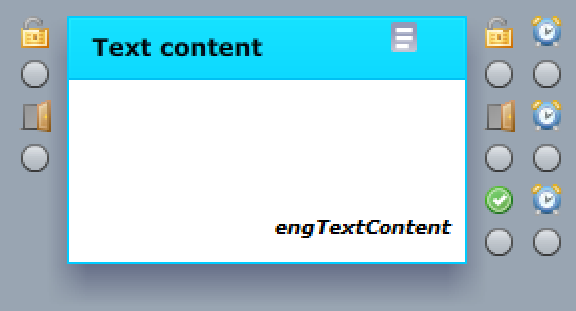
\includegraphics[width=0.45\textwidth]{StoryEditor_Node}
    \caption{Een content type in de story editor.}
    \label{fig:storyeditorcontenttype}
\end{figure}

\begin{figure}[htb]
    \centering    
    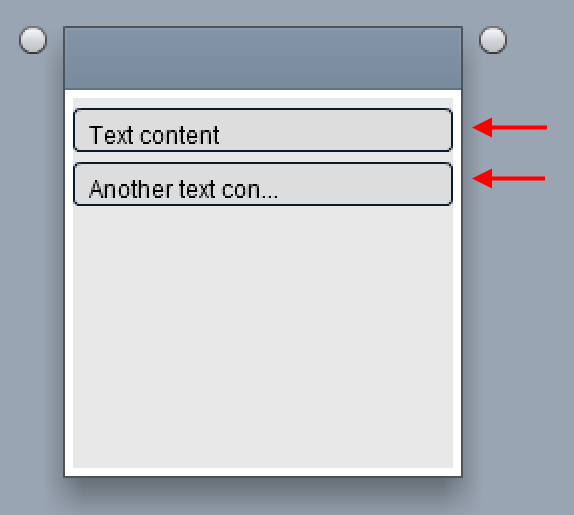
\includegraphics[width=0.45\textwidth]{DialogEditor_Node}
    \caption{Een content type in de dialog editor.}
    \label{fig:dialogeditorcontenttype}
\end{figure}

In \autoref{subsec:formulerenvanbouwblokken} wordt representatie van bouwblokken losgekoppeld van de werking door gebruik te maken van het ‘builder’ design pattern. De volgende stap is om de visuele structuur om te zetten naar een export-bestand volgens de richtlijnen van het desbetreffende formalisme. Hiervoor moet de serialisatie logica losgetrokken worden van de nodes zelf, zodat nodes geïnterpreteerd kunnen worden volgens het formalisme. Wanneer het verhaal wordt gecompileerd moet er volgens de richtlijnen van het formalisme waarde gekoppeld worden aan de bouwblokken. Hiernaast moet er worden gekeken hoe de graaf doorlopen gaat worden.

\subsection{Compilatie stap}
De interpretatie van nodes moet losgekoppeld worden van de visuele structuur. Dit betekent dat de nodes zelf geen methode moeten bevatten die de data van een node vrijgeeft. Nodes moeten geïnterpreteerd worden volgens zowel interface als formalisme. 

Door gebruikt te maken van het visitor design pattern wordt er een context aangeboden waarin het exporteer-bestand opgebouwd kan worden. De 'gang of four' koppelt de volgende intent aan dit design pattern\cite{DesignPatterns}:

\begin{quote} 
    \centering    
    \textit{
        "Represent an operation to be performed on the elements of an object structure. Visitor lets you define a new operation without chaning the classes of the elements on which it operates."     
    }
\end{quote}

Deze intentie kan gekoppeld worden aan het eerder beschreven probleem. De operatie die uitgevoerd wordt op de elementen van een object structuur, betreft het omzetten van de visuele structuur naar een export-bestand. Hierbij worden operaties gedefinieerd in de visitor in plaats van in de nodes zelf waarmee interpretatie van de nodes losgekoppeld wordt.

\subsubsection{Visitor pattern}
Het visitor pattern definieert de volgende deelnemers:

\begin{itemize}
    \item \textbf{Visitor} (ExportGeneratingVisitor)
    \begin{itemize}
        \item Definieert voor iedere concrete element klasse in de datastructuur een 'Visit' methode. Echter werken we met JavaScript, een programmeertaal die loosly typed is; data typen worden niet expliciet gedefinieerd. Hierdoor kan er geen gebruik worden gemaakt van method overloading. Dit heeft als gevolg dat de Visitor interface maar één 'Visit' methode zal definieren. In de concrete visitor zullen de type specifieke operaties worden gedefinieerd, zoals in \autoref{fig:validationfunction}.
    \end{itemize}

    \item \textbf{Concrete Visitor} (StoryExportGeneratingVisitor)
    \begin{itemize}
        \item Implementeerd de 'Visitor' interface en biedt content voor het algoritme. Hiernaast kan de concrete visitor staat verzamelen, in dit geval bouwt deze het export-bestand op.
    \end{itemize}

    \item \textbf{Element} (Node)
    \begin{itemize}
        \item Definieert een 'Accept' methode met de Visitor als parameter.
    \end{itemize}

    \item \textbf{ConcreteElement} (Bouwblokken in formalisme, zoals 'ContentNode')
    \begin{itemize}
        \item Implementeert de 'Element' interface, met de 'Accept' methode die een visitor as parameter neemt.
    \end{itemize}

    \item \textbf{ObjectStructure} (Graph)
    \begin{itemize}
        \item Biedt een interface om te itereren over haar elementen.
    \end{itemize}
\end{itemize}

Het totaal plaatje is terug te zien in \autoref{fig:appliedvisitorpaternuml}. Voor ieder formalisme wordt een concrete visitor aangemaakt, zodat ieder formalisme de elementen kan interpreteren volgens haar eigen richtlijnen.

\begin{figure}[htb]
    \centering    
    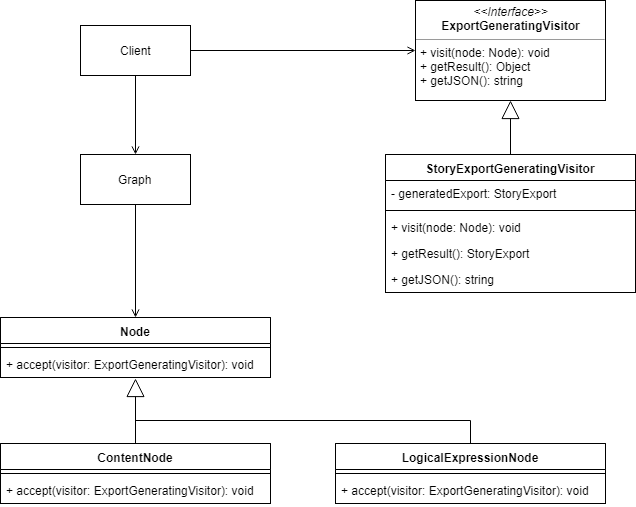
\includegraphics[width=0.9\textwidth]{ExportGeneratingVisitor}
    \caption{Het visitor pattern toegepast voor het formalisme van de story editor.}
    \label{fig:appliedvisitorpaternuml}
\end{figure}

\subsubsection{Consequenties}
Het gebruik van het visitor pattern om van visuele structuur naar export-bestand te compileren heeft de volgende consequenties:
\begin{enumerate}
    \item Bouwblokken kunnen worden toegevoegd aan een formalisme, zonder zelf van het formalisme af te weten. Hiermee wordt vervuiling van de nodes voorkomen. 
    \item Bouwblokken kunnen worden hergebruikt in andere formalisme. De concrete visitor voor het desbetreffende formalisme moet dan wel een methode definiëren die de bouwblokken kan bezoeken.
    \item Elke bouwblok moet een ‘Accept’ methode implementeren.
    \item Concrete visitors kunnen staat bijhouden. Dit wordt gebruikt om het export-bestand op te bouwen.
\end{enumerate}

In een strongly typed programmeertaal zou het toevoegen van concrete elementen lastiger zijn. Hiervoor moet de interface van de visitor aangepast worden om het nieuwe element te ondersteunen. Dit zou ook betekenen dat iedere concrete visitor (en dus elk formalisme) een visit methode zou moeten implementeren voor ieder bouwblok. Als bouwblokken niet worden gebruikt in een formalisme zou dit lege methode opleveren. Echter wordt deze consequentie ontweken doordat er gewerkt wordt in JavaScript, een loosly typed programmeertaal.

Het prototype implementeert het visitor pattern en valideert zo het gebruik van het visitor pattern voor de compilatie stap.

\section{Conclusie}
Met dit hoofdstuk wordt de volgende deelvraag beantwoord: “Hoe kan de architectuur achter de editor zo worden opgezet dat er in latere stadia nieuwe narratieve formalismen makkelijk doorgevoerd kunnen worden?”.

Een formalisme bestaat (1) uit syntactische vormen legt (2) restricties op het verbinden en het in elkaar voegen van deze vormen. Met behulp van het builder design pattern kunnen bouwblokken worden gescheiden van representatie. Dit laat het hergebruik van bouwblokken met verschillende representaties toe. Hiernaast biedt de builder een expliciete interface voor het construeren van nodes en kapselt deze het constructieproces af. Ieder formalisme beschikt over een eigen director die een set aan beschikbare bouwblokken formuleert voor het desbetreffende formalisme.

Restricties tussen het verbinden van deze syntactische vormen kunnen worden opgelegd door gebruik te maken van een validatie functie. Wanneer de bouwblokken gebruik maken van porten worden er semantische port groepen gedefinieerd om restricties op groepsniveau toe te laten. Restricties op individueel niveau overschrijven de restricties gedefinieerd op groepsniveau. 

De visuele weergave van bouwblokken kan worden losgekoppeld van één ingebakken formalisme door gebruik te maken van het visitor design pattern. Hierdoor worden bouwblokken en waarde losgekoppeld. Tijdens het compileren van de visuele structuur naar een export-bestand zal er waarde worden gehangen aan de bouwblokken volgens de richtlijnen van het desbetreffende formalisme. Dit laat het hergebruiken van bouwblokken tussen verschillende formalismen toe.

Door formalisme specifieke logica los te koppelen van de visuele weergave van bouwblokken kunnen er in latere stadia nieuwe bouwblokken geformuleerd worden en nieuwe formalisme doorgevoerd worden.


\chapter{Overkoepelende Projectstructuur}
\label{ch:overkoepelendeprojectstructuur}
In dit hoofdstuk wordt er een voorstel gedaan om de editors deel uit te laten maken van een overkoepelende projectstructuur; de editors zullen het gehele project openen in plaats van een enkel bestand. Door de editors beschikbare bestanden te laten beheren kunnen er sterkere referenties worden gemaakt tussen de game content en de editor. Een overkoepelende projectstructuur laat functionaliteiten toe die eerst niet mogelijk waren, zoals het previewen van assets in de editor en het gebruiken van gedeelde variabelen in zowel verhaal als dialoog. Om het beheren van bestanden mogelijk te maken wordt er een voorstel gedaan om de huidige folderstructuur van het NGT te veranderen. Verder worden er twee semantische lagen geïntroduceerd die de foutgevoeligheid van de nieuwe editor verminderd.

\section{Projectstructuur narrative game}
Narrative game projecten wordt ontwikkeld in het NGT. Dit template dwingt een folderstructuur af die vrijwel ieder project aanhoudt. In deze folderstructuur bevindt zich de code en content voor de game. De bestanden die samen de game content omschrijven worden ook wel ‘assets’ genoemd. Voorbeelden van assets zijn: afbeeldingen, video’s, geluidsbestanden en configuratie bestanden. Kortom, alle media en data die het spel (in)direct aan de speler toont. Vaak worden deze assets al geordend in mapjes wat al wijst op een behoefte aan een projectstructuur.

\section{Koppeling tussen assets en de editors}
De huidige editors openen een save-bestand. Voor de story editor is dit een ‘.sty’ bestand, de dialog editor opent een ‘.dlg’ bestand. Beide schrijven het export-bestand weg naar een los JSON-bestand. Assets worden handmatig gespecificeerd in een aparte JSON, ook wel assets.json genoemd (zie bijlage \autoref{app:assetsjson}). Beide editor refereren naar assets door middel van een sleutel die correspondeert met een sleutel in de assets.json. 

Dit betekent dat de editors niks af weten van de assets in het project. Er is een folder vol assets die allemaal worden ingeladen. Deze selectie ingeladen assets kunnen worden verwerkt in verhaal of dialoog. Er zijn use cases voor een overkoepelende projectstructuur opgesteld en gevalideerd in de wekelijkse meetings met de bedrijfsbegeleider en opdrachtgever (bijlage \autoref{app:usecasesprojectstructuur}). Hieruit blijkt dat het gebruikt van onbeheerde assets invloed heeft op de foutgevoeligheid, efficiëntie en functionaliteit van de editors. 

\subsection{Foutgevoeligheid}
Content typen met referenties naar assets, zoals ‘image content’ welke refereert naar een image asset, zijn erg gevoelig voor menselijke fouten. Deze content typen tonen voor iedere referentie een invoerveld die één lijn aan tekst bevat. Hierin kunnen gebruikers de sleutel invoeren die bij de juiste asset hoort. De invoer kan niet worden gecontroleerd door de editor wat twee problemen introduceert. Typefouten of referenties naar niet bestaande assets worden toegelaten. Hiernaast wordt het invoeren van verkeerde typen assets toegestaan. Zo zou ‘image content’ een referentie kunnen bevatten naar een mp3-bestand. De editor kunnen geen semantiek toewijzen aan assets.

Beide scenario’s worden niet afgevangen in de editors en kunnen resulteren in ongewenst gedrag en mogelijke crashen in de game. Dit hakt in op de efficiëntie van de editors.

\subsection{Inefficiëntie}
De foutgevoeligheid haakt in op de efficiëntie van de editors. Door een foutgevoelige editor moeten er meer testen en eventuele correcties uitgevoerd worden om een stabiele game aan te kunnen leveren.
Hiernaast is er geen mogelijkheid om ongebruikte assets te filteren, ongebruikte assets blijven altijd in de game zitten. Sommige hiervan zullen zelfs worden ingeladen als ze in het JSON-bestand staan. Dit zorgt voor een langere en onnodige laadtijd van de game.

\subsection{Disfunctionaliteit}
Zoals beschreven in \autoref{ch:technologystack}, speelt klant co-creatie een rol in de toekomst van de editor. Hiervoor is het belangrijk dat de editors beschikken over een sterke visualisatie van het verhaal\cite{Schipper2015}. Dit is lonend voor zowel klant als game design. Deze visualisatie moet naast overzicht ook inzicht bieden in de game content, zo zal ‘image content’ een preview moeten laten zien van de gerefereerde afbeelding. Om dit mogelijk te maken moet er enigszins sprake zijn van een overkoepelende projectstructuur waarbij assets beheerd worden door de editor. 


\section{Behoefte aan een overkoepelende projectstructuur}
Door mee te werken aan een narrative game project kwamen er enkele behoeftes naar boven. In de wekelijkse meetings zijn deze gevalideerd en aangevuld. Hieruit zijn use cases opgesteld (zie bijlage \autoref{app:usecasesprojectstructuur}) die gebruikt worden om de behoefte aan een overkoepelende projectstructuur naar voren te brengen. 

\begin{wrapfigure}{r}{0.35\textwidth}
    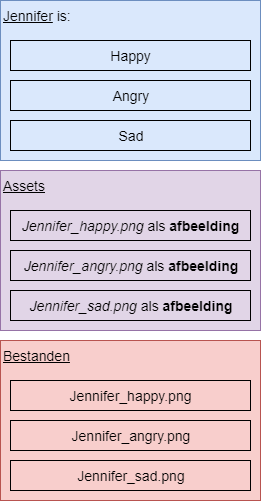
\includegraphics[width=0.33\textwidth]{SemanticLayersWithoutArrows}
    \caption{De verschillende asset betekenis lagen.}
    \label{fig:semanticgamecontentlayersdetailed}
    \centering
\end{wrapfigure}

In een digitale interactive narratief wordt er gebruik gemaakt van variabelen om conditionaliteit mogelijk te maken. Het beschikken over gedeelde variabelen tussen verhaal en dialoog is nodig om het verhaal te kunnen sturen volgens gemaakte keuzes in de dialoog en wederzijds. Deze gedeelde variabelen worden gezien als een overkoepelend construct en wekt de vraag naar een overkoepelende projectstructuur op waarbij variabelen, verhalen en dialogen samen komen en met elkaar verbonden worden.

Het kan vervelend worden ondervonden om gebruik te moeten maken van twee verschillende applicaties die op veel fronten overlappen. Voor het verhaal maakt men gebruik van de story editor, voor dialogen de dialog editor. Een overkoepelende projectstructuur maakt het mogelijk om verhaal en dialoog bestanden met elkaar te verbinden. Naast story telling tools kunnen ook integrated development environments (IDE's) gebruik maken van een overkoepelende projectstructuur. In veel IDE's is dit terug te zien aan de ingebouwde verkenner, waarin de gebruiker bestanden kan selecteren en openen.

Referenties naar assets worden gemaakt door het invoeren van een tekstuele sleutel. Daarbij moet de asset worden gespecificeerd in het assets JSON-bestand. Dit is relatief makkelijk te vergeten en daarnaast worden er veel typfouten gemaakt. Daarnaast kan de gebruiker zonder waarschuwing een verkeerd type asset invoeren, zoals een afbeelding in een geluid veld. De editor moet een lijst aanreiken met beschikbare assets van het juiste type, om zo de foutgevoeligheid te verminderen.

Naast het onderscheid maken tussen typen assets is het wenselijk om entiteiten te kunnen koppelen aan assets. Hierbij bestaat bijvoorbeeld een karakter uit meerdere emoties die uitgedrukt worden in afbeeldingen (\autoref{fig:semanticgamecontentlayersdetailed}).

\section{Stappen richting een overkoepelende projectstructuur}
Om aan deze behoeftes te voldoen moeten er stappen worden gezet richting een overkoepelende projectstructuur. De editor moet hiervoor bij bestanden kunnen die zich bevinden in de projectfolder. Wat betekend dat de editor de gehele projectfolder zal moeten openen in plaats van alleen het save-bestand. De folderstructuur van het project moet dit wel ondersteunen; bruikbare assets moet gescheiden worden van niet bruikbare bestanden zoals code. Daarnaast moet er een folder komen waarin alle overkoepelende constructen, zoals variabelen en content typen schema's, worden opgeslagen.

De editor moet bestanden in de projectfolder inventariseren en onderscheid maken tussen zowel bruikbare bestanden als typen bestanden. Daarnaast moet er een manier komen om assets te koppelen aan entiteiten. Wanneer bestanden worden verplaatst, aangepast of verwijderd worden moet de inventarisatie en referenties naar deze assets worden geüpdatet als nodig.

Het afdwingen van typen assets in de inspector vereist een uitbreiding van JSON-schema. In het schema moet het type asset kunnen worden gedefinieerd.

Tenslotte zal moeten worden gekeken naar het exporteer proces van game content. Hierin zal er een pakketje moeten worden gemaakt waarin zich alle game content bevindt.

\section{Een ondersteunende folderstructuur}
In een overkoepelende projectstructuur wordt de gehele project folder geopend in plaats van een specifiek bestand. Door de project folder te openen kunnen assets binnen het project geïnventariseerd en beheerd worden. Hiernaast kan de inventarisatie aangepast worden als er assets verwijderd of toegevoegd worden. In \autoref{sec:assetmanagement} wordt er dieper in gegaan op het beheren van assets.

Bij het openen van de gehele project folder is het alleen wenselijk om assets te beheren die verwerkt kunnen worden in het verhaal. Bestanden die broncode of configuraties voor command line tools representeren kunnen niet worden verwerkt in het verhaal. De editor hoeft niks van deze bestanden af te weten. In de huidige folderstructuur van het ‘narrative game template’ (NGT), het raamwerk waarin narrative games gerealiseerd worden, bevinden zich bruikbare en niet bruikbare bestanden in deze zelfde folder. Om een gestructureerde overkoepelende projectstructuur toe te laten zullen er aanpassingen moeten worden gedaan op de folderstructuur. Deze aanpassing zijn alleen bedoelt om een overkoepelende projectstructuur te ondersteunen.

\section{Folderstructuur van het narrative game template}
In \autoref{fig:ngtfolderstructure} wordt de folderstructuur van het NGT weergeven. De ‘src’ (source) directory bevat de broncode en game content van de game. Hierin bevinden zich een ‘assets’ en een ‘ranj’ directory. De ‘ranj’ directory bevat de broncode van het spel en zal dus geen deel uit moeten maken van de overkoepelende projectstructuur. In de ‘assets’ directory zitten, zoals de naam luidt, alle asset die worden verwerkt in de game. Hiernaast bevinden zich project specifieke configuraties en flash files\footnote{Visual designers gebruikt Adobe Animate CC om schermen te ontwikkelen voor narrative games.} ook in deze directory. Deze project specifieke configuraties en flash files zijn niet verwerkbaar in het verhaal en moeten dus uit de assets directory. Project specifieke configuraties zouden eventueel wel gebruikt kunnen worden door de editors. Een voorbeeld hiervan is het content typen dataschema beschreven in \autoref{ch:diversiteitingamecontent}. 

Dit creëert de behoefte voor een nieuwe directory genaamd ‘ProjectSettings’. Hierin zullen zich project specifieke configuratie bestanden bevinden. Waarbij sommige bestanden, zoals het content typen dataschema, uitgelezen zal worden door de editors. Dit maakt het definiëren van een selectie aan project specifieke content typen op projectniveau mogelijk.

\begin{figure}[htb]
    \dirtree{%
    .1 /.
    .2 autoplay.
    .2 build-tools.
    .2 dev-tools.
    .2 src.
    .3 assets.
    .3 css.
    .3 lib.
    .3 ranj.
    .3 swf.
    .3 test.
    .2 translations.
    }
    \caption{Folderstructuur van het NGT.}
    \label{fig:ngtfolderstructure}
\end{figure}

\section{Het beheren van assets}
\label{sec:assetmanagement}
Om de assets te beheren zal de editor een lijst moeten bijhouden met daarin informatie over beschikbare assets in de ‘assets’ directory. Elementen in deze lijst worden gerepresenteerd als:
\begin{quote} 
    \centering    
    \textit{
        \{ id : string, path : string, type : string \} 
    }
\end{quote}
\noindent Waar;
\begin{description}
    \item[id] bestaat uit een unieke string die eenmaal gegeneerd zal worden wanneer de asset geïnventariseerd wordt. Deze wordt gebruikt om naar assets te refereren. Dit speelt een rol in het exporteer proces beschreven in \autoref{sec:exportproces}.
    \item[path] een relatief pad naar de asset vanaf de root van het project is. Zo kan zowel de editor als het NGT de locatie van de asset achterhalen. Wanneer er naar deze asset gerefereerd wordt kan de bestandsnaam uit dit pad getoond worden om inzicht te geven in de gerefereerde asset.
    \item[type] semantiek toekent aan de asset (e.g. ‘image’, ‘sound’).
\end{description}

Door gebruik te maken van een ‘id’ blijven referenties intact wanneer het pad naar het bestand veranderd. Als de asset verwijderd wordt zullen referenties naar deze asset breken. De editor kan vervolgens aangeven welke referenties gebroken zijn en eventueel vragen met welke asset deze vervangen moeten worden. Een nadeel aan het gebruik van een onleesbare sleutel is dat de assets niet statisch opgehaald kunnen worden in het NGT. Het NGT kan sleutel uitlezen uit het exporteer bestand en deze omzetten naar de afbeelding (zie \autoref{sec:exportproces}), maar een programmeur kan geen afbeelding inladen door een statische sleutel mee te geven. Als dit wel wenselijk is zou er eventueel een ‘tag’ property kunnen worden toevoegt aan de elementen in de lijst. Deze zou dan wel handmatig moet worden ingesteld in de editor, wat een user interface zal vereisen.

Deze lijst zal tijdens de eerste keer opstarten van de editor opgebouwd en weggeschreven worden naar een JSON-bestand in de ‘ProjectSettings’ folder. Wanneer de lijst aanwezig is in de ‘ProjectSetting’ zal deze worden ingeladen tijdens het opstarten van de editor.

Om de lijst bij te houden terwijl de editor open is zal de ‘assets’ folder worden ‘gewatched’. Dit houdt in dat de editor een event afvuurt wanneer er een bestand aangemaakt, bewerkt, verplaatst of verwijderd wordt. NodeJS beschikt over een module genaamd ‘filesystem’ die deze functionaliteit aanbied. Daarentegen blijkt deze functionaliteit van NodeJS vrij inconsistent is, dit meldt NodeJS ook in de documentatie\cite{NodeDocFS}. Met twee events, zijnde ‘change’ en ‘rename’, is het lastig om te achterhalen wat precies het event afvuurde. 

Er kan gebruik gemaakt worden van een library, zoals Chokidar\footnote{https://github.com/paulmillr/chokidar}, die meer consistentie biedt. Deze library biedt een interface met expliciete events zoals ‘add, ‘change’ en ‘unlink’. Hiernaast zijn er ook events voor directory beschikbaar zoals ‘addDir’ en ‘unlickDir’. Chokidar wordt gebruikt in veel projecten\footnote{https://www.npmjs.com/browse/depended/chokidar}, waaronder Microsoft’s visual studio code\footnote{https://github.com/microsoft/vscode}. 

\subsection{Optimalisatie}
\label{subsec:optimalisationformat}
Het refereren naar assets is een veel voorkomende actie in de editors. Wanneer de gebruiker in ‘image content’ naar een afbeelding wilt refereren zal de lijst gefilterd moeten worden op assets met het type ‘image’ (\autoref{lst:filterassetimage}). Het iedere keer moeten filteren van een potentiele grote lijst aan assets kan mogelijk, afhankelijk van de grootte van de lijst, zorgen voor een slechte gebruikerservaring. De tijdcomplexiteit van het algoritme in \autoref{lst:filterassetimage} kan worden uitgedrukt als \textit{O(n)}, waarin ‘n’ het aantal elementen in de array zijn. 

\begin{figure}[htb]
    \centering
    \lstset{language=JavaScript}
    \begin{lstlisting}
    availableAssets.filter(asset => asset.type === 'image');
    \end{lstlisting}
    \caption{Het filteren van assets met het type 'image'.}
    \label{lst:filterassetimage}
\end{figure}

Om het vinden van assets met een bepaald type efficiënter te maken kan de editor een JavaScript object bijhouden die dient als een ‘lookup table’. In dit object dienen de properties als keys die ieder een array van assets bevatten met dat type (zie \autoref{lst:optimizedmanageformat}). De tijdcomplexiteit van een property lookup zoals in \autoref{lst:propertylookup} kan worden uitgedrukt als \textit{O(1)}.

\begin{figure}[htb]
    \centering
    \lstset{language=JavaScript}
    \begin{lstlisting}
    {
        images: [
            ..
        ],
        videos: [
            ..
        ]
    }
    \end{lstlisting}
    \caption{Geoptimaliseerd formaat voor het beheren van assets.}
    \label{lst:optimizedmanageformat}
\end{figure}

\begin{figure}[htb]
    \centering
    \lstset{language=JavaScript}
    \begin{lstlisting}
    const availableImages = availableAssets.images;
    \end{lstlisting}
    \caption{Het verkrijgen van alle beschikbare images door middel van een property lookup}
    \label{lst:propertylookup}
\end{figure}

\section{Semantiek binden aan assets}

\begin{wrapfigure}{r}{0.35\textwidth}
    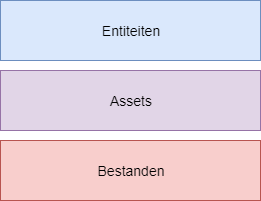
\includegraphics[width=0.33\textwidth]{SemanticLayersInGameContent}
    \caption{Semantische lagen in game content.}
    \label{fig:semanticgamecontentlayers}
    \centering
\end{wrapfigure}

Om de editors minder foutgevoelig te maken wordt er semantiek in de vorm van een type toegewezen aan de assets. Zo moeten de nieuwe editors alleen het gebruikt van afbeeldingen in ‘image content’ toelaten. Door een type toe te wijzen aan assets kunnen types worden afgedwongen in de editor. 

In deze paragraaf is er sprake van twee semantische lagen boven die gebonden worden aan bestanden die beschikbaar zijn voor de editor: de asset- en entiteiten laag. De asset laag classificeert bestanden op bestandstypen zoals afbeelding of video. De entiteiten laag categoriseert en koppelt deze assets aan hogere constructen zoals karakters en locaties. 

Voor de eerste semantische laag, het hangen van types aan bestanden, moeten de volgende stappen worden ondernomen:

\begin{enumerate}
    \item De nieuwe editor moet een type kunnen hangen aan bestanden wanneer deze ingeladen worden.
    \item Het content typen dataschema moet typen kunnen \item De inspector moet het afgedwongen typen in het dataschema respecteren en eventuele andere typen weigeren.
\end{enumerate}

Boven op de assets laag wordt de entiteiten laag gebouwd.

\begin{enumerate}[resume]
    \item Assets moeten gecategoriseerd en gekoppeld kunnen worden aan hogere constructen.
\end{enumerate}

\subsection{Bestanden koppelen aan een type}
Er kan een type aan een assets gekoppeld worden door de extensie van het bestand te respecteren. Zo is een ‘.png’ of ‘.jpeg’ een afbeeldingen en een ‘mp4’ een video. Deze semantische laag wordt vanaf nu de ‘asset laag’ genoemd. De nieuwe editor zal in code over een map moeten beschikken waarin een bestand extensie gekoppeld staat aan een type. Alleen extensies die ondersteund worden door het NGT zullen moeten worden opgenomen in deze map. Deze map wordt gedefinieerd in broncode, omdat deze wordt geacht om statisch te zijn. Als de map aangepast moet worden zal de programmeur dit moeten doen, omdat hier verdere consequenties aanhangen. Het toevoegen van een nieuwe mapping zal invloed hebben op het NGT, deze moet de nieuwe extensie ondersteunen. Hiernaast zal het omzetten van een mapping moeten resulteren in een migratie van de interne lijst aan beheerde assets.

\subsection{Het uitbreiden van JSON-schema functionaliteit}
Het content typen dataschema moet uitgebreid worden om informatie over het type asset te verstrekken. Refereren naar assets gebeurd door middel van een sleutel; de ‘id’ waarde van de elementen in de lijst. Een sleutel is een string wat betekend dat het JSON-schema voor een referentie property nog steeds ‘string’ waarde voor het ‘type’ keyword bevat. Er moet een keyword toegevoegd worden om metadata te verstrekken over het type asset.

JSON-schema verstrekt zelf al een ‘format’ keyword die semantische validatie toelaat. Een voorbeeld van een formaat is: ‘email’\cite{Droettboom2016}. De waardes van format mogen uitgebreid worden naar benodigde formaten. Maar omdat een ‘id’ niet in een onderscheidbaar formaat staat is het beter om een nieuw keyword toe te voegen waarin het type asset omschreven kan worden. Hiervoor wordt er een nieuw keyword geïntroduceerd: ‘assetType’. Voorbeelden van waardes van dit keyword zijn: ‘image’, ‘video’, ‘sound’, ect ...

\subsection{Het afdwingen van typen in de inspector}
Om JSON-schema’s te reflecteren in de inspector wordt gebruik gemaakt van de ‘react-jsonschema-form’ library, zoals vermeld in \autoref{ch:diversiteitingamecontent}. Het toevoegen van een nieuw keyword in het JSON-schema woordenboek betekend dat er nieuwe componenten gemaakt moeten worden die dit keyword ondersteunen. Deze component moet getoond worden wanneer het ‘assetType’ keyword aanwezig is in het schema.

Het ondersteunen van dit nieuwe keyword heeft een grote impact op de library. Om het ‘assetType’ keyword te ondersteunen moet het standaard gedrag van de library worden aangepast; het standaard veld voor een string type moet worden overschreven. De component die het string veld overschrijft zal de juist component teruggeven voor het schema.

\pagebreak

\subsection{Het koppeling van assets aan entiteiten}
Vaak worden afbeeldingen van karakters en locaties geordend in een folderstructuur. Dit duidt op een behoefte aan het categoriseren van assets. Met een tweede semantische laag worden asset van hetzelfde typen handmatig gebonden aan hogere entiteiten zoals karakters en locaties. Hiermee kan worden voorkomen dat er per ongeluk een verkeerde afbeelding bij een bepaald karater wordt gebruikt.

Omdat het refereren naar assets gaat via een menselijk onleesbare sleutel zal het handmatig binden van assets aan entiteiten moeten gebeuren door middel van een user interface in de editors. Deze user interface zal de gebruiker meer informatie geeft over de asset waarmee de gebruiker deze asset kan identificeren. Wanneer deze gekoppeld wordt aan een entiteit zal de editor de bijbehorende sleutel zoeken.

Deze semantische laag leeft niet in het content typen schema zoals de eerste semantische laag, maar op project niveau. Een geserialiseerd (zoals te zien in \autoref{lst:serializedentitylayer}) formaat zal dan ook worden opgeslagen in de ‘ProjectSettings’ folder. Het geserialiseerde formaat in \autoref{lst:serializedentitylayer} is geoptimaliseerd zoals beschreven in \autoref{subsec:optimalisationformat}.

\begin{figure}[htb]
    \centering
    \lstset{language=JavaScript}
    \begin{lstlisting}
    {
        "images": [
            {
                "jennifer": [
                    "idAsset1",
                    "idAsset2"
                ]
            }
        ],
        "videos": [
            ..
        ]
    }          
    \end{lstlisting}
    \caption{Geserialiseerde representatie van de entiteiten laag.}
    \label{lst:serializedentitylayer}
\end{figure}

\begin{wrapfigure}{r}{0.42\textwidth}
    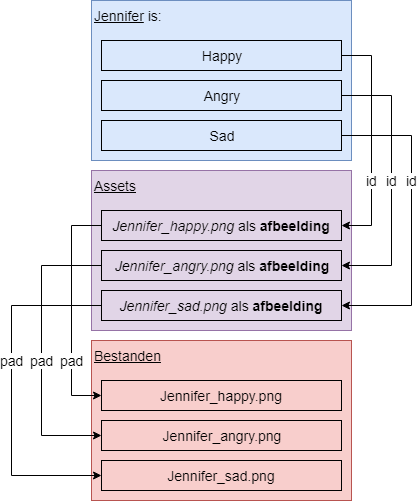
\includegraphics[width=0.4\textwidth]{EntityLayerExample}
    \caption{Relaties tussen de verschillende semantische lagen.}
    \label{fig:semanticlayerrelationships}
    \centering
\end{wrapfigure}

Vervolgens zullen content typen met een referentie naar een asset een extra veld moeten tonen in de inspector. Dit extra veld is een drop down menu waarin een keuze gemaakt kan worden uit de eerder gecreëerde entiteiten. Vervolgens kunnen de assets gefilterd worden op de geselecteerde entiteit. Dit extra veld wordt niet gedefinieerd in het content typen schema en niet geëxporteerd. Het wordt wel opgeslagen in de save file die de editor produceert.

De relaties tussen de semantische lagen zijn terug te zien in \autoref{fig:semanticlayerrelationships}.

\clearpage
\section{Het exporteren van game content}
\label{sec:exportproces}
Voorheen exporteerde de huidige editors slechts twee bestanden die het verhaal en gelokaliseerde inhoud omschreven. Een overkoepelende projectstructuur maakt het mogelijk om gebruikte assets, het verhaal en configuratie bestanden samen te bundelen in een archief format zoals tar\footnote{https://www.freebsd.org/cgi/man.cgi?query=tar\&apropos=0\&sektion=5\&manpath=FreeBSD+7.0-RELEASE\&arch=default\&format=html} of asar\footnote{https://github.com/electron/asar}. Er is niet gekeken naar een “best passende formaat” in deze context. Naast dat dit het laden van ongebruikte assets voorkomt verkleint dit het aantal HTTP requests, die gemaakt moeten worden om alle files binnen te halen. Een HTTP request bevat extra informatie welke iedere keer mee gestuurd zal worden\cite{Fielding1999}. Dit maakt het ophalen van één groter bestand sneller dan vele kleinere bestanden wat zorgt voor een snellere laadtijd van het spel.

Het NGT maakt gebruik van een library genaamd: ‘preloadJS’\footnote{https://www.createjs.com/preloadjs}. Met deze library worden bestanden ingeladen. De library biedt de mogelijkheid om een zogenaamde ‘manifest’ op te stellen. Dit is een JSON-bestand waarin paden naar bestanden worden gekoppeld aan een sleutel. De nieuwe editor kan een manifest specificeren, omdat deze beschikt over de sleutels en paden van gebruikte assets. Paden naar assets worden gestript van (sub)directories die zich bevinden in het pad, zodat alleen de bestandsnaam met extensie overblijft. Vervolgens wordt het basis pad gespecificeerd door de export locatie te pakken en de locatie van het NGT project hiervan af te trekken. Dit resulteert in een relatief pad dat het NGT leidt naar de locatie van de assets. Een voorbeeld van een manifest is terug te zien in \autoref{lst:manifestexamplepreloadjs}. Omdat dit proces zo alleen zou werken voor de ‘preloadJS’ library is het aan te raden om voor het genereren van een manifest gebruik te maken van het ‘strategy design pattern’, om zo ondersteuning voor eventuele andere libraries te bieden.

\begin{figure}[htb]
    \centering
    \lstset{language=JavaScript}
    \begin{lstlisting}
    {
        "path": "assets/",
        "manifest": [{
                "id": "8e3c642d-ab1e-4c81-a379-0b236bf692f8",
                "src": "jennifer_happy.png"
            },
            {
                "id": "23951903-0f4e-43d2-9602-5fd6e70b0d32",
                "src": "jennifer_angry.png"
            }
        ]
    }               
    \end{lstlisting}
    \caption{Voorbeeld van een manifest in preloadJS.}
    \label{lst:manifestexamplepreloadjs}
\end{figure}

\pagebreak
\section{Conclusie}
Met deze conclusie wordt deelvraag “Hoe kan game content in een overkoepelende projectstructuur verbonden en geordend worden?“ beantwoord.

Het gebruiken van een overkoepelende projectstructuur in de nieuwe editors bevorderd efficiëntie, functionaliteit en verminderd foutgevoeligheid. De folderstructuur van het NGT zal aangepast moeten worden om deze overkoepelende projectstructuur te ondersteunen.

Om game content te ordenen en met elkaar te verbinden in een overkoepelende projectstructuur zal de editor assets, bestanden die samen de game content opbouwen, moeten beheren. Dit wil zeggen dat de nieuwe editor een lijst met beschikbare assets zal bijhouden. Elementen in deze lijst bestaan uit een gegenereerde “menselijk onleesbare” unieke sleutel, een pad naar het bestand en het type bestand (e.g. afbeelding) die semantiek toe kent aan de asset. De sleutel maakt het verbinden van assets mogelijk. Deze sleutel wordt gebruikt om te refereren naar de bijbehorende asset en zorgt dat referenties niet breken wanneer de asset verplaatst wordt. Een nadeel aan een menselijk onleesbare sleutel is dat alleen de editor kan refereren naar deze assets. De programmeur kan moeilijk refereren naar deze assets vanuit statische context. Bij iedere verandering in de lijst zal deze worden geserialiseerd en weggeschreven naar een bestand in de overkoepelde project folder, zodat deze uitgelezen kan worden wanneer de editor het project opent. Als dit bestand wordt verwijderd zullen alle referenties binnen de editors breken.

Semantiek wordt toegekend aan de assets door (1) automatisch een type te binden aan assets door middel van de bestandsextensie en (2) een handmatige stap waarbij assets aan entiteiten gebonden worden. Een voorbeeld van een entiteit is een karakter welke bestaat uit verschillende afbeeldingen die emoties representeren.

Wanneer de nieuwe editor het verhaal exporteert zullen alle gebruikte assets, configuratie bestanden en het verhaal samen gebundeld worden in een archief format zoals tar. Dit verminderd het aantal HTTP requests dat het NGT hoeft te maken om assets in te laden. Het NGT gebruikt de library ‘preloadJS’ om bestanden in te laden. Deze heeft een manifest nodig die opgesteld moet worden tijdens de exporteer stap.

\section{Vervolgonderzoek}
\subsection{User interfaces voor beheren van de entiteiten laag}
Het binden van assets aan entiteiten is een handmatig proces waarbij de gebruiker via een user interface assets moet kunnen koppelen aan (zelf aangemaakte) entiteiten. Hiervoor dient de gebruiker over een user interface te beschikken waarbij de gebruiker assets kan koppelen aan entiteiten, omdat het lastig is om te werken met menselijk onleesbare asset sleutels. Er is geen onderzoek gedaan naar hoe deze user interface met werken en eruit moet zien. Dit lijkt een behoefte voor een verkenner in de editors op te roepen die gebruikt kan worden om bestand te inspecteren. De user interface voor de koppeling tussen assets en entiteiten zou eventueel op dezelfde plek kunnen komen als de inspector, wanneer er een bestand geïnspecteerd wordt.

\subsection{Exporteer formaat}
De overkoepelende projectstructuur maakt het mogelijk om gebruikte assets, configuraties en het verhaal te archiveren in een formaat zoals tar. Er zou nog onderzoek gedaan moeten worden naar verschillende archief formaten en hun voor- en nadelen. Vervolgens moet er gekeken worden naar hoe het NGT deze kan uitpakken/ uitlezen.


\chapter{Conclusie}
\label{ch:conclusion}
Dit onderzoek koppelt terug op de centrale onderzoeksvraag: 
\begin{quote} 
    \centering
    \large
    \textit{
        "Hoe kan er een flexibele tool worden opgezet voor het vertellen van diverse digitale interactieve verhalen?"
    }
\end{quote}

Uit \autoref{ch:technologystack} blijkt dat het aanpassen van de huidige technology stack cruciaal is voor de toekomst van de editor. De huidige tech stack bevat componenten met een onzekere toekomst, kleine community en door het gebruik van meerdere programmeertalen zijn er overtollige libraries ontstaan. Bij het ontwikkelen van een nieuwe editor is het cruciaal dat de ondersteunende tech stack toekomstgericht is om de levensduur van de nieuwe editor te verhogen. Hoewel \&ranj voorlopig gebruik wilt blijven maken van desktopapplicaties willen ze in de toekomst toe werken naar een web omgeving die collaborative editing, het met meerdere gebruikers tegelijk aan het narratief kunnen werken, ondersteund. Toekomstgerichtheid en een grote community zijn beide goede redenen om Electron te gebruiken als ontwikkelplatform voor de nieuwe editors. Electron is een ontwikkelplatform waarin desktopapplicaties ontwikkelt kunnen worden door middel van webtechnologieën. Het ontwikkelplatform heeft zichzelf bewezen in applicaties zoals ‘Slack’, ‘Discord’, ‘Atom’ en ‘Visual Studio Code’. Daarbij vergroot dit de herbruikbaarheid van de editors wanneer het bedrijf toe gaat werken naar een webapplicatie. Naast de gigantische community rondom webtechnologieën integreert Electron ook goed in de huidige tech stack die al gebruik maakt van webtechnologieën. Om de user interface synchroon te houden met de staat van de applicatie kan gebruik worden gemaakt van React. Hiermee kan de user interface onderverdeelt worden in kleinere componenten. Tenslotte brengt de community rondom web technologie bestaande oplossingen voor het visualiseren van diagrammen met zich mee. JointJS + Rappid en MxGraph beschikken beide aan een rijke feature set waarmee diagrammen zoals in de huidige editors gevisualiseerd kunnen worden. JointJS + Rappid heeft een betere documentatie en blijkt de populairdere optie te zijn van de twee. 

In \autoref{ch:diversiteitingamecontent} wordt er een voorstel gedaan op het flexibel omgaan met diversiteit in game content. Door gebruik te maken van JSON-schema kunnen content typen toegevoegd, aangepast en verwijderd worden zonder de editor opnieuw te hoeven compileren. Hiernaast kan er voor ieder project een JSON-schema worden opgesteld met project specifieke content typen, waardoor de selectie aan content typen focus behoud. Het gebruiken van de schema’s in de editor vereist enkele voorbereidingsstappen die eenmalig, bij het opstarten van de editor, uitgevoerd moeten worden.

De scheiding tussen de editor en formalismen wordt gelegd in \autoref{ch:formalism}. Door de representatie van syntactische vormen los te koppelen met behulp van het builder pattern kunnen deze syntactische vormen gebruikt worden in meerdere formalismen. Door middel van validatie functies op zowel groeps- als individueel niveau kunnen er restricties worden opgelegd aan het verbinden en het in elkaar voegen van syntactische vormen. Met het visitor pattern kan de visuele boom in de editor om gezet worden in een export-bestand volgens de richtlijnen van het vastgestelde formalisme. Het loskoppelen van formalisme bevorderd de flexibiliteit van de editor en maakt het samenvoegen van de story- en dialog editor mogelijk.

Zoals beschreven in \autoref{ch:overkoepelendeprojectstructuur} worden er assets in het verhaal verwerkt. Door een overkoepelende projectstructuur te implementeren kan game content met elkaar worden verbonden en geordend. Hiervoor moet de editor beschikbare assets beheren en semantiek binden aan de assets door middel van de bestandsextensie van de asset. Voor een entiteiten laag is er een user interface nodig waarin de gebruiker assets kan koppelen aan een entiteit wat verder onderzoek vereist. Tenslotte maakt deze overkoepelende projectstructuur het mogelijk om alles assets samen te bundelen in een archief. Dit maakt het laden van narrative games sneller.

Het gebruik van JSON-schema’s voor content typen, een scheiding leggen tussen de editor en formalisme en het implementeren van een overkoepelende projectstructuur dienen allen als stap richting een flexibelere tool voor het vertellen van diverse digitale interactieve verhalen.



\chapter{Aanbevelingen}
\label{ch:aanbevelingen}


\chapter{Reflectie}
\label{ch:reflection}
Niet beschikbaar in concept versie.


% Bibliography
\bibliographystyle{unsrt}
\renewcommand{\bibname}{Referenties}
\bibliography{assets/thesis}{}
\nocite{*}

% Bijlage
\renewcommand\appendixpagename{Bijlagen}
\renewcommand\appendixtocname{Bijlagen}

\begin{appendices}
    \chapter{Assets.json}    
    \label{app:assetsjson}
    \lstset{language=JSON}
    \begin{lstlisting}
    {
        "common": [{
            "src": "assets/language/PDALanguage.lp",
            "id": "language"
        }],
        "scenario_test_movie": [{
                "src": "assets/scenarios/scenario_test_movie/story.json",
                "id": "story_scenario_test_movie"
            },
            {
                "src": "assets/scenarios/scenario_test_movie/story.lp",
                "id": "story_scenario_test_movie.lp"
            }
        ],
        "scenario_test_movie_lazyLoad": [{
                "src": "assets/scenarios/scenario_test_movie/images/JF_Angry.jpg",
                "id": "JF_Angry_jpg"
            },
            {
                "src": "assets/scenarios/scenario_test_movie/images/JF_Angry.png",
                "id": "JF_Angry_png"
            },
            {
                "src": "assets/scenarios/scenario_test_movie/images/JF_Sad.jpg",
                "id": "JF_Sad_jpg"
            },
            {
                "src": "assets/scenarios/scenario_test_movie/images/JF_Sad.png",
                "id": "JF_Sad_png"
            }
        ],
        "sounds": [{
                "src": "assets/sounds/click.mp3",
                "id": "click"
            },
            {
                "src": "assets/sounds/counter_1.mp3",
                "id": "counter"
            },
            {
                "src": "assets/sounds/drill.mp3",
                "id": "drill"
            },
    
            {
                "src": "assets/sounds/pda/smartphone_open.mp3",
                "id": "smartphone_open"
            },
            {
                "src": "assets/sounds/pda/smartphone_close.mp3",
                "id": "smartphone_close"
            },
            {
                "src": "assets/sounds/pda/smartphone_clickbutton.mp3",
                "id": "smartphone_clickbutton"
            }
        ]
    }
    \end{lstlisting}

    \chapter{Voorbeeld content typen schema}
    \lstset{language=JSON}
    \begin{lstlisting}
    {
        "$schema": "http://json-schema.org/draft-07/schema#",
        "$id": "http://www.ranjnet.nl/ozcontent#",
        "title": "&ranj game content",
        "description": "This schema defines the content types within the game content",
        "definitions": {
            "propertyTypes": {
                "stringProperty": {
                    "$id": "#/definitions/propertyTypes/stringProperty",
                    "type": "string",
                    "default": ""
                },
                "booleanProperty": {
                    "$id": "#/definitions/propertyTypes/booleanProperty",
                    "type": "boolean",
                    "default": false
                },
                "resourceProperty": {
                    "$id": "#/definitions/propertyTypes/resourceProperty",
                    "type": "string"
                },
                "variableMutationProperty": {
                    "$id": "#/definitions/propertyTypes/variableMutationProperty",
                    "type": "object",
                    "properties": {
                        "variableKey": {
                            "$ref": "#/definitions/propertyTypes/stringProperty"
                        },
                        "mutationType": {
                            "$ref": "#/definitions/propertyTypes/stringProperty",
                            "enum": [
                                "Set",
                                "Add",
                                "Subtract",
                                "Multiple",
                                "Divide"
                            ],
                            "default": "Set"
                        },
                        "mutationValue": {
                            "$ref": "#/definitions/propertyTypes/stringProperty"
                        }
                    }
                }
            },
            "baseContent": {
                "type": "object",
                "properties": {
                    "contentType": {
                        "$ref": "#/definitions/propertyTypes/stringProperty"
                    },
                    "label": {
                        "$ref": "#/definitions/propertyTypes/stringProperty",
                        "title": "Label"
                    },
                    "retained": {
                        "$ref": "#/definitions/propertyTypes/booleanProperty",
                        "title": "Retained"
                    },
                    "contentID": {
                        "$ref": "#/definitions/propertyTypes/stringProperty",
                        "title": "Content ID"
                    }
                },
                "required": [
                    "type",
                    "label",
                    "retained",
                    "contentID"
                ]
            }
        },
        "contentTypes": {
            "textContent": {
                "allOf": [{
                        "$ref": "#/definitions/baseContent"
                    },
                    {
                        "$id": "#/contentTypes/textContent",
                        "title": "Text content",
                        "description": "Textual content",
                        "properties": {
                            "text": {
                                "allOf": [{
                                        "$ref": "#/definitions/propertyTypes/stringProperty"
                                    },
                                    {
                                        "title": "Text",
                                        "description": "Value of the textual content"
                                    }
                                ]
                            }
                        }
                    }
                ]
            },
            "imageContent": {
                "allOf": [{
                        "$ref": "#/definitions/baseContent"
                    },
                    {
                        "$id": "#/contentTypes/imageContent",
                        "title": "Image content",
                        "properties": {
                            "imageResource": {
                                "allOf": [{
                                        "$ref": "#/definitions/propertyTypes/resourceProperty"
                                    },
                                    {
                                        "assetType": "image"
                                    }
                                ]
                            }
                        }
                    }
                ]
            },
            "variableMutationContent": {
                "allOf": [{
                        "$ref": "#/definitions/baseContent"
                    },
                    {
                        "title": "Mutate variable content",
                        "$id": "#/contentTypes/variableMutationContent",
                        "properties": {
                            "mutations": {
                                "type": "array",
                                "items": {
                                    "$ref": "#/definitions/propertyTypes/variableMutationProperty"
                                }
                            }
                        }
                    }
                ]
            }
        }
    }
    \end{lstlisting}

    \chapter{Content typen dataschema in XML}
    \label{app:contenttypeschemeinxml}
    % \subsection*{XML-dataschema}
    XML heeft al ingebouwde dataschema functionaliteit; de onderliggende structuur van een XML-object kan worden gespecificeerd. Dit bereikt XML door middel van elementen en attributen. Zo kan ‘sms content’ worden beschreven in een XML-dataschema als in \autoref{fig:xmlschemasmscontent}. Vervolgens kunnen XML-objecten gevalideerd worden door het schema. Het XML-object in \autoref{fig:xmlsmscontent} is valide, want de structuur komt overeen met die van het dataschema in \autoref{fig:xmlschemasmscontent}.

    \begin{figure}[htb]
        \centering
        \lstset{
        language=XML,
        morekeywords={encoding,
            xs:schema,xs:element,xs:complexType,xs:sequence,xs:attribute}
        }
        \begin{lstlisting}
        <?xml version="1.0" encoding="UTF-8"?>
        <xs:schema xmlns:xs="http://www.w3.org/2001/XMLSchema">
            <xs:element name="smscontent">
                <xs:complexType>
                    <xs:sequence>
                        <xs:element name="sender" type="xs:string" />
                        <xs:element name="receiveDate" type="xs:dateTime" />
                        <xs:element name="content" type="xs:string" />
                    </xs:sequence>
                </xs:complexType>
            </xs:element>
        </xs:schema>                
        \end{lstlisting}
        \caption{XML-dataschema voor 'sms content'.}
        \label{fig:xmlschemasmscontent}
    \end{figure}

    \begin{figure}[htb]
        \centering
        \lstset{language=XML}
        \begin{lstlisting}[firstnumber=1]
        <?xml version="1.0" encoding="UTF-8"?>
        <smscontent>
            <sender>Harold</sender>
            <receiveDate>2018-04-21T11:00:00</receiveDate>
            <content>Great moves, keep it up!</content>
        </smscontent>              
        \end{lstlisting}
        \caption{Valide XML-object van 'sms content'.}
        \label{fig:xmlsmscontent}
    \end{figure}
    
    \chapter{Use cases voor een overkoepelende projectstructuur}
    \label{app:usecasesprojectstructuur}
    \begin{itemize}
        \item Als gebruiker wil ik kunnen kiezen uit een lijst van (gecategoriseerde) assets.
        \item Als gebruiker wil ik gewaarschuwd worden als ik een niet-bestaande of verkeerd type asset gebruik.
        \item Als gebruiker wil ik een preview kunnen zien of horen als mogelijk.
        \item Als gebruiker wil ik assets kunnen openen. (dialog/ story files openen in de editor, afbeeldingen met default afbeeldingen programma)
        \item Als gebruiker wil ik dat mijn game geen ongebruikte assets laadt. (Als speler wil ik dat mijn game snel laad).
        \item Als gebruiker wil ik gedeelde variabelen kunnen gebruiken in zowel het verhaal als dialoog.
    \end{itemize}

    \chapter{Balkenplanning}
    \label{app:ganttchart}
    \newcounter{myWeekNum}
    \stepcounter{myWeekNum}
    
    \newcommand{\myWeek}{\themyWeekNum
        \stepcounter{myWeekNum}
        \ifnum\themyWeekNum=6
            \setcounter{myWeekNum}{1}
        \else\fi
    }

    \setcounter{myWeekNum}{6}
    \ganttset{%
        calendar week text={\myWeek{}}%
    }
    % \ganttset{bar height=.6}

    % \begin{landscape}
    \begin{adjustwidth}{-0.7cm}{}
        \noindent\resizebox{1.1\textwidth}{!}{
            \begin{ganttchart}[
                hgrid,
                vgrid={*{6}{draw=none}, dotted},
                x unit=.08cm,
                y unit title=.6cm,
                y unit chart=.6cm,
                time slot format=isodate
                ]{2018-02-05}{2018-07-13}
                \gantttitlecalendar{year, month=name, week} \\
                % start of reoccurring items
                \ganttmilestone{Overleg met bedrijfsbegeleider}{2018-02-05}
                \ganttmilestone{}{2018-02-12}
                \ganttmilestone{}{2018-02-19}
                \ganttmilestone{}{2018-02-26}
                \ganttmilestone{}{2018-03-05}
                \ganttmilestone{}{2018-03-12}
                \ganttmilestone{}{2018-03-19}
                \ganttmilestone{}{2018-03-26}
                \ganttmilestone{}{2018-04-03}
                \ganttmilestone{}{2018-04-09}
                \ganttmilestone{}{2018-04-16}
                \ganttmilestone{}{2018-04-25}
                \ganttmilestone{}{2018-04-30}
                \ganttmilestone{}{2018-05-14}
                \ganttmilestone{}{2018-05-21}
                \ganttmilestone{}{2018-05-28}
                \ganttmilestone{}{2018-06-04} \\

                \ganttmilestone{Overleg met afstudeerbegeleider}{2018-02-19}
                \ganttmilestone{}{2018-03-05}
                \ganttmilestone{}{2018-03-19}
                \ganttmilestone{}{2018-04-09}
                \ganttmilestone{}{2018-05-07}
                \ganttmilestone{}{2018-05-22}
                \ganttmilestone{}{2018-06-04} \\
                
                \ganttbar{Werken aan prototype}{2018-03-19}{2018-03-25}
                \ganttbar{}{2018-04-09}{2018-04-15}
                \ganttbar{}{2018-04-26}{2018-05-06}
                \\

                \ganttbar{Documenteren}{2018-03-19}{2018-03-25}
                \ganttbar{}{2018-04-09}{2018-04-15}
                \ganttbar{}{2018-05-07}{2018-05-13}
                \ganttbar{}{2018-05-28}{2018-06-03}
                \\
                % end of reoccurring items

                % % initiatie
                \ganttgroup{Initiatie}{2018-02-05}{2018-03-04} \\
                \ganttbar{Initiatie \& oriëntatie}{2018-02-05}{2018-02-18} \\
                \ganttbar{Vragen in kaart brengen}{2018-02-19}{2018-03-04} \\
                \ganttbar{Requirements opstellen}{2018-02-19}{2018-03-04} \\
                
                % % technologieën
                \ganttgroup{Technologieën}{2018-03-05}{2018-03-25} \\
                \ganttbar{Tech stack van \&ranj inkaart brengen}{2018-03-05}{2018-03-08} \\
                \ganttbar{Requirements/ aandachtspunten opstellen}{2018-03-08}{2018-03-11} \\
                \ganttbar{Inventariseren bruikbare technologieën}{2018-03-12}{2018-03-18} \\
                % \ganttbar{Inventariseren ontwikkelplatformen}{2018.49}{2018.50} \\
                % \ganttbar{Inventariseren UI frameworks}{2018.49}{2018.50} \\
                % \ganttbar{Inventariseren diagramming libraries}{2018.49}{2018.50} \\
                % + prototype 2018-03-18 2018-03-25
                % + documenteren 2018-03-18 2018-03-25

                % % diversiteit in game content
                \ganttgroup{Diversiteit in game content}{2018-03-26}{2018-04-15} \\
                \ganttbar{Wat is game content}{2018-03-26}{2018-03-28} \\
                \ganttbar{Onderscheid maken tussen game content}{2018-03-29}{2018-04-01} \\
                \ganttbar{Inlezen dataschema's}{2018-04-02}{2018-04-08} \\
                \ganttbar{Toepassen dataschema's}{2018-04-09}{2018-04-15} \\
                % + prototype 2018-04-16 2018-04-22
                % + documenteren 2018-04-23 2018-04-29

                % % formalismen
                \ganttgroup{Formalismen}{2018-04-16}{2018-05-13} \\
                \ganttbar{Wat is formalisme}{2018-04-16}{2018-04-18} \\
                \ganttbar{Hoe gaan andere tools hier mee om}{2018-04-19}{2018-04-22} \\
                \ganttbar{Formalisme in de huidige editors}{2018-04-23}{2018-04-26} \\
                \ganttbar{Visuele representatie scheiden van formalisme}{2018-04-26}{2018-05-06} \\
                % + prototype 2018-05-04 2018-05-13
                % + documenteren 2018-05-14 2018-05-20
                
                % % overkoepelende projectstructuur
                \ganttgroup{Overkoepelende projectstructuur}{2018-05-14}{2018-06-03} \\
                \ganttbar{Huidige projectstructuur in kaart brengen}{2018-05-14}{2018-05-16} \\
                \ganttbar{Hoe kunnen bestanden worden beheerd}{2018-05-16}{2018-05-23} \\
                \ganttbar{Hoe kan semantiek worden gebonden aan bestanden}{2018-05-24}{2018-06-03} \\
                % + documenteren 2018-05-28 2018-06-03

                % % reflectie/ afronding
                \ganttgroup{Afsluiting}{2018-06-04}{2018-07-04} \\
                \ganttbar{Documenteren + eventuele reperatie}{2018-06-04}{2018-06-18} \\
                \ganttbar{Voorbereiding eindpresentatie}{2018-06-19}{2018-07-04}
                
                % % deadlines
                \ganttvrule[vrule label node/.append style={anchor=north east}
                ]{Concept}{2018-06-04}
                \ganttvrule{Deadline}{2018-06-18}
                \ganttvrule[vrule label node/.append style={anchor=north west}
                ]{Afstudeerzitting}{2018-07-04}
            \end{ganttchart}
        }
        \end{adjustwidth}
    % \end{landscape}

    \chapter{Competentiewijzer}
    \begin{figure}[htb]
        \begin{tabular}{ | l | l | }
            \hline
            \textbf{Competentie} & \textbf{Lokatie}\\
            \hline
            \multicolumn{2}{ | c | }{\textbf{Beheren}}\\
            \hline
            B1 & \autoref{app:ganttchart}\\% aansterken met tussentijdseplanning + reflectie?
            B2 & \autoref{app:getuigenverklaringen}\\
            \hline
            \multicolumn{2}{ | c | }{\textbf{Analyseren}}\\
            \hline
            AN1 & \autoref{sec:probleemstelling}, \autoref{sec:doelstelling}\\
            AN2 & \autoref{subsec:ontwikkelprocesnarrativegames}, \autoref{ch:technologystack}, \autoref{subsec:statischedefinities}, \autoref{app:usecasesprojectstructuur}\\
            AN3 & \\
            AN4 & \\
            \hline
            \multicolumn{2}{ | c | }{\textbf{Adviseren}}\\
            \hline
            AD1 & \\
            AD2 & \\
            AD3 & \\
            \hline
            \multicolumn{2}{ | c | }{\textbf{Ontwerpen}}\\
            \hline
            O1 & \\
            O2 & \\
            O3 & \\
            O4 & \\
            O5 & \\
            \hline
        \end{tabular}
        \centering
        \caption{Competentiewijzer; een map tussen competenties en waar deze potentieel bewezen worden.}
    \end{figure}

    % Getuigenverklaringen
    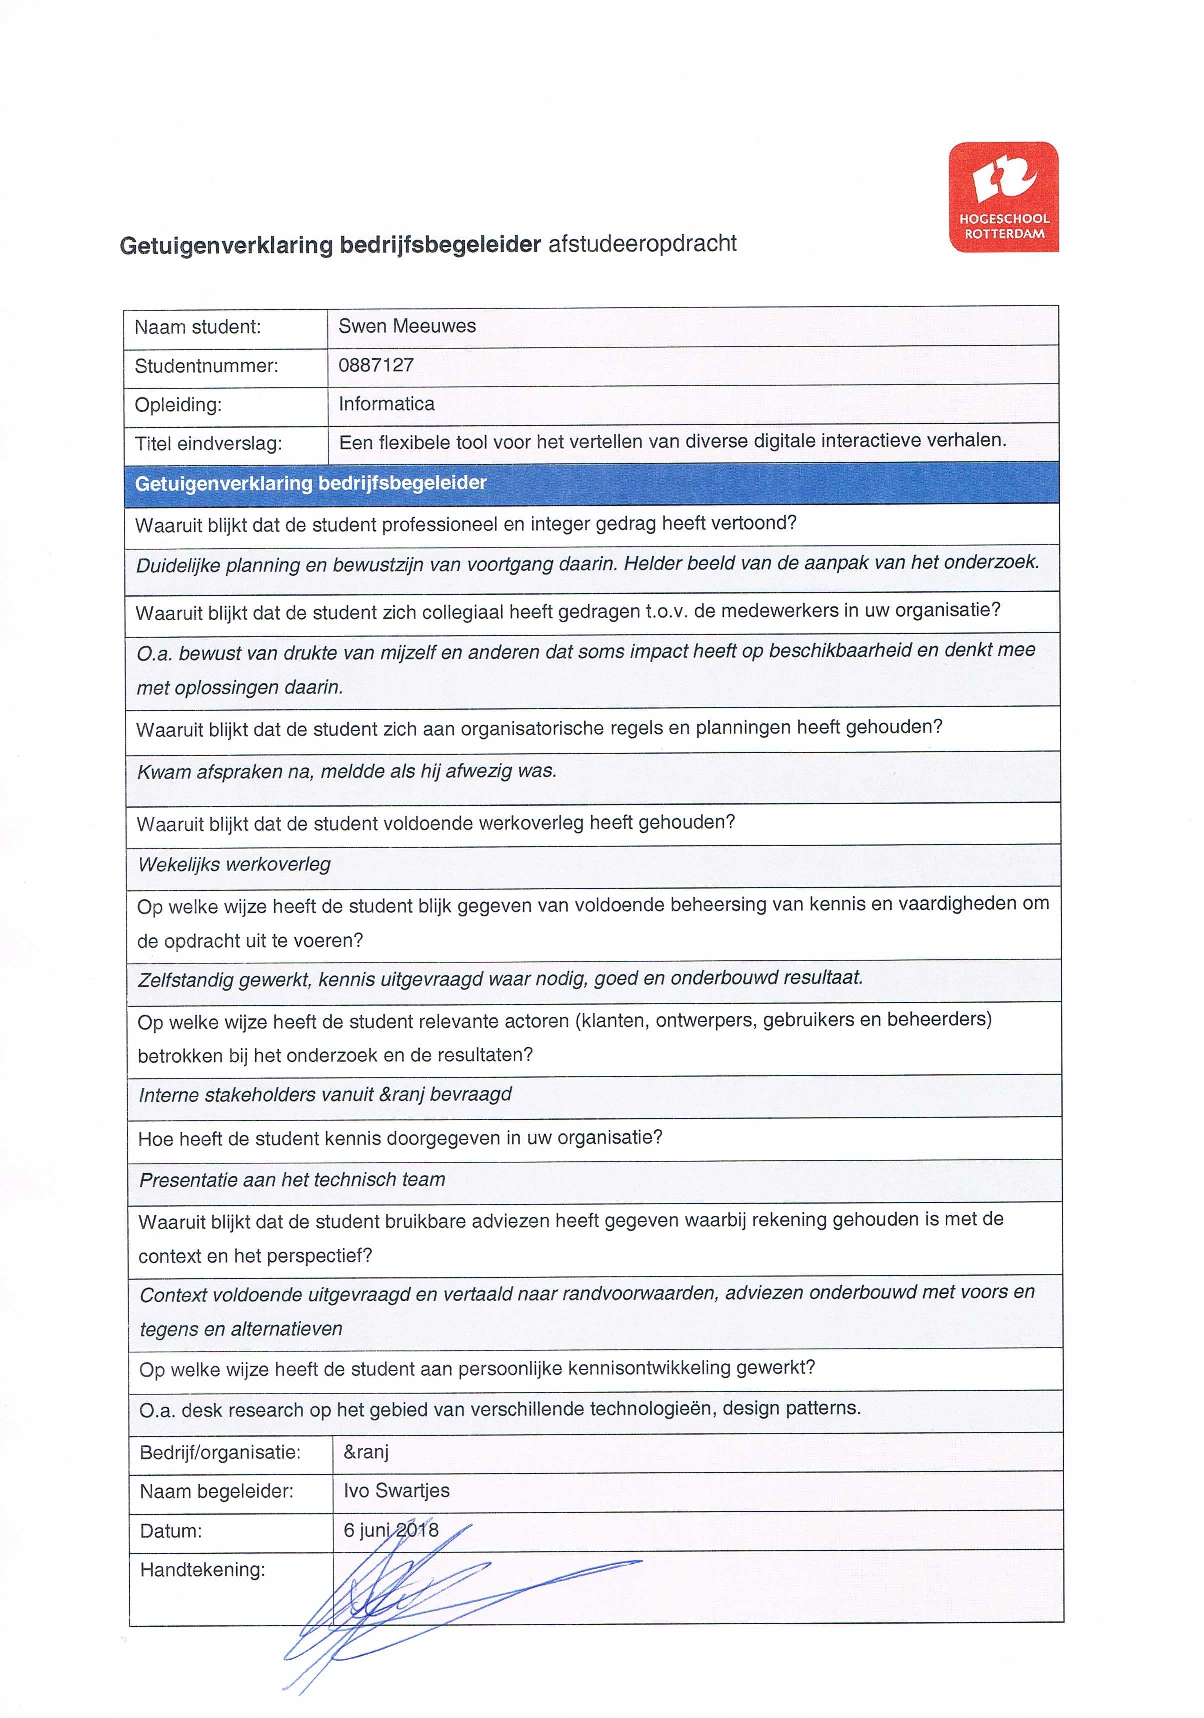
\includepdf[pages=-,scale=.75,offset=0mm -25mm,pagecommand=\chapter{Getuigenverklaringen}\label{app:getuigenverklaringen}]{assets/pdf/Getuigenverklaring_bedrijfsbegeleider.pdf}
    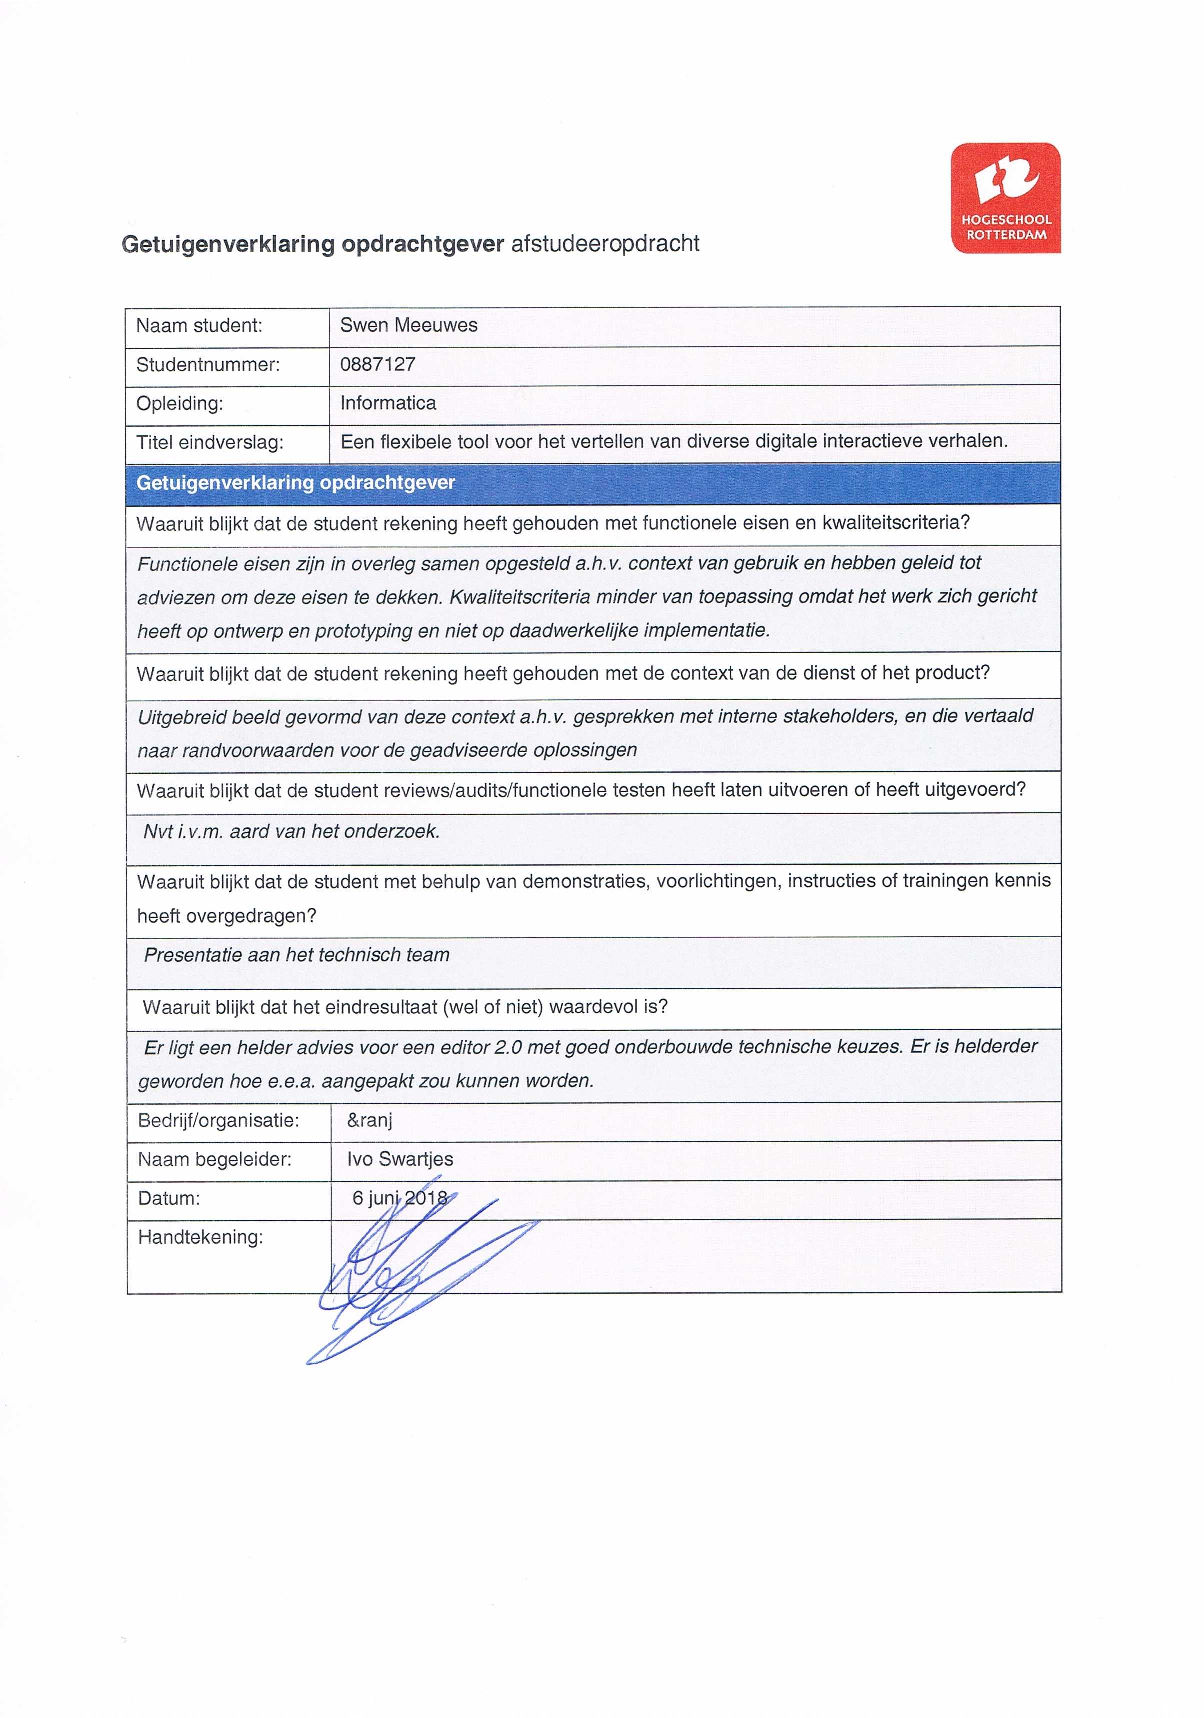
\includepdf[pages=-,scale=.75,pagecommand={}]{assets/pdf/Getuigenverklaring_opdrachtgever.pdf}
\end{appendices}

\end{document}
